\documentclass[11pt,a4paper,oneside]{book}
\usepackage[a4paper, portrait, margin=1.1in]{geometry}
% \documentclass[11pt,a4paper,twoside,openright]{book}
\usepackage{url}
\usepackage{makeidx}
\usepackage{listings}
\usepackage{graphicx}
\usepackage{fancyhdr}
\usepackage{fancyvrb}
\usepackage{parskip}
\usepackage{chngpage}
\usepackage{lmodern}
\usepackage{caption}
\usepackage{subcaption}
\usepackage[utf8]{inputenc}
% \usepackage{pdfpages}
% \usepackage[nottoc]{tocbibind}
\usepackage[toc,page,header]{appendix}
\usepackage[usenames,dvipsnames]{color}

\newcommand{\HRule}{\rule{\linewidth}{0.5mm}}
\renewcommand{\familydefault}{\sfdefault}


\definecolor{lightgray}{rgb}{.95,.95,.95}
\definecolor{darkgray}{rgb}{.4,.4,.4}
\definecolor{green}{rgb}{.2,.6,.0}
\definecolor{lightblue}{rgb}{.0,.5,.7}
\definecolor{purple}{rgb}{0.6, .1, 0.62}

\lstdefinelanguage{JavaScript}{
  keywords={typeof, new, true, false, catch, function, return, null, catch, switch, var, if, in, while, do, else, case, break, throw, for},
  keywordstyle=\color{blue}\bfseries,
  ndkeywords={exports, this, console},
  ndkeywordstyle=\color{lightblue}\bfseries,
  identifierstyle=\color{black},
  sensitive=false,
  comment=[l]{//},
  morecomment=[s]{/*}{*/},
  commentstyle=\color{green}\ttfamily,
  stringstyle=\color{purple}\ttfamily,
  morestring=[b]',
  morestring=[b]"
}

\lstdefinelanguage{Java}{
  keywords={typeof, new, true, false, catch, function, return, null, catch, switch, var, if, in, while, do, else, case, break, throw, String, Integer, int, Object, for, long, Runnable},
  keywordstyle=\color{blue}\bfseries,
  ndkeywords={import, this, class ,public, private, static, void, implements, extends},
  ndkeywordstyle=\color{lightblue}\bfseries,
  identifierstyle=\color{black},
  sensitive=false,
  comment=[l]{//},
  morecomment=[s]{/*}{*/},
  commentstyle=\color{green}\ttfamily,
  stringstyle=\color{purple}\ttfamily,
  morestring=[b]',
  morestring=[b]"
}

\lstdefinelanguage{KRE}{
  keywords={select, when, setting, with, http},
  keywordstyle=\color{blue}\bfseries,
  ndkeywords={rule},
  ndkeywordstyle=\color{lightblue}\bfseries,
  identifierstyle=\color{black},
  sensitive=false,
  morecomment=[s]{re\#}{\#},
  commentstyle=\color{green}\ttfamily,
  stringstyle=\color{purple}\ttfamily,
  morestring=[b]',
  morestring=[b]"
}

\lstdefinelanguage{OwnRule}{
  keywords={expression, event, condition, action, selector, symbol, instr, <, ==, >, >=, <=},
  keywordstyle=\color{blue}\bfseries,
  ndkeywords={on, if, do},
  ndkeywordstyle=\color{lightblue}\bfseries,
  identifierstyle=\color{black},
  sensitive=false,
  morecomment=[s]{re\#}{\#},
  commentstyle=\color{green}\ttfamily,
  stringstyle=\color{purple}\ttfamily,
  morestring=[b]',
  morestring=[b]"
}

% \lstdefinelanguage{JSON}{
%   identifierstyle=\color{black},
%   sensitive=false,
%   stringstyle=\color{purple}\ttfamily,
%   morestring=[b]',
%   morestring=[b]"
% }

% \definecolor{numb}{RGB}{150, 150, 150}
% \definecolor{delim}{RGB}{20,105,176}

% \lstdefinelanguage{JSON}{
%   identifierstyle=\color{black},
%   sensitive=false,
%   stringstyle=\color{purple}\ttfamily,
%   morestring=[b]',
%   morestring=[b]",
%     literate=
%      *{0}{{{\color{numb}0}}}{1}
%       {1}{{{\color{numb}1}}}{1}
%       {2}{{{\color{numb}2}}}{1}
%       {3}{{{\color{numb}3}}}{1}
%       {4}{{{\color{numb}4}}}{1}
%       {5}{{{\color{numb}5}}}{1}
%       {6}{{{\color{numb}6}}}{1}
%       {7}{{{\color{numb}7}}}{1}
%       {8}{{{\color{numb}8}}}{1}
%       {9}{{{\color{numb}9}}}{1}
%       % {\{}{{{\color{delim}{\{}}}}{1}
%       % {\}}{{{\color{delim}{\}}}}}{1}
%       % {[}{{{\color{delim}{[}}}}{1}
%       % {]}{{{\color{delim}{]}}}}{1}
% }

\lstdefinelanguage{RDF}{
  keywords={on, insert, if, do, delete, let, in},
  keywordstyle=\color{blue}\bfseries,
  % keywords=[2]{delta},
  % keywordstyle=[2]\color{green}\bfseries,
  ndkeywords={document, resource},
  ndkeywordstyle=\color{lightblue}\bfseries,
  identifierstyle=\color{black},
  sensitive=false,
  comment=[l]{//},
  morecomment=[s]{/*}{*/},
  commentstyle=\color{green}\ttfamily,
  stringstyle=\color{purple}\ttfamily,
  morestring=[b]',
  morestring=[b]"
}

\lstdefinelanguage{N3}{
  alsoletter=?,
  keywords={ ?x },
  keywordstyle=\color{blue}\bfseries,
  ndkeywords={exports, this},
  ndkeywordstyle=\color{lightblue}\bfseries,
  identifierstyle=\color{black},
  sensitive=false,
  comment=[l]{//},
  morecomment=[s]{/*}{*/},
  commentstyle=\color{green}\ttfamily,
  stringstyle=\color{purple}\ttfamily,
  morestring=[b]',
  morestring=[b]"
}

\lstdefinelanguage{XChange}{
  keywords={TRANSACTION, on, end, in, insert, from},
  keywordstyle=\color{blue}\bfseries,
  ndkeywords={xchange, var, resource},
  ndkeywordstyle=\color{lightblue}\bfseries,
  identifierstyle=\color{black},
  sensitive=false,
  comment=[l]{//},
  morecomment=[s]{/*}{*/},
  commentstyle=\color{green}\ttfamily,
  stringstyle=\color{purple}\ttfamily,
  morestring=[b]',
  morestring=[b]"
}

\lstset{
  language=JavaScript,
  % backgroundcolor=\color{lightgray},
  basicstyle=\footnotesize\ttfamily,
  extendedchars=true,
  frame=single,
  showstringspaces=false,
  showspaces=false,
  numbers=left,
  numberstyle=\tiny,
  numbersep=9pt,
  tabsize=2,
  breaklines=true,
  showtabs=false,
  captionpos=b,
  aboveskip=10pt,
  belowskip=10pt,
  xleftmargin=.3in
  % frameround=tttt,
  % boxpos=t
}


\makeatletter
\def\PY@reset{\let\PY@it=\relax \let\PY@bf=\relax%
    \let\PY@ul=\relax \let\PY@tc=\relax%
    \let\PY@bc=\relax \let\PY@ff=\relax}
\def\PY@tok#1{\csname PY@tok@#1\endcsname}
\def\PY@toks#1+{\ifx\relax#1\empty\else%
    \PY@tok{#1}\expandafter\PY@toks\fi}
\def\PY@do#1{\PY@bc{\PY@tc{\PY@ul{%
    \PY@it{\PY@bf{\PY@ff{#1}}}}}}}
\def\PY#1#2{\PY@reset\PY@toks#1+\relax+\PY@do{#2}}

\expandafter\def\csname PY@tok@gd\endcsname{\def\PY@tc##1{\textcolor[rgb]{0.63,0.00,0.00}{##1}}}
\expandafter\def\csname PY@tok@gu\endcsname{\let\PY@bf=\textbf\def\PY@tc##1{\textcolor[rgb]{0.50,0.00,0.50}{##1}}}
\expandafter\def\csname PY@tok@gt\endcsname{\def\PY@tc##1{\textcolor[rgb]{0.00,0.27,0.87}{##1}}}
\expandafter\def\csname PY@tok@gs\endcsname{\let\PY@bf=\textbf}
\expandafter\def\csname PY@tok@gr\endcsname{\def\PY@tc##1{\textcolor[rgb]{1.00,0.00,0.00}{##1}}}
\expandafter\def\csname PY@tok@cm\endcsname{\let\PY@it=\textit\def\PY@tc##1{\textcolor[rgb]{0.25,0.50,0.50}{##1}}}
\expandafter\def\csname PY@tok@vg\endcsname{\def\PY@tc##1{\textcolor[rgb]{0.10,0.09,0.49}{##1}}}
\expandafter\def\csname PY@tok@m\endcsname{\def\PY@tc##1{\textcolor[rgb]{0.40,0.40,0.40}{##1}}}
\expandafter\def\csname PY@tok@mh\endcsname{\def\PY@tc##1{\textcolor[rgb]{0.40,0.40,0.40}{##1}}}
\expandafter\def\csname PY@tok@go\endcsname{\def\PY@tc##1{\textcolor[rgb]{0.53,0.53,0.53}{##1}}}
\expandafter\def\csname PY@tok@ge\endcsname{\let\PY@it=\textit}
\expandafter\def\csname PY@tok@vc\endcsname{\def\PY@tc##1{\textcolor[rgb]{0.10,0.09,0.49}{##1}}}
\expandafter\def\csname PY@tok@il\endcsname{\def\PY@tc##1{\textcolor[rgb]{0.40,0.40,0.40}{##1}}}
\expandafter\def\csname PY@tok@cs\endcsname{\let\PY@it=\textit\def\PY@tc##1{\textcolor[rgb]{0.25,0.50,0.50}{##1}}}
\expandafter\def\csname PY@tok@cp\endcsname{\def\PY@tc##1{\textcolor[rgb]{0.74,0.48,0.00}{##1}}}
\expandafter\def\csname PY@tok@gi\endcsname{\def\PY@tc##1{\textcolor[rgb]{0.00,0.63,0.00}{##1}}}
\expandafter\def\csname PY@tok@gh\endcsname{\let\PY@bf=\textbf\def\PY@tc##1{\textcolor[rgb]{0.00,0.00,0.50}{##1}}}
\expandafter\def\csname PY@tok@ni\endcsname{\let\PY@bf=\textbf\def\PY@tc##1{\textcolor[rgb]{0.60,0.60,0.60}{##1}}}
\expandafter\def\csname PY@tok@nl\endcsname{\def\PY@tc##1{\textcolor[rgb]{0.63,0.63,0.00}{##1}}}
\expandafter\def\csname PY@tok@nn\endcsname{\let\PY@bf=\textbf\def\PY@tc##1{\textcolor[rgb]{0.00,0.00,1.00}{##1}}}
\expandafter\def\csname PY@tok@no\endcsname{\def\PY@tc##1{\textcolor[rgb]{0.53,0.00,0.00}{##1}}}
\expandafter\def\csname PY@tok@na\endcsname{\def\PY@tc##1{\textcolor[rgb]{0.49,0.56,0.16}{##1}}}
\expandafter\def\csname PY@tok@nb\endcsname{\def\PY@tc##1{\textcolor[rgb]{0.00,0.50,0.00}{##1}}}
\expandafter\def\csname PY@tok@nc\endcsname{\let\PY@bf=\textbf\def\PY@tc##1{\textcolor[rgb]{0.00,0.00,1.00}{##1}}}
\expandafter\def\csname PY@tok@nd\endcsname{\def\PY@tc##1{\textcolor[rgb]{0.67,0.13,1.00}{##1}}}
\expandafter\def\csname PY@tok@ne\endcsname{\let\PY@bf=\textbf\def\PY@tc##1{\textcolor[rgb]{0.82,0.25,0.23}{##1}}}
\expandafter\def\csname PY@tok@nf\endcsname{\def\PY@tc##1{\textcolor[rgb]{0.00,0.00,1.00}{##1}}}
\expandafter\def\csname PY@tok@si\endcsname{\let\PY@bf=\textbf\def\PY@tc##1{\textcolor[rgb]{0.73,0.40,0.53}{##1}}}
\expandafter\def\csname PY@tok@s2\endcsname{\def\PY@tc##1{\textcolor[rgb]{0.73,0.13,0.13}{##1}}}
\expandafter\def\csname PY@tok@vi\endcsname{\def\PY@tc##1{\textcolor[rgb]{0.10,0.09,0.49}{##1}}}
\expandafter\def\csname PY@tok@nt\endcsname{\let\PY@bf=\textbf\def\PY@tc##1{\textcolor[rgb]{0.00,0.50,0.00}{##1}}}
\expandafter\def\csname PY@tok@nv\endcsname{\def\PY@tc##1{\textcolor[rgb]{0.10,0.09,0.49}{##1}}}
\expandafter\def\csname PY@tok@s1\endcsname{\def\PY@tc##1{\textcolor[rgb]{0.73,0.13,0.13}{##1}}}
\expandafter\def\csname PY@tok@sh\endcsname{\def\PY@tc##1{\textcolor[rgb]{0.73,0.13,0.13}{##1}}}
\expandafter\def\csname PY@tok@sc\endcsname{\def\PY@tc##1{\textcolor[rgb]{0.73,0.13,0.13}{##1}}}
\expandafter\def\csname PY@tok@sx\endcsname{\def\PY@tc##1{\textcolor[rgb]{0.00,0.50,0.00}{##1}}}
\expandafter\def\csname PY@tok@bp\endcsname{\def\PY@tc##1{\textcolor[rgb]{0.00,0.50,0.00}{##1}}}
\expandafter\def\csname PY@tok@c1\endcsname{\let\PY@it=\textit\def\PY@tc##1{\textcolor[rgb]{0.25,0.50,0.50}{##1}}}
\expandafter\def\csname PY@tok@kc\endcsname{\let\PY@bf=\textbf\def\PY@tc##1{\textcolor[rgb]{0.00,0.50,0.00}{##1}}}
\expandafter\def\csname PY@tok@c\endcsname{\let\PY@it=\textit\def\PY@tc##1{\textcolor[rgb]{0.25,0.50,0.50}{##1}}}
\expandafter\def\csname PY@tok@mf\endcsname{\def\PY@tc##1{\textcolor[rgb]{0.40,0.40,0.40}{##1}}}
%\expandafter\def\csname PY@tok@err\endcsname{\def\PY@bc##1{\setlength{\fboxsep}{0pt}\fcolorbox[rgb]{1.00,0.00,0.00}{1,1,1}{\strut ##1}}}
\expandafter\def\csname PY@tok@kd\endcsname{\let\PY@bf=\textbf\def\PY@tc##1{\textcolor[rgb]{0.00,0.50,0.00}{##1}}}
\expandafter\def\csname PY@tok@ss\endcsname{\def\PY@tc##1{\textcolor[rgb]{0.10,0.09,0.49}{##1}}}
\expandafter\def\csname PY@tok@sr\endcsname{\def\PY@tc##1{\textcolor[rgb]{0.73,0.40,0.53}{##1}}}
\expandafter\def\csname PY@tok@mo\endcsname{\def\PY@tc##1{\textcolor[rgb]{0.40,0.40,0.40}{##1}}}
\expandafter\def\csname PY@tok@kn\endcsname{\let\PY@bf=\textbf\def\PY@tc##1{\textcolor[rgb]{0.00,0.50,0.00}{##1}}}
\expandafter\def\csname PY@tok@mi\endcsname{\def\PY@tc##1{\textcolor[rgb]{0.40,0.40,0.40}{##1}}}
\expandafter\def\csname PY@tok@gp\endcsname{\let\PY@bf=\textbf\def\PY@tc##1{\textcolor[rgb]{0.00,0.00,0.50}{##1}}}
\expandafter\def\csname PY@tok@o\endcsname{\def\PY@tc##1{\textcolor[rgb]{0.40,0.40,0.40}{##1}}}
\expandafter\def\csname PY@tok@kr\endcsname{\let\PY@bf=\textbf\def\PY@tc##1{\textcolor[rgb]{0.00,0.50,0.00}{##1}}}
\expandafter\def\csname PY@tok@s\endcsname{\def\PY@tc##1{\textcolor[rgb]{0.73,0.13,0.13}{##1}}}
\expandafter\def\csname PY@tok@kp\endcsname{\def\PY@tc##1{\textcolor[rgb]{0.00,0.50,0.00}{##1}}}
\expandafter\def\csname PY@tok@w\endcsname{\def\PY@tc##1{\textcolor[rgb]{0.73,0.73,0.73}{##1}}}
\expandafter\def\csname PY@tok@kt\endcsname{\def\PY@tc##1{\textcolor[rgb]{0.69,0.00,0.25}{##1}}}
\expandafter\def\csname PY@tok@ow\endcsname{\let\PY@bf=\textbf\def\PY@tc##1{\textcolor[rgb]{0.67,0.13,1.00}{##1}}}
\expandafter\def\csname PY@tok@sb\endcsname{\def\PY@tc##1{\textcolor[rgb]{0.73,0.13,0.13}{##1}}}
\expandafter\def\csname PY@tok@k\endcsname{\let\PY@bf=\textbf\def\PY@tc##1{\textcolor[rgb]{0.00,0.50,0.00}{##1}}}
\expandafter\def\csname PY@tok@se\endcsname{\let\PY@bf=\textbf\def\PY@tc##1{\textcolor[rgb]{0.73,0.40,0.13}{##1}}}
\expandafter\def\csname PY@tok@sd\endcsname{\let\PY@it=\textit\def\PY@tc##1{\textcolor[rgb]{0.73,0.13,0.13}{##1}}}
%\expandafter\def\csname PY@tok@err\endcsname{}

\def\PYZbs{\char`\\}
\def\PYZus{\char`\_}
\def\PYZob{\char`\{}
\def\PYZcb{\char`\}}
\def\PYZca{\char`\^}
\def\PYZam{\char`\&}
\def\PYZlt{\char`\<}
\def\PYZgt{\char`\>}
\def\PYZsh{\char`\#}
\def\PYZpc{\char`\%}
\def\PYZdl{\char`\$}
\def\PYZhy{\char`\-}
\def\PYZsq{\char`\'}
\def\PYZdq{\char`\"}
\def\PYZti{\char`\~}
% for compatibility with earlier versions
\def\PYZat{@}
\def\PYZlb{[}
\def\PYZrb{]}
\makeatother

% How deep numbering is applied to titles
% \setcounter{secnumdepth}{3}
\setcounter{tocdepth}{1}

% Prepare the word index
\makeindex

% Prepare header and footer
\pagestyle{fancy}
\fancyhf{}
\rhead{\footnotesize\leftmark}
\lfoot{Towards the Reactive Web}
\rfoot{\thepage}
\renewcommand{\headrulewidth}{0.3pt}
\renewcommand{\footrulewidth}{0.3pt}

% Apply page style also to chapter's first page
\makeatletter
\renewcommand\chapter{\if@openright\cleardoublepage\else\clearpage\fi
  \thispagestyle{fancy}%
  \global\@topnum\z@
  \@afterindentfalse
  \secdef\@chapter\@schapter}
\makeatother

\setlength{\parindent}{15pt}
% \setlength{\parskip}{.5\baselineskip}%

\begin{document}

\frontmatter
	\begin{titlepage}
\begin{center}

% \title{\huge \textbf{Towards The Reactive Web}\vspace*{15 mm}}
% %\subtitle{Master Thesis Report}
% \date{\today}
% %\date{}
% %\author{Dominic Bosch \\ Departement Mathematics and Computer Science \\ University of Basel}
% \author{\fontsize{11}{9}\selectfont
% Master Thesis\\
% \vspace*{10 mm}\\
% Dominic Bosch\\
% Departement Mathematics and Computer Science\\
% University of Basel
% }
% \maketitle

\vspace*{4cm}
\HRule \\[0.4cm]
{ \huge \bfseries Towards Reactive Information Systems \\ and their Services \\[0.4cm] }
% { \huge \bfseries Towards The Reactive Web \\[0.4cm] }
\HRule \\[1.5cm]

% \textsc{\Large Departement Mathematics and Computer Science}\\[0.5cm]

\vspace*{.5cm}
\textit{\textsc{\LARGE Master Thesis}}\\
\vspace*{2.5cm}

% Author and supervisor
\begin{minipage}{0.4\textwidth}
\begin{flushleft} \large
\emph{Author:}\\
Dominic \textsc{Bosch}
\end{flushleft}
\end{minipage}
\begin{minipage}{0.4\textwidth}
\begin{flushright} \large
\emph{Supervisors:} \\
Prof. Dr.~Helmar \textsc{Burkhart}\\
Dr.~Martin \textsc{Guggisberg}
\end{flushright}
\end{minipage}

\vfill

% Bottom of the page
{\large \today} \\[1.5cm]
% {\large May 15, 2014} \\[1.5cm]



% \textsc{\LARGE University of Basel}\\

\includegraphics[width=0.15\textwidth]{figures/unilogoschwarz}%~\\[1cm]
\end{center}
\end{titlepage}

	% \chapter*{Acknowledgment}
I would like to express my deep gratitude to my master thesis advisor, Prof. Dr. Helmar Burkhart, for his patience and constant encouragement to keep going further.
I also want to thank Dr. Martin Guggisberg for his very helpful advices and hints to existing technologies.
Besides my advisors, I would like to thank the members of the research group: Danilo Guerrera,
Antonio Maffia, Alexander Gr\"oflin and Robert Frank for their help, many interesting discussions and inputs.

I would like to thank my parents Silvia and Peter Bosch for their love, patience and financial support on my journey.
Special thanks go to my sister Svenja, her husband Andreas and their seven months old son Nico, who all kept me going with their joyfulness and irresistble smiles.
Finally I would like to thank my partner Kathrina Hagnauer for her patience and endless love.
	\tableofcontents
	\listoffigures
	% FIXME CHECK WHETHER TABLES OR LISTINGS ARE IN THE DOCUMENT
	% \listoftables
	% \lstlistoflistings

\mainmatter
	
\chapter{Introduction}

The web is an ever growing entity, in all aspects that it covers.
It surrounds a growing number of human beings in their daily life and starts to overwhelm them with an information flood.
One example of this information flood is the one hundred hours of video material that is uploaded to youtube\cite{wwwYoutube} every single minute.
An increasing number of bigger computing centers, but also ever smaller devices provide more data and functionality, both in quantity and complexity.
Also, a growing fraction of these devices have access to the web, which means they are potential data and functionality resources.
A white paper\cite{citeulike:12243016} estimates that 200 million devices were connected to the internet in the year 2000.
They also estimate that this number raised up to approximately 10 billion connected devices in 2013.
Further more, they expect this number to grow up to 50 billion connected devices by the year 2020.
This alone shows how strong growth of potentially data and functionalty delivering devices is growing currently and in the near future.
Other recent research\cite{conf/icws/HuangFT12}\cite{wwwProgrammableWebResearch} has shown that the number of accessible Web APIs follows power law distribution and thus provides an ever growing source of data and functionality.
The ever smaller devices that make up the "Internet of Things"\cite{Weber2010} today, are also capable of spreading the ubiquitous access to the web, e.g. through mobile devices.
 % and their push notifications, users get flooded with informations and, in turn, also produce increasingly more information.

The human being requires tools to get the right information in the right situation at the right place and also to automate tasks
user-centric reactions to allow a personalization of the information flood
Governing the web's information flood is getting more difficult and even fairly impossible for human beings with the tools given.


It becomes important to the individual to be able to filter out personally important bits and pieces.
Basic filters are often available but they do not allow smart filtering in any way.
Also, apart from smart filtering of information, people should have the possibility to aggregate important information in their desired place and in a way it's most useful for themselves.
Such an aggregation implies access to services that consume data and produce an output, be it a data answer or storage.
This means the user should get access to data and functionality services in a way that she can combine the possibilities in a suitable way to generated the most valuable output for her.
Even if the web service access gets simpler these days, the average user is not able to weild them.
The challenge to provide users with ways to handle these already simpler accessible services, called Web API's has received a notable amount of attention over the last few years.

% % TODO Reactivity!! allgemein
% \index{Reactivity}

% % TODO Programmability of the Web
% \index{Programmability}
%  -> in general, both should go into related work?

% TODO Information Space\cite{conf/trec/Newby96}
% Information space is a set of concepts and relations among them held by an information system.
% Information space is produced by a set of known procedures, and is changed through intentional
% manipulation of its content.

It is a promising research field that leads towards reactivity in the web through programmability.
Currently somebody that want's to program the web, requires deep knowledge of the required services and their functionality.
There are a few possibilities in the web that go towards easing the programmability of the web, but they are either complicated to weild themselves or mere data copy or mashup tasks.
Our research in this thesis is about easing the programmability of the web and therefore to achieve the reactive web. 

	
\chapter{Related Work}

In this chapter we will give a brief overview over different services offered in the Web, to point out what services in the Web all can be.
We then introduce the Event-Condition-Action (\textrm{ECA}) paradigm, an event-driven approach to impose reactivity.
And finally we point out existing rule languages and engines that exploit the \textrm{ECA} paradigm.



\section{Services in the Web}
The term service in the context of the Web is ambiguous and there have been a lot of different approaches to offer services within the Web.
\index{Web Service}
\index{Services}
\index{World Wide Web}
For example the term \textrm{Web Services} often refers to interfaces that are used in the \textrm{World Wide Web} for communication between applications.
We will point out some main research areas on service-orientation within the Web.

Remote execution of programs on other computers has always been a strong research area. And with the coinage of the term \textrm{World Wide Web}~\cite{DBLP:journals/en/Berners-LeeCGP92}, there were also trends towards services offered through the Web; computers waiting in the Web for a request in order to execute some application logic and return an answer.
\index{SOA}
The encapsulation of functionality into services~\cite{peltz2003web} in order to offer them to other applications is called service-oriented architecture (\textrm{SOA})~\cite{perrey2003service}.
Adopting \textrm{SOA} internally to an application means splitting the application into smaller pieces, which then communiacte via these services among each other.
This does not only provide robustness, it also allows the reuse of functionality through services.
Moreover these services can be offered to other applications and also to the Web, thus allowing others to access certain functionalty or even the whole application.
All nodes in the Web are stand-alone entities, which offer services of some sort, be it a webpage, data, instant measurements or functionality.
This makes the Web itself a service-oriented architecture and all these services are naturally services in the Web.
It is for its advantages that \textrm{SOA} has received a great deal of attention and has been widely adopted, mostly throughout the Web.
This lead to an increasing number of Web accessible services and their compositions, the so called \textrm{Mashups}.
An empirical study~\cite{conf/icws/HuangFT12} on a directory, which they call the \textit{"[...] most active Web APIs and mashups collection"}, and data taken from this resource (depicted in Figure \ref{fig:NumOfAPIs}) seem to underline a growing popularity, at least in terms of publishing services through this directory.

\begin{figure}[!ht]
  \centering
  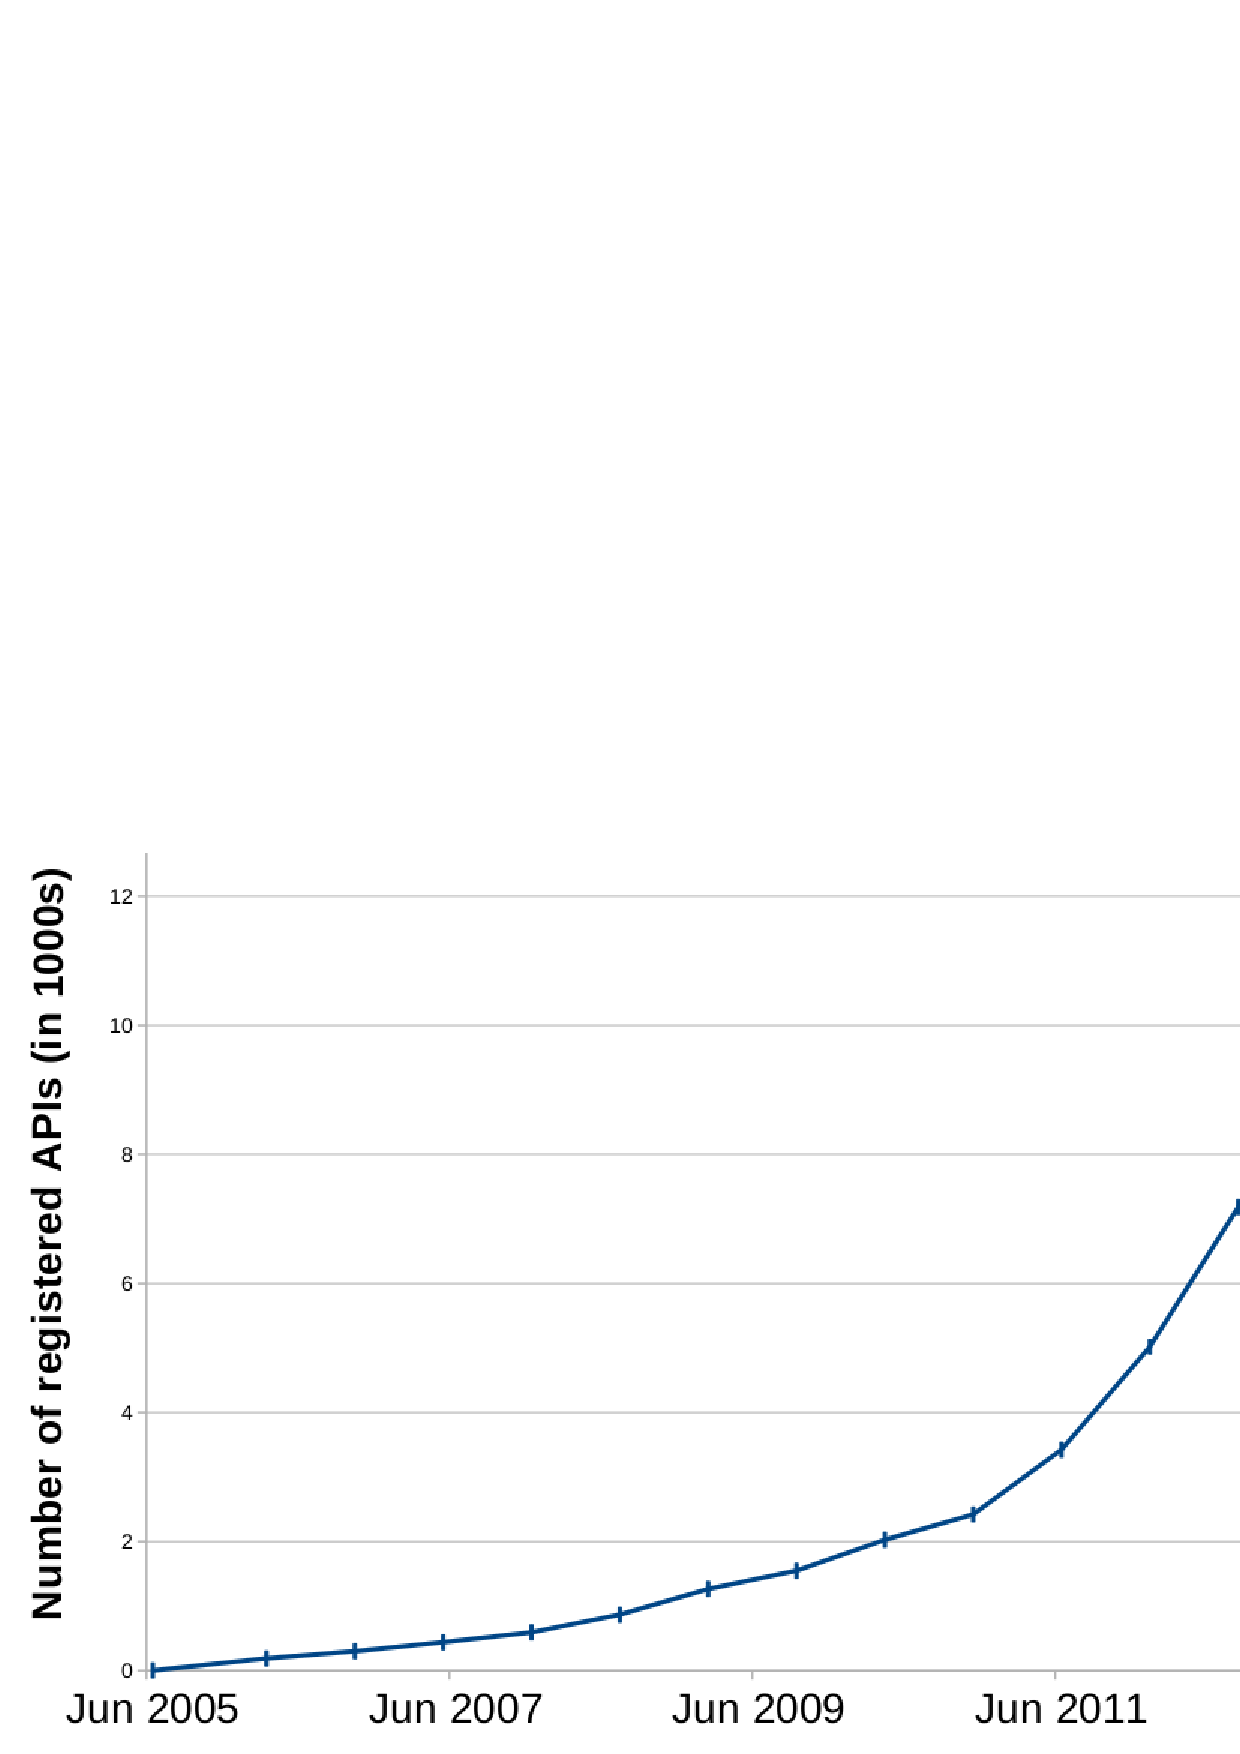
\includegraphics[width=0.55\textwidth]{figures/NumOfAPIs}
  \caption{Number of registered APIs in the ProgrammableWeb directory by date}
  \label{fig:NumOfAPIs}
\end{figure}


\subsection{Requesting Services in the Web}
\index{RPC}
An early adoption of the service concept to computers were the Remote Procedure Calls (\textrm{RPC})~\cite{Birrell:1984:IRP:2080.357392}.
Through \textrm{RPC} a piece of code can be executed on a different machine, than the one which is calling the procedure.
It is basically achieved via inter-process communication and doesn't necessarily require the Web.
Even more since when \textrm{RPC} was invented, the \textrm{World Wide Web} wasn't even postulated by Tim Berners-Lee. 
\textrm{RPC} also found its use in grid computing~\cite{seymour2002overview} and through this, opened doors into the field of distributed computation.
The \textrm{RPC} paradigm isn't bound to certain technologies and thus, has been implemented in a lot of differrent programming languages.
These implementations were tightly bound to the respective language that was used, which resulted largely in incomptaiblity among them.
\index{XML}
\index{XML-RPC}
It became necessary to enhance \textrm{RPC}'s in order to get cross platform compatibility.
By abstracting \textrm{RPC} functionality with the Extensible Markup Language (\textrm{XML})~\cite{bray1998extensible}, compatibility between services that used different technologies was easier to achieve.

\index{SOAP}
\index{WSDL}
Since \textrm{XML-RPC} was held relatively simple but received a lot of attention, it was further enhanced.
Together with additional proposedy functionality, XML-RPC heavily influenced Simple Object Access Protocol (\textrm{SOAP})~\cite{box2000simple}.
\textrm{SOAP} is accompanied by the Web Service Description Language (\textrm{WSDL})~\cite{christensen2001web} which is used to describe the interfaces to SOAP services.
Through \textrm{SOAP} and \textrm{WSDL} a client for the service can issue a request for the \textrm{WSDL} information of the service and retrieves all interface specifications he requires in order to issue a call to the actual service.
The service specifications are then incorporated into the existing application as if it is a local function call.
\textrm{SOAP} has found its applicability in business applications~\cite{journals/itpro/BarrosD06} and was enhanced with a lot of industrial standards, also called the "WS-*" specifications, e.g. WS-Addressing, WS-Policy or WS-Security.

\index{CORBA}
Another initiative that aimed for eased communication between different platform is the Common Object Request Broker Architecture (\textrm{CORBA})~\cite{dec1991common}.
As the name already suggest it is an object-oriented approach and it allows the exchange of whole objects.
\index{ORB}
\textrm{CORBA} relies on its communication layer, the Object Request Broker (\textrm{ORB}), which forms the basis of its architecture.
The platform-specific \textrm{ORB}'s provide the communication abstraction, which free the application from platform dependencies.
\index{IDL}
Similar to \textrm{SOAP}'s \textrm{WSDL}, \textrm{CORBA} has its Interface Definition Languange (\textrm{IDL}) to provide information about the objects to be offered and accessed.
An object is instantiated by an application and the interface to this instance is offered through the \textrm{ORB}.
Another application attached to the \textrm{ORB} can then access all public variables, data structures and functions of this object.
This means not only remote access to variables and data structures, but also remote function invocation.
\textrm{CORBA} requires the implementation of object-oriented mechanisms in programming languages which aren't object-oriented.
This can be technically difficult and become an eventually tedious task.
\textrm{CORBA} allows communication between applications written in different programming languages and which are running on the same physical computer, as well as the communication between different computers in the same network.
With the Internet Inter-\textrm{ORB} Protocol (\textrm{IIOP}) it is also possible to connect \textrm{ORB}'s over the Web.
Through this, the offered objects can become services in the Web, but they are shielded by the \textrm{ORB}.

\subsection{Services in the Web become Web Resources}
\index{REST}
All the afore mentioned approaches require a specific protocol and are therefore incompatible with each other.
For this reason and its simplicity, an architectural style has gained popularity which frees application from this constraint: Representational State Transfer (\textrm{REST})~\cite{fielding2000architectural}.
\textrm{REST} concentrates on the roles of components and on constraints upon interactions between them.
An important architectural constraint is that all communication is stateless, which means for a client-server communication, no state is stored on the server.
Therefore all informations required for a single interaction need to be provided within one request.
This allows for the definition of simple and well-defined interfaces, since responses are not bound to a certain session state. 
\index{REST}
Services within the Web that adhere to the \textrm{REST} architecture are called \textrm{RESTful} Web services.
\index{URI}
\index{Web Resources}
\textrm{RESTful} Web services provide access to their data and functionality through grouped \textrm{Web Resources}, which can be identified vie Uniform Resource Identifiers (\textrm{URI}).
Simple access to services in the Web without communication overhead and required negotiation before using it, increased \textrm{REST}'s popularity and spread it into more application fields.
There is for example the upcoming concept of the \textrm{Web of Things}~\cite{Guinard2011WoT}, which aims to incorporate smart things (e.g. tagged things, sensor measurements, device controllers, etc.) into the Web through \textrm{REST} interfaces.
\textrm{REST} brings advantages into the context of smart things connected to the Web, because incompatible standards and protocols were used by different manufacturers of such things.


\subsection{Composing Services in the Web}
% \section{Weakening the Relevance of the Client-Server Model}
% \textit{Dropping the Client-Server Model}\\
% \textit{The Interweavement of Client and Server}\\
Webpages emerged into dynamic sites on the web through the upcoming of scripting languages to control the browser and the webpage itself.
With all their infrastructure in the background on the server they became literally applications.
\index{Web Application}
These Web applications (\textrm{Web Apps}) went even more responsive with the advent of asynchronous calls from the browser to the server, which allows to load data into the current webpage while the user is interacting with it.
\index{API}
\index{Web API}
Those asynchronous calls are requests to services, which act as the application programming interface \textrm{API} to the \textrm{Web App} (\textrm{Web APIs}) which sits on the server.
As a side-note, the term \textrm{Web API} not only comprises server-side interfaces but also client-sided ones (e.g. the browser), after all they are also interfaces to the Web.
For server-side \textrm{Web APIs} this means that these services can be accessed from other entities in the Web than just browsers, which eases application to application communication.
Basically a \textrm{Web App} can be controlled without the user interface, which is often delivered by the provider of the application.
Imagine not going to the Google webpage anymore to make a search and crawling through the results, but you have your own application doing it for you and processing the results instantly.
There is a trend of \textrm{Web App} providers to publish their \textrm{Web API} in order to grant easy access to it.
This lead to an increase of the number of \textrm{Web App Mashups} in the past few years.

\index{Mashup}
\textrm{Mashups} combine data and functionality of more than one service in the Web in a new site.
Simple services from different sources can be combined into more powerful ones, which can in turn again be composed and so on.
These service compositions assemble data and services in a novel way which provides a new perspective.
Ever since services were accessible in a more or less convenient way, \textrm{Mashups} have been developped as well.
On of the first Web service \textrm{Mashups}~\cite{wwwHosuingMaps}, was invented in the same year after Google Maps came up in 2005.
It was a webpage that displayed CraigsList's rental houses on a Google Map.
At that time no \textrm{Web API} was available that provided easy access to these two services, but there was an advantage to be seen from everybody being able to create a \textrm{Mashup} through publicly available services.
Such \textrm{Mashups} are often a read-only fixed wiring of different services that provide a new view on specific data.
Some recent \textrm{Mashup} examples, taken from the \textrm{ProgrammableWeb}~\cite{wwwProgrammableWeb} collection, are:

\begin{itemize}
  \item \textrm{Wifi and Plugs}: MapBox, Google Docs and Import.io API's used to display where Wi-Fi and plugs are available in London.
  \item \textrm{MapLight}: GovTrack.us and OpenSecrets API's used to combine political results with financial contributions to show how capital contributions to influence politics affect voting.
  \item \textrm{Shared Count}: Facebook, LinkedIn, Pinterest and Twitter API's used to display informations about how well spread a URL is on social media sites.
\end{itemize}

But also a number of studies ~\cite{10.1007/978-3-642-22233-7_11}\cite{4278815}\cite{Rizzotti:2010:UST:1772690.1772861}\cite{Stolee20131289} made efforts towards personalized \textrm{Mashups}, where users are capable of choosing what and how to link in order to enhance Web resources according to their needs.
These flexible \textrm{Mashup} applications often provide methods to access user-specific functionality within remote \textrm{Web Apps}, which makes them even more user-centered and customizable.


\subsection{Subscribing to Services in the Web}
There is another type of service in the Web which is quite the opposite to the afore mentioned approches in terms of the data flow.
\index{Webhooks}
\textrm{Webhooks} are a method that enables the asynchronous delivery of data whenever it gets available, compared to the need of actively requesting a service to deliver it.
They are unifrom resource identifiers (\textrm{URI}), which point to a service in the Web, which accepts the data delivered to it.
% ~\cite{Eugster:2003:MFP:857076.857078}
Within the publish/subscribe pardigm, such asynchronous delivery of data is referred to as events, since that's what the appearance of new data is.
\textrm{Webhooks} are callbacks that can be placed by a \textrm{Web App} provider or a user at a remote location, informing the data prolifering site about their interest in the data.
Both parties are services in the Web, since the \textrm{Webhook} providers accept the data delivered to their \textrm{URI} and the \textrm{Webhook} receipients offer to send the data.


\subsection{Towards Simple Access and Communication}
\index{JSON}
With JavaScript's success as browser scripting language and recently also as server-side programming language, JavaScript Object Notification (\textrm{JSON}) as an alternative to \textrm{XML} has become popular for data representation throughout the Web.
It is also because of its human-readable format and often simple parsing into data structures of existing programming languages.
There is a notable trend towards \textrm{RESTful} services in the Web that offer \textrm{JSON} communication.
\index{Web Programmability}
They benefit from simple but powerful interfaces and easy to debug human-readable communication, which eases integration into other applications, along with the reduced communication volume.
Together with client- and server-side \textrm{Web APIs} the Web becomes ever more programmable.



\section{Reactivity through Event-Condition-Action Rules}
\index{ECA}
In this chapter we have so far shown research in different areas that lead towards a programmable Web.
As a result of this research, it is getting easier to compose and orchestrate services in the Web, but reactivity needs to be programmed specifically by experts with the current state of services in the Web.
Several studies~\cite{2007_AlferesR3}\cite{2005-Bry_etal-XChange.pdf}\cite{10.1007-11896548_63}\cite{papamarkos2004rdftl}\cite{2012-Paschke_etal-ReactionRuleML.pdf} have been made on reactivity.
These studies suggest Event-Conditon-Action (\textrm{ECA}) rules as a convenient way to impose reactivity to a system.
\index{EDA}
As the name already suggests it bases on an event-driven architecture (\textrm{EDA}) and \textrm{ECA} rules consist of three parts:
\begin{itemize}
  \item Event: An event identifier, that enables detection of a triggered event
  \item Condition: Either Web queries or expressions to determine whether a rule should trigger the action
  \item Action: A set of instructions that complete the reactive behaviour
\end{itemize}

As a result of the above mentioned research, several different rule languages have been developped for different domains.
We will give a brief overview over the research which is closely related to our research domain, reactivity in the Web.


\subsection{Rule Engines \& Rule Languages}
\index{Rule Engine}
\index{Rule Language}
During our research we studied the different rule engines with respect to a certain use case, in order to determine their applicability for our studies.
The use case's ECA rule is:
\begin{itemize}
  \item Event: Receipt of an Email
  \item Condition: Check for a certain sender
  \item Action: Store it remotely via a Web API
\end{itemize}
The example event expressed in JSON can be found in Appendix \ref{lst:JSONEvent}.


Definition of events\cite{Adaikkalavan2007}


\begin{table}[ht]
  \centering
  \begin{tabular}{ | *{4}{l|} }
    \hline
    \textbf{Language} & \textbf{Event Type} & \textbf{Architecture} & \textbf{Actions} \\ \hline
    \textbf{RDFTL} & RDF Repositories & Distributed & (Local) RDF Repository \\ \hline
    \textbf{JSON Rules} & DOM Events & Centralized & Browser \\ \hline
    \textbf{XChange} & Web Resources & Disitributed & Local Web Resource \\ \hline
    \textbf{RuleML} & Web Resources & Disitributed & Local Web Resource \\ \hline
    \textbf{KRL} & Web Resources & Centralized & Local \& Remote Web Resource \\ \hline
  \end{tabular}
  \caption{Existing Rule Languages}
  \label{tab:rulelanguages}
\end{table}


% \begin{table}[ht]
%   \centering
%   \begin{tabular}{ | l | c | r | }
%     \hline
%     \textbf{Engine} & \textbf{Event Type} & \textbf{JSON Rules} \\ \hline
%     \textbf{JSON Rules} & DOM Events & 9 \\ \hline
%     \textbf{XChange} & Web Resources & 9 \\ \hline
%     \textbf{RuleML} & Web Resources & 9 \\ \hline
%   \end{tabular}
%   \caption{Existing Rule Engines}
%   \label{tab:ruleengines}
% \end{table}

Xchange geavily influenced our work

We defined an email event which the rule languages need to be able to process.
The JSON representation of the given email event as depicted in the appendix. %is shown in Listing~\ref{lstemail}.

% FIXME Leave out what was not inspiring!

\index{RDFTL}
An early ECA Rule Language for XML repositories
\textrm{RDFTL}~\cite{papamarkos2004rdftl} was postulated in 2003 and was picked up by many researches afterwards. It was designed to react on insert and delete events within RDF repositories and as an action change XML documents.
RDF desirable but who THE FUCK uses it

Now apart from implementing a rules engine, we would also need to add an XML document event manager which interpretes and pushes events into the XML file \emph{inbound\_queue.xml}. Then again this instance would interprete the ouptuts of the ECA engine, which would theoretically manifest in other XML documents, and produce meaningful actions on remote hosts. This wouldn't be an architecture which has its focus on the solution of our use case and, as a result, add complexity and create an unnecessary overhead.

\index{XChange}\index{Xcerpt}
% Web-specific capabilities, such as propagation of changes on the Web (change) and event-based communication between Web sites (exchange).
% peer-to-peer communication model
% push/pull strategy
% robustness
% ditrbuted systems
% hypotetical data
% since the web is far from having a unique architecture. meaning xchange would need to sit in each site for event comm aight?
% depends on remote locations understanding XChange
% XChange has nice event composition properties
% Xchange only consists of events no actions (actions are taken by remote systems through events received%)

The rule language XChange~\cite{2005-Patranjan-TLE.pdf} was the outcome of the REWERSE (~\cite{wwwRewerse}, Reasoning on the Web with Rules and Semantics) project, which was funded by the EU and Switzerland. Their work influenced a number of future research. The language was designed to add reactive behaviour to a "static" Web which is represented through XML resources. Thus we have action logics to alter such resources through insertions and deletions. Since we aim to utilize Web API's for our rule language we need a more generic approach which adds flexibility in term of the API provided. But the thorough research done with the language XChange holds valuable concepts, especially in terms of temporal evet composition. This could be a rule according to our use case:


But XChange is designed to access other resources in an action and thus provides powerful tools:

\index{JSON Rules}
In 2008 \emph{JSON Rules}~\cite{2008-Giurca_Pascalau-JSON_Rules.pdf} was introduced as a language to easily react on specific DOM tree compositions.
The usage of JavaScript allowed them to provide simple functions which could be called directly by the actions, thus abstracting functionality from the language.
This key concept found influence into our language as it allows different layers of abstractions.
Through this it is possible to provide generic functions for expert user as well as very limited functions with only few possibilities for parameterization to be used by unexperienced persons.
A drawback of this language is its binding to DOM tree events, where we would want to react on any events happening in the world.
Also the temporal composition to complex events is not a subject of their work and needs further attention.


\index{KRL}
A recent open-source development is the Kinetic Rules Engine together with the Kinetics Rule Language~~\cite{bookTheLiveWeb}.
It is built for the purpose of adding reactivity to the cloud.
The language is based on declarative syntax, enriched with imparative elements.
But it is a tedious task to get into a whole new language and their caveats.
\emph{authorization?}
% The KRE suits the demand for a certain coupling between the users browser and the remote rules engine to provide a powerful system. On the other hand the rules engine is not (yet) well documented, not lightweighted and forged in Perl, a programming language that wasn't encountered during the research for related work on rule based systems.

\index{RuleML}
The basis of \emph{RuleML}~~\cite{2006-Boley-RuleML.pdf} is datalog, a language in the intersection of SQL and Prolog.
In 2012 the \emph{Reaction RuleML}~~\cite{2012-Paschke_etal-ReactionRuleML.pdf} language incorporated several different types of rules into the RuleML syntax, to establish a uniform syntax and interchangability of rules.
\emph{Reaction RuleML} is a valuable resource in terms of manifold research that has been done in the domain of rule languages, but the syntax is not user-friendly.


R2ML allows usage for RuleML together with many other dialects. Really!?

% TODO RULE ENGINES!
% Large systems such as \emph{RuleResponder} weave stubs or proxies of existing service into a message oriented middleware (MoM).
% We envision the web itself is used as the middleware.
% Through this a lightweighted and performant event-based architecture can be realized, which allows the afore mentioned event-driven orchestration of services of the Web.


\subsection{Rules Engines}
\subsubsection{(OO) jDrew}
Java Deductive Reasoning Engine for the Web (\emph{jDrew}~\cite{wwwjdrew}) is a reasoning engine written in Java for definite clause reasoning. jDrew can be embedded into larger systems through its APIs.
Object-Oriented jDrew (\emph{OO jDrew}~\cite{2005-Ball_etal-OOjDrew.pdf,wwwoojdrew}) is a Java based rule engine, it serves as a reference implementation of \emph{RuleML}. This project seems not to be very actively developed.

\subsubsection{Prova}
\emph{Prova}~\cite{wwwprova} is an expressive rule language and engine, both written in Java, with a main orientation to ECA rules. It uses backward-reasoning logic to formalize decisions in terms of derivation. Forward-directed messaging of reaction rules supports distributed event and action processing. It allows dynamic access to external data sources and is used by the authors of \cite{2013_Zhao-Paschke_EDSWE.pdf,2007-Paschke_etal-RuleResponder.pdf} for the \emph{RuleResponder's} proof of concept for transformations between different rule languages over \emph{RuleML}. \emph{Prova} seems to be discontinued since early 2013. 
BASED on PROLOG

\subsubsection{Kinetic}
The Kinetic Rules Engine (KRE) is a platform presented in \cite{bookTheLiveWeb}. It is realized in Perl and uses its very own rule language, the Kinetic Rules Language (KRL). It is laid out to support CEP as well as a tight coupling with the user's browser through plugins or libraries loaded via the webpage. It allows the access to remote resources and the processing of such data before passing it along to internal storage or again external resources, such as cloud applications. A live system~\cite{wwwkynetx} is available for testing and if desired also for productive use. Creating an own instance is quite a challenge due to it's numerous libraries. KRL needs quite some efforts to get used to and can't be entrusted to inexperienced users, thus a layer on top of this system would have to be implemented for our purposes.

\subsubsection{Drools Fusion}
\emph{Drools Fusion}~\cite{wwwdrools} is part of the jBoss open source community and allows the application of CEP and development in an eclipse-based IDE. Recently \emph{Drools 5} introduced the Business Logic integration Platform which provides a platform for Rules, Workflow and Event Processing. \emph{Drools Fusion} has its own rule language, \emph{Drools Rule Language (DRL)} This system has quite a heavy foot print, but active development is promising for a certain future stability.

\subsubsection{Rule Responder}
\emph{Rule Responder}~\cite{2007-Paschke_etal-RuleResponder.pdf} is a project to extend the Semantic Web towards a Pragmatic Web infrastructure for collaborative human-computer networks, which they call an architecture of a Pragmatic Agent Web (PAW). It supports the formation of virtual groupings and allows semi-automated agents with their individual contexts, decisions and actions. The authors postulate agents empowered with automatic rule-driven data transformation, decision derivation from existing knowledge and reaction according to changed situations or occurred events. The work done in this project concentrates on a layer on top of a rule engine and language, and thus allows for a combination of arbitrary rule-based systems via their framework. This is achieved through the usage of general message oriented communication interfaces and a platform-independent rule interchange format (\emph{RuleML}).

The authors of Rule Responder built their reference system on top of the Mule open-source Enterprise Service Bus (ESB) which acts as a communication middleware. The decision to use Mule was made because it goes beyond the typical definition of an ESB by providing a distributable object broker to manage all sorts of service components. Each agent runs its own arbitrary rule engine. For demonstration purposes \emph{Prova} and \emph{OO jDrew} were used to demonstrate the rule interchange between different rule engines.

As research continued in terms of reaction rules and \textit{Rule Responder}, the authors of \cite{2013_Zhao-Paschke_EDSWE.pdf} showed the adoption of event paradigms to support scientific workflow execution. In their work they point out the limitations of ECA frameworks when adapted to their use case. For highly distributed and loosely coupled scientific workflows, complicated conditional procedures and rules, which can also have local scopes, are required. This shows us their work is going towards large distributed systems with a highly developed rule language that subsumes research from several fields.


%\section{Conclusion}
Most of the examined rule languages are designed for the interchangability of rules between different service providers. We do not attempt to jump into this domain but we rather pick up important concepts to manifest Web API's as first class citizens of our rule language. This allows the ad-hoc design and implementation of reactive rules between existing Web API's without the need for their cooperation in setting up their endpoint in a special way.

% TODO Rechtfertigung wieso nicht verwendet
% Java EE und KRL nicht anwendbar


% TODO performance artikel / paper ueber node.js

% FIXME argue why no rule language was used

% TODO Categorize Related Work!
 % With REST no metadata, RDF whatever, thus no semantics, thus on the go, thus we need flexibility
 % conditions as web queries can be solved through event composition

 % Often rule engines lack support for web resource access
% FIXME USE WEB RESOURCE RATHER THAN SERVICES IN THE WEB
% All research funneled into RuleML
% show rule engines, alsoo CEP, describe event composition through templates and why we don't do it

	
\chapter{Conceptual Model for Reactive Information Systems and their Services}
% \\...Reactive Web Systems
% \\...Reactive Services
% \\...Web-based Event-Action Services}
% NOTES / TODOs:
%
% Rahmenbedingungen
% Vorzuege
% Notwendigkeiten
% Architektur
% Schema: Zeit / Verteiltheit
%

% Steckbrief von Prototyp erstellen
 % was muss man ausfüllen um UC zu erstellen?

 % top down now, show whats beautiful and get everything together to get there

% NOTES / TODOs:
%

% why are we now suddenly responsive? we loosened up certain things

% TODO why JS. JSON as first advantage (http://www.toptal.com/nodejs/why-the-hell-would-i-use-node-js)
% advantage for network applications with several concurrent connections
% not as client-server used as intented but as serverserver com since we also expect several connections simultanously under load.
% But also, we adopt the non-blocking nature of JS that is used for node's optimal communication, in order to implement our enigne in a non blocking way, thus allowing to load code and fire callback function in modules whenever they are required!
% http://ariya.ofilabs.com/2012/07/lazy-parsing-in-javascript-engines.html
% Optimization of special case if ( before function {immediately-invoked function expression (IIFE)}, do rela parsing, else lazy parsing
% Difference between context and scope. scope unique to each invocation, context is 'this', owner of currently executing code.
% .call, .apply 
% TODO we should use .bind for persistence.coffee's functions ....

%In JavaScript, functions are first-class objects, i.e. they are objects and can be manipulated and passed around just like any other object. Specifically, they are Function objects. -> https://developer.mozilla.org/en/docs/Web/JavaScript/Reference/Functions_and_function_scope
% Since each call provides potentially different arguments, a new closure is created for each call to outside. The memory can be freed only when the returned inside is no longer accessible

% The definitive guide: This combination of a function object and a scope (a set of variable bindings) in which the function’s variables are resolved is called a closure in the computer science literature.4
% This is an old term that refers to the fact that the function’s variables have bindings in the scope chain and that therefore the function is “closed over” its variables.

\section{The Web as Request Handler}
% Classify Actions in information space

\section{The Web as Event Producer}
% Classify events in information space

\section{From Web Events to Web Actions}
% \subsection{Engine \& Rules}
% TODO conditions with examples
% Model / Schema
% Zeit / Verteiltheit

% RL <-> ECA
% TODO figure: ECA Schema
% TODO Figure: ECA in the distributed environemnt
% TODO figure: Rules (unions / objects / Rueckkoppelungen )

% \section{Event Condition Action (ECA) Model in the Web}
In the last section we showed how mashups create additional value for the web by combining several WebAPI's.
But it turned out, that such mashups are closed systems, which ofen only allow little degree of parametrization.
To get past such limitations and define a conceptual model for reactive web systems, it is necessary to define a 

existing rule languages, rule engines, 

Existing ECA systems all act on local data.
% (List examples) 
Looking at (Wikipedia...) their definition is actions on local data.
This does only add reactivity to these systems and not to the Web per se.

Such systems are merely event sinks which add fairly any value to the Web, except for the individual users and the system itself.

\begin{figure}[!ht]
  \centering
  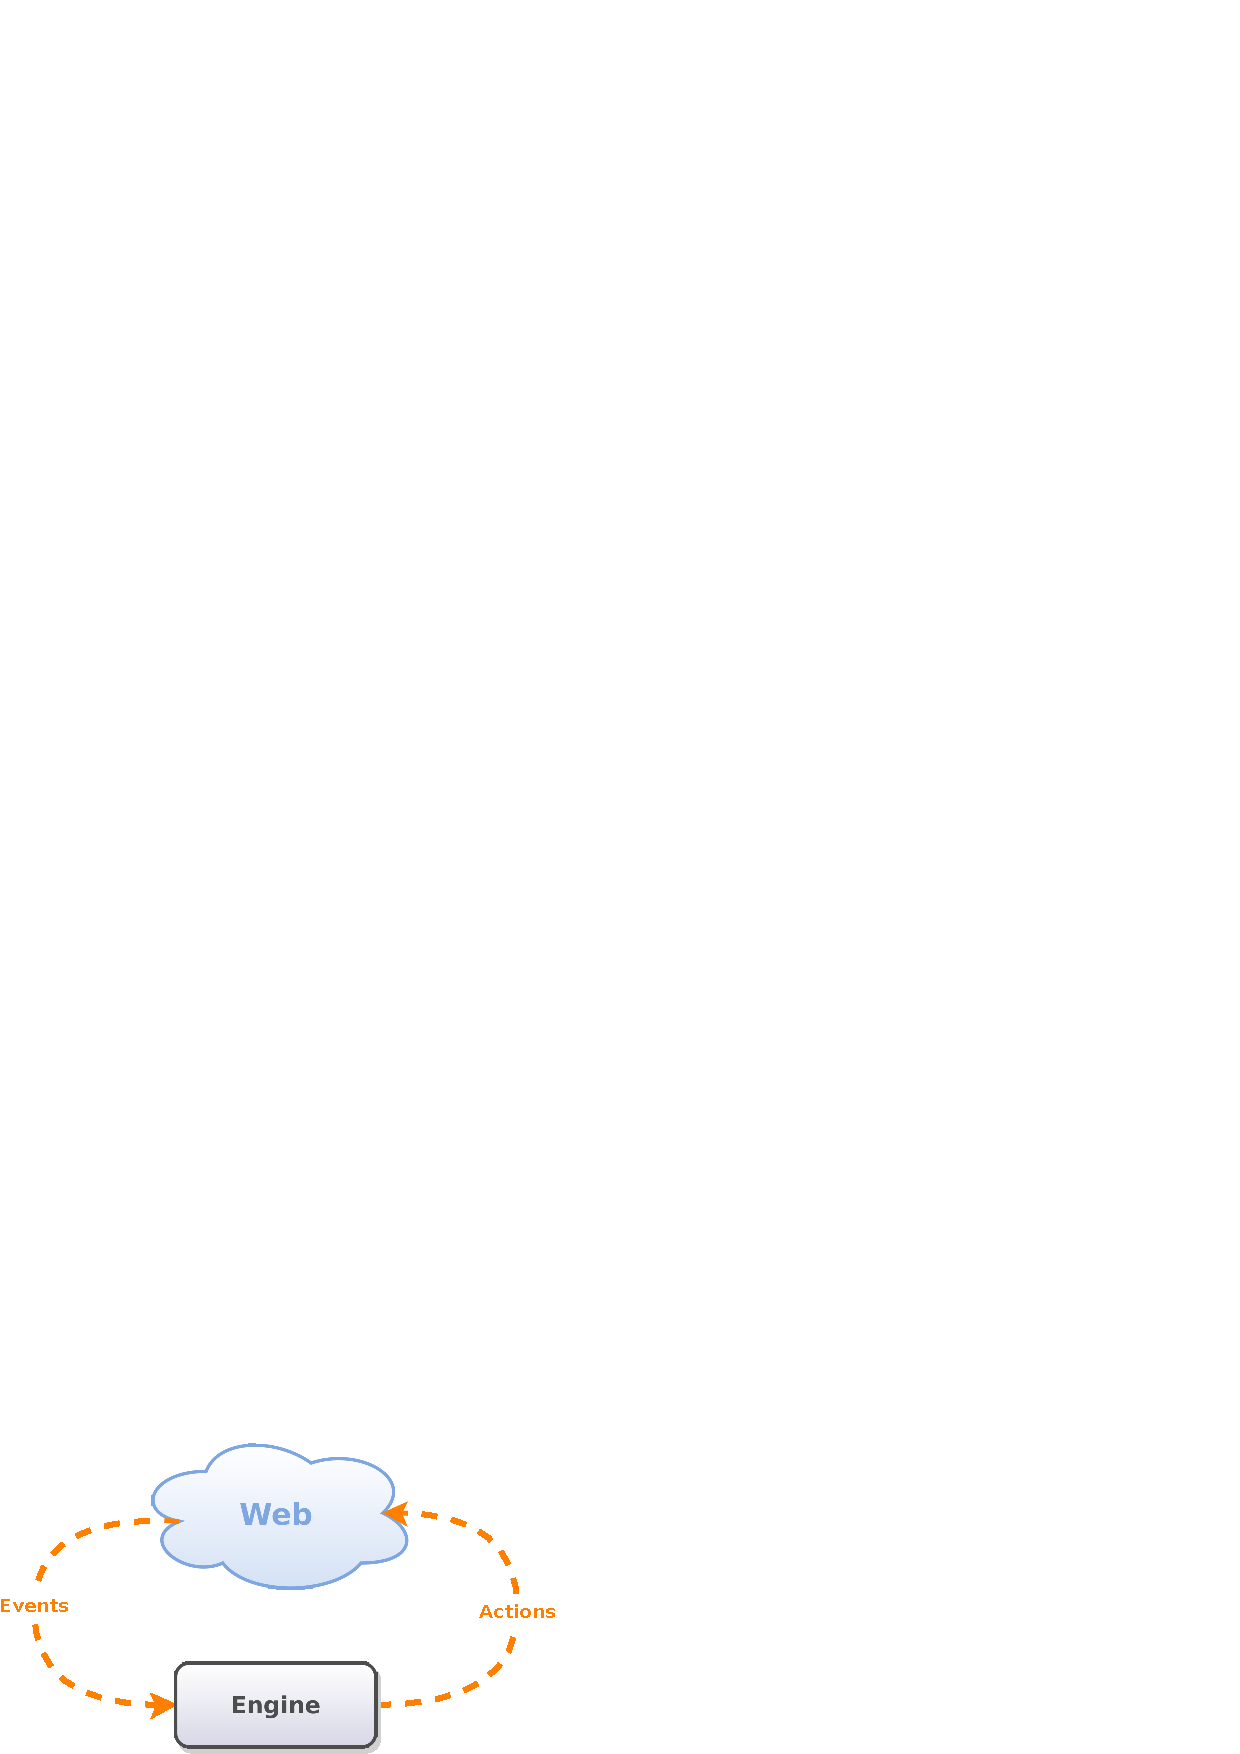
\includegraphics{figures/Conceptual_Model_Simple}
  \caption{Reactor ;) Conceptual model for reactive web systems}
  \label{fig:Conceptual_Model_Simple}
\end{figure}

\begin{figure}[!ht]
  \centering
  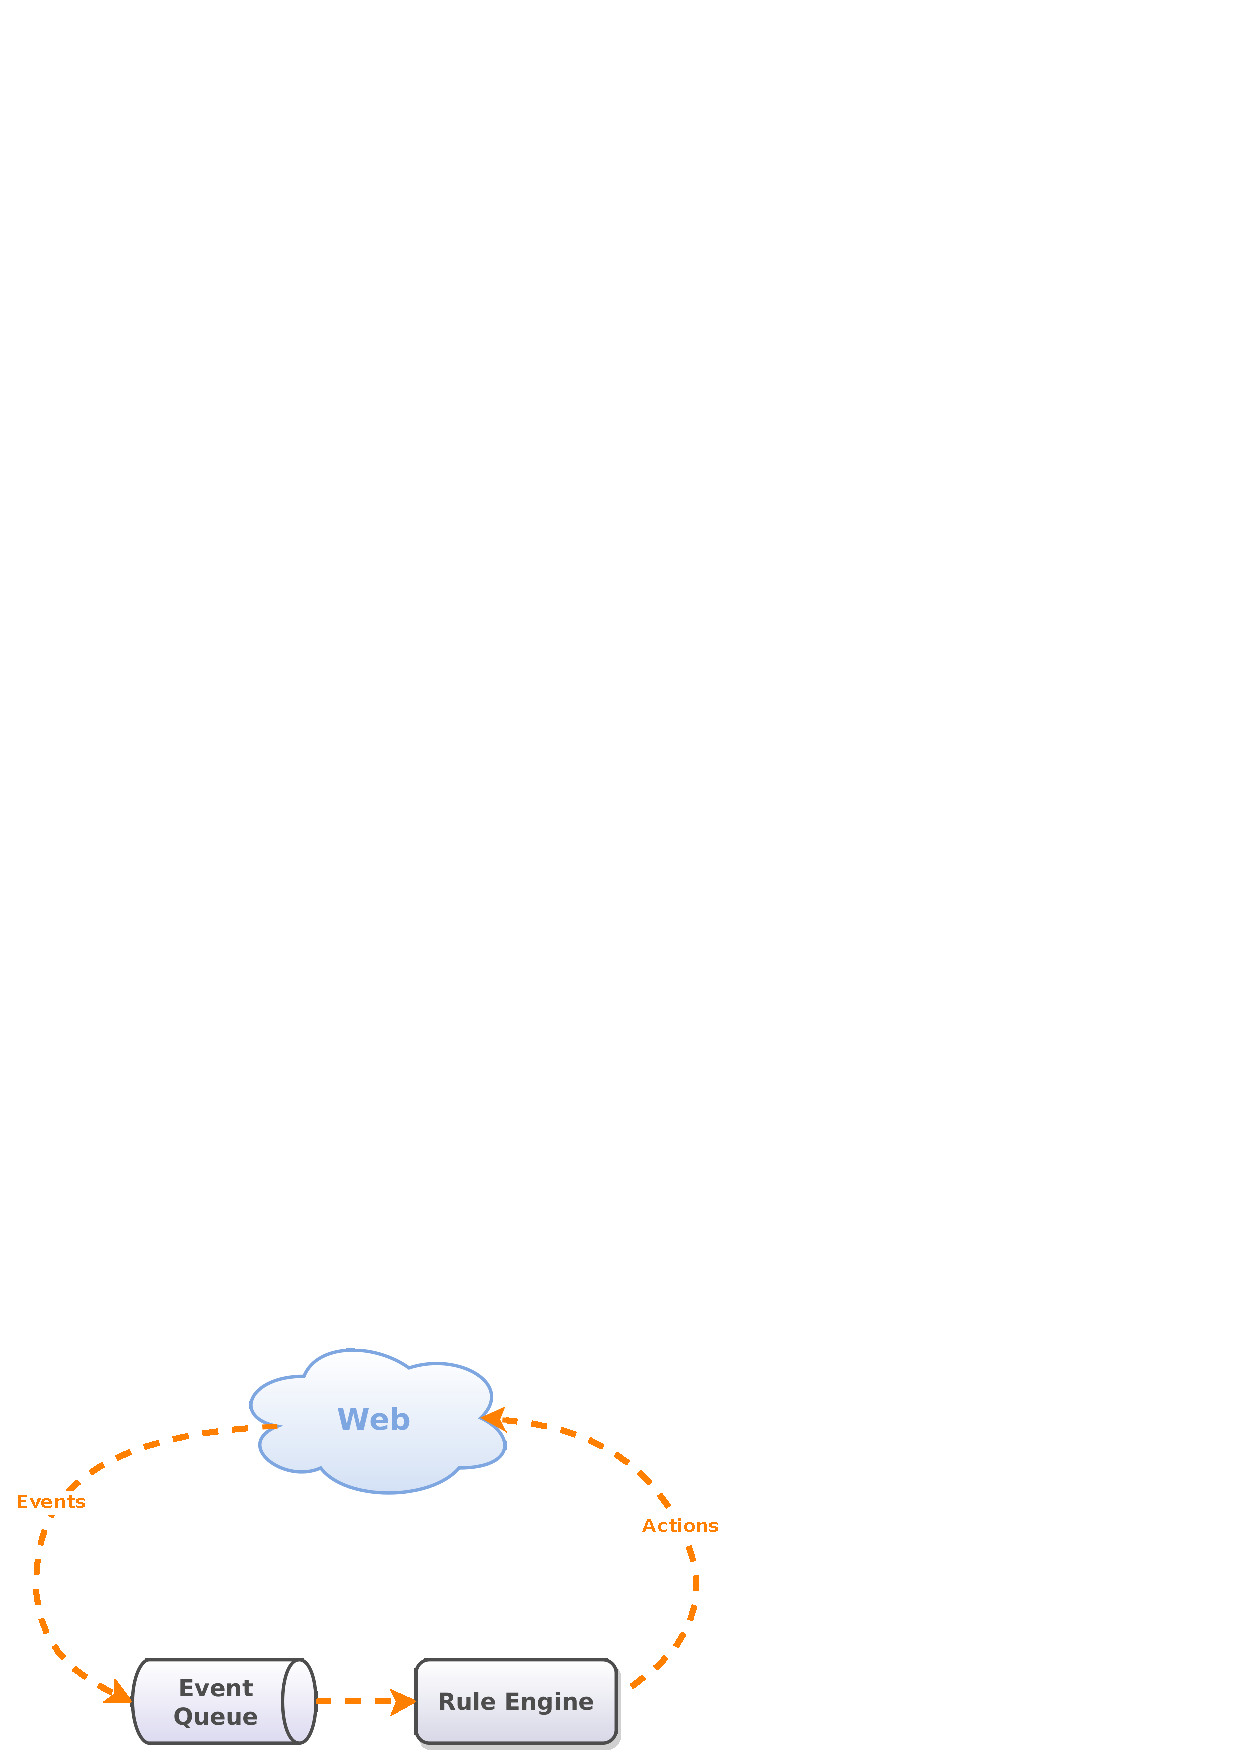
\includegraphics{figures/Conceptual_Model}
  \caption{Conceptual model for reactive Web Systems}
  \label{fig:Conceptual_Model}
\end{figure}


\begin{itemize}
  \item from web to events
  \item from events to rules
  \item from rules to actions
  \item from actions to the Web
  \item from concept to engine
\end{itemize}


% Regelimplementierungssprache
\subsection{Conceptual Rule Language}
Describe conceptual rule language
ON (existing categories)
IF (condition boundaries)
DO (call to existing action modules with parameters)

a lot possible, but dangerous.

\begin{Verbatim}[fontsize=\small,commandchars=\\\{\}]
\PY{k}{on} \PY{n}{mail}
\PY{k}{if} \PY{n}{sender}\PY{o}{=}\PY{l+s+ss}{\PYZdq{}sender@mail.com\PYZdq{}}
\PY{k}{do} \PY{n}{webapi}\PY{o}{\PYZhy{}}\PY{o}{\PYZgt{}}\PY{l+s+s2}{newcontent}\PY{p}{(}\PY{n}{subject}\PY{p}{)}
\end{Verbatim}

	\chapter{Applicability}
% informal description of target / story -> show that it makes sense
% Use Cases, not concrete
\section{Capturing the World-Wide Web}
\section{Capturing the Web of Things}
\section{Enhancing existing Web Applications}
\begin{itemize}
	\item Annotations
	\item Workflows Automation
	\item Availability and Functionality Testing
\end{itemize}
	

\chapter{Prototype System}
The prototype system is the adoption of our conceptual model for reactive \textrm{\glspl{infosystem}} and their services to the Web.
The Web consists of many \textrm{\glspl{infosystem}} and because of its \textrm{\acrlong{soa}} it can be seen as one large \textrm{\gls{infosystem}}, therefore we can impose reactivity on the Web.
Since communication over services in the Web is often latency driven, we came to the conclusion that asynchronous communication and therefore scalability should be attributes our prototype system has to support natively.
Another aspect to be regarded for the architectural decision was how the rules are going to be represented internally.
We introduced \textrm{\acrshort{xml}} and \textrm{\acrshort{json}} as common ways to communicate data between services on the Web.
Both formats represent data in a tree structure, and this is also what we decided to assume for the explicit parameters in the events that will enter our prototype.
Together with the requirement of native support for an \textrm{\acrlong{eda} (\acrshort{eda})} our decision was to build upon the recent adoption of \textrm{JavaScript} to application development through \textrm{Node.js}\footnote{http://nodejs.org/} and its human-readable \textrm{\acrshort{json}} communication format.

The prototype system consists of several modules, shown in Figure \ref{fig:Architecture}:
\begin{itemize}
	\item \textbf{\textrm{Poller}:} Loads \textrm{Event Trigger} modules and forwards events coming from them to the \textrm{Event Queue}. \textrm{Event Trigger} modules poll for changes in the Web and transform them into events. 
	\item \textbf{\textrm{Webhook Listener}:} Listens on active \textrm{Webhooks} for events and forwards them to the \textrm{Event Queue}.
	\item \textbf{\textrm{Event Queue}:} Buffers events for the case of an overly busy \textrm{Rule Engine}. 
	\item \textbf{\textrm{Rules Engine}:} Picks an event from the \textrm{Event Queue} whenever there is one and it is idle. 
	\item \textbf{\textrm{User Request Handler}:} The user interface modules to administrate \textrm{Event Trigger}, \textrm{Webhooks}, \textrm{Rules} and \textrm{Action Dispatchers}. A special case is the \textrm{Rules Administration} because it notifies the \textrm{Poller} and \textrm{Rules Engine} about new or updated Rules, which then in turn load required \textrm{Event Trigger} or \textrm{Action Dispatcher} modules.
\end{itemize}


a queue which receives all incoming events, and an engine that picks the events from the end of the queue whenever it is idle.
The engine checks the event against its stored ECA rules and fires the actions whenever a rule applies to an event.
When a new rule is stored, the engine instantiates the action modules that are required in case an event arrives at the system which triggers the actions.
The Web is a heterogeneous resource with many different types of systems and services, thus we can't rely on them for providing events to the webhooks of our system.
Thus we also implement the so called "event triggers" a way to pull events into our system through.
All they do is checking Web resources for changes and push events into the system whenever they detect one.
\begin{figure}[!ht]
	\centering
  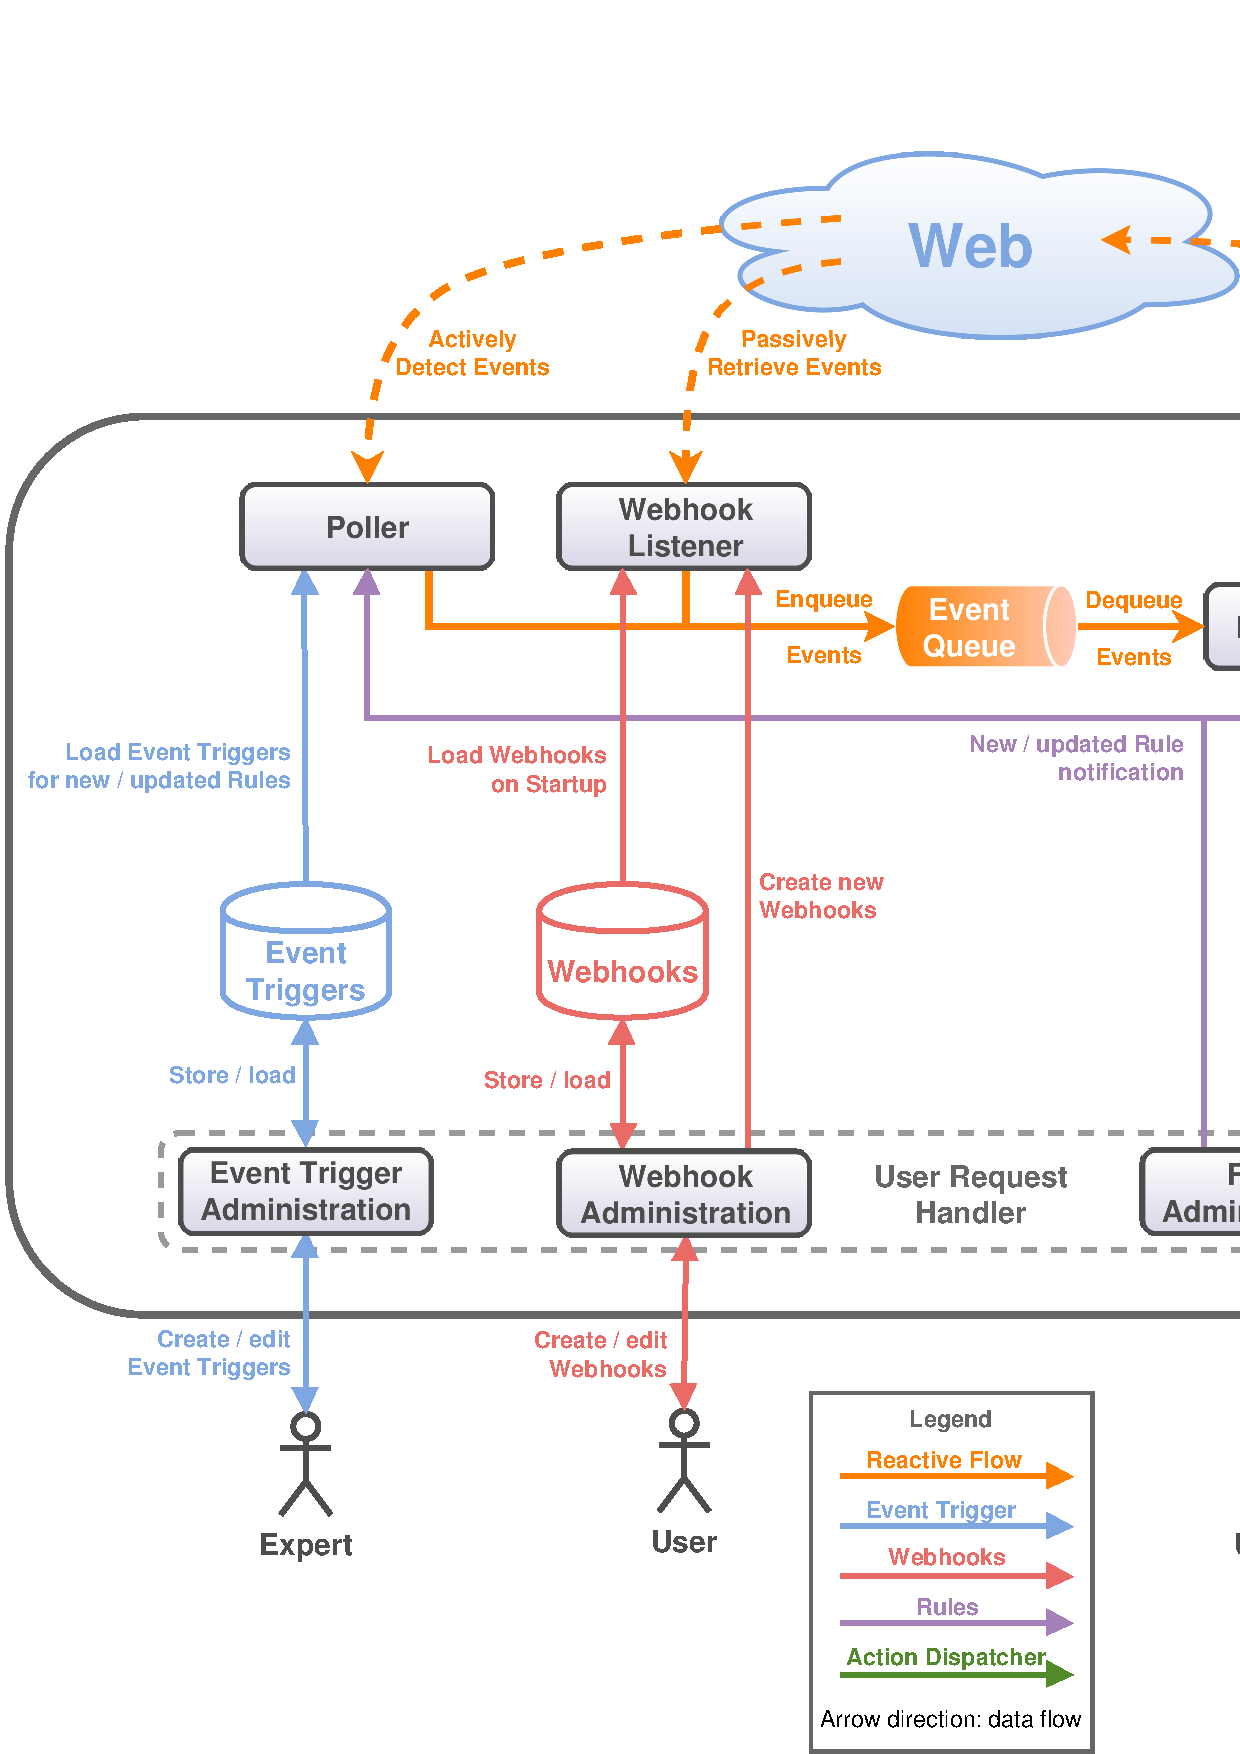
\includegraphics[width=\textwidth]{figures/Architecture_Final}
	\caption{Prototype System Architecture}
	\label{fig:Architecture}
\end{figure}



\section{Data Structure for Events}
Events in our prototype system are internally represented as tree structures in \textrm{\acrshort{json}} format, which builds on only two data structures:
\begin{itemize}
	\item Objects: Unordered collections of name/value pairs, which can also be implemented as a hash map, dictionary or struct in other languages.
	\item Arrays: Ordered lists of values, which can also be implemented as a record, vector or list in other languages.
\end{itemize}
A value can be an object or an array, but also a unicode string, a number, boolean or null.
This allows for any arbitrary depth and chaining of the supported data representations.
It is a handy feature when we assume a tree structure for events in our prototype system since the selection of nodes in tree structures has been well studied and useful libraries exist.
Since all native data structures within \textrm{JavaScript} programming code are already in \textrm{\acrshort{json}} format, it can easily be marshalled into one string and communicated to other applications without overhead.
\textrm{\acrshort{json}} can be implemented in virtually every programming language, therefore received a lot of attention and is supported by many \textrm{\glspl{webresource}} for communication.



% There's still the challenge of filtering
% What's important to whom
% Plus the user needs to have tools to combine and add programmability to the combination,( such as conditions, selection of provided arguments and so on)

% In the last section we showed how mashups create additional value for the Web by combining several Web API's.
% But it turned out, that such mashups are closed systems, which often only allow little degree of parametrization.

\section{Event Trigger}

% TODO Classify events in \textrm{\gls{infospace}}, information events: temperature, new mail, blabliblu
% TODO Classify Actions in \textrm{\gls{infospace}}


% Event Gathering is the E in ECA and without one of these letters such a system would not run.
% It is of utmost importance to find as much as possible ways to get data into a system.


% Preferably a lightweighted rules engine would be used to run the user-generated mashups. T

% NOTES / TODOs:
%
% Architecture scheme, implementation
% callback functions, hot plugin
% js-select selectors
% List of condition operators
% Why JS, why wasnt it used before? is it used now?
% Terminierungsproblem (compiler bau), loesungsansaetze


% as seen by user,
% as seen by developer


% \section{Architecture}


\subsection{Polling}


\subsection{Webhooks}
% we generate also events again to be pushed over webhooks, and also loopback events







\section{Action Dispatcher}
% Actions are functions that need to be predefined as in JSON Rules
% Through this it is possible to provide generic functions for expert user as well as very limited functions with only few possibilities for parameterization to be used by unexperienced persons.
% In our reasearch we focused mainly on server-sided \textrm{Web APIs}, even though we also generated events from the browser and pushed them into our prototype system and let
% But still since SOAP services are request responders they have their place in our model, both as event trigger and action invoker.
% We do not limit ourselves to protocols or architectures of services in the Web, but aim to access all of them in order to exploit the Web's full power.


% Not only from events
% import.io

\section{ECA Rules in the Engine}
% TODO Conditions

% describe internal loop
% Describe rule engine. start from real engine over graphic engine why do we call ours engine

% vague Rule language limited through user acounts to not harm the system
% Describe possible attacks
% is descriptive, adaptive, flexible

% Explain rules, transferrability to language?

% dynamic code modules to shield system from user modules

%explain modules and their properties / user associations




% Apply variable number of function arguments to function

% \section{Grab data from anywhere}

% TODO figure: Wer hat welche rollen?
% TODO figure: Event fluss in verschiedenen UCs
% TODO figure: event anomalien (3-4 knoten)
% TODO figure: Unterschied Push / Pull -> unter introduction bei Webhooks?

% Callbacks / Webhooks semantical similarities but at different layers





During our research we found a troublesome server room that shows how the \textrm{Web of Things} can be exposed through our model.
This server room suffered from a defective cooling system which lead to a drastical increase of temperature in certain circumstances.
As a consequence certain server automatically shut themselves down as safety measurements.
Eventually, these shutdowns weren't detected immediately by the people that administered these servers, therefore unnecessary downtimes were the result.
As a very quick fix to inform certain administrators about the shutdown of their server, we started pinging these servers and pushed the results int




We have also seen that virtual events have an implicit parameter which is the event name, thus this is the one that is referred to in the event part of a rule.
If an event name, of an event entering the \textrm{Rule Engine}, is detected in a predefined rule, the engine compares the event against the conditions of that rule and if all conditions are met, dispatches the actions defined within the rule.
\subsection{Rule Language for Reactive Information Systems}
We also assume that \textrm{Action Dispatcher} modules can be accessed through common function invocation syntax ( i.e. \texttt{actionFunction(param1, param2[, ...])} ) in order to dispatch an action to an \textrm{\gls{infosystem}}.
Through this we are able to define a rule language that uses tree node selectors in order to select explicit event parameters, which can then be verified against conditions and forwarded to \textrm{Action Dispatcher} modules as function parameters.
Listing \ref{lst:exampleRulePhrase} shows an example phrase of our envisioned rule language where the retrieval of a new mail will be checked for soccer news and, if confirmed, the mail body will be forwarded to an interested person.

\begin{lstlisting}[language=OwnRule,label={lst:exampleRulePhrase},caption=Example Phrase in Reactive Rule Language]
ON mailevent
IF #{ .subject } instr "Soccer News"
DO mail->send( "soccerfan@host.com", "News about soccer!", #{ .body } )
\end{lstlisting}


% ON (existing categories)
% IF (condition boundaries)
% DO (call to existing action modules with parameters)

% a lot possible, but dangerous.

% \begin{Verbatim}[fontsize=\small,commandchars=\\\{\}]
% \PY{k}{on} \PY{n}{mail}
% \PY{k}{if} \PY{n}{sender}\PY{o}{=}\PY{l+s+ss}{\PYZdq{}sender@mail.com\PYZdq{}}
% \PY{k}{do} \PY{n}{webapi}\PY{o}{\PYZhy{}}\PY{o}{\PYZgt{}}\PY{l+s+s2}{newcontent}\PY{p}{(}\PY{n}{subject}\PY{p}{)}
% \end{Verbatim}

% % TODO Define language with regular expression 
% % Programming language syntax is usually defined using a combination of regular expressions (for lexical structure) and Backus–Naur Form (for grammatical structure). Below is a simple grammar, based on Lisp:
% % expression ::= atom | list
% % atom       ::= number | symbol
% % number     ::= [+-]?['0'-'9']+
% % symbol     ::= ['A'-'Z''a'-'z'].*
% % list       ::= '(' expression* ')'
% \begin{lstlisting}[language=OwnRule,caption=Conceptual ECA Rule Language Syntax]
% expression  ::= 'on ' event ' if ' conditions ' do ' actions
% event       ::= symbol.*(' -> ' symbol.*)
% conditions  ::= 
% actions     ::= symbol*('('selector*')')
% symbol      ::= [A-Za-z0-9_-]+
% selector    ::= [#\{(symbol*?)\}]
% \end{lstlisting


% TODO Action Dispatcher
% Actions
% \begin{itemize}
%   \item Event Redirection
%   \item Event Enrichment
%   \item WebApp Actions
% \end{itemize}


% TODO conditions with examples
% TODO Imposing Acitons
% since we model changes in the data of an information space as events and actions, depending on wheter it is a read or wrtie action, we can impose reactivity to information systems.



% RL <-> ECA
% TODO figure: ECA Schema
% TODO Figure: ECA in the distributed environemnt
% TODO figure: Rules (unions / objects / Rueckkoppelungen )
% TODO engine




% Because of the heterogenous nature of the Web actions need to be abstracted
% as long as we do not limit ourselves e.g for RESTful access to services
% Describe conceptual rule language



% TODO concrete use case examples
\subsection{Example Use Cases}

% {
%     "dominic": {
%         "SOAP test": "{\"id\":\"SOAP test\",\"eventtype\":\"Custom Event\",\"eventname\":\"button-click\",\"conditions\":[],\"actions\":[\"SOAP -> convertCelsiusToFahrenheit\"]}",
%         "Presentation to Pushover": "{\"id\":\"Presentation to Pushover\",\"eventtype\":\"Custom Event\",\"eventname\":\"pushover\",\"conditions\":[],\"actions\":[\"Pushover -> broadcast\"]}",
%         "ProBinder Service Test: FAIL": "{\"id\":\"ProBinder Service Test: FAIL\",\"eventtype\":\"Custom Event\",\"eventname\":\"ProBinderServiceTest\",\"conditions\":[{\"selector\":\".success\",\"type\":\"bool\",\"operator\":\"==\",\"compare\":false}],\"actions\":[\"Pushover -> broadcast\",\"EMailYak -> sendMail\"]}",
%         "ProBinder Service Test": "{\"id\":\"ProBinder Service Test\",\"eventtype\":\"Event Poller\",\"eventname\":\"ProBinder Service Test -> testProBinder\",\"eventstart\":\"2014-05-20T13:00:00.000Z\",\"eventinterval\":120,\"conditions\":[],\"actions\":[\"System -> pushEvent\"],\"timestamp\":\"2014-05-20T11:51:46.307Z\"}",
%         "'button-click' Rule": "{\"id\":\"'button-click' Rule\",\"eventtype\":\"Custom Event\",\"eventname\":\"button-click\",\"conditions\":[],\"actions\":[\"Pushover -> broadcast\"]}",
%         "ProBinder annotate tags": "{\"id\":\"ProBinder annotate tags\",\"eventtype\":\"Event Poller\",\"eventname\":\"ProBinder -> unreadContent\",\"eventstart\":\"2014-05-20T19:11:00.000Z\",\"eventinterval\":1,\"conditions\":[],\"actions\":[\"ProBinder -> annotateTagEntries\",\"ProBinder -> setRead\"],\"timestamp\":\"2014-05-20T19:10:10.951Z\"}",
%         "Coffee Break": "{\"id\":\"Coffee Break\",\"eventtype\":\"Custom Event\",\"eventname\":\"uptimestatistics\",\"conditions\":[{\"selector\":\".currentlyon\",\"type\":\"value\",\"operator\":\">\",\"compare\":42}],\"actions\":[\"EMailYak -> sendMail\"]}",
%         "ProBinder Service Test: Logging": "{\"id\":\"ProBinder Service Test: Logging\",\"eventtype\":\"Custom Event\",\"eventname\":\"ProBinderServiceTest\",\"conditions\":[],\"actions\":[\"ProBinder -> newContent\"]}"
%     }
% }

\section{Web Programming}
% TODO find term in papers (full stack )


\subsection{Node.js}
% Why JS, why wasn't it used up to now? is it used now?

% http://benchmarksgame.alioth.debian.org/u64/benchmark.php?test=all&lang=java&lang2=v8&data=u64 seem to back our findings
% https://www.paypal-engineering.com/2013/11/22/node-js-at-paypal/ as well
% https://vividcortex.com/blog/2013/12/09/analysis-of-paypals-node-vs-java-benchmarks/ interpretes above results:
% My guess is that Node is encouraging good programmer practices in terms of scalability, and Java less so. In other words, programmers probably have to work less hard to avoid bad scalability bottlenecks in Node than in Java.

% TODO Take from preparation

% TODO figure: Callback; Result ensurance (ergebnissichherung) wird direkt mit funktion mitgeschickt

% Umgang mit der Zukunft
% Callback
\subsection{Callback Functions \& Asynchronous Closures}
% JAva futures? objekte für resultate sammeln

% NOTES / TODOs:
%
% Variable bindings
% Closures (https://developer.mozilla.org/en-US/docs/Web/JavaScript/Guide/Closures)$
% Closures are functions that refer to independent (free) variables. 
% In other words, the function defined in the closure 'remembers' the environment in which it was created in.

% write about arallel as well?

Often, optimization approaches and programming language concepts require special attention to avoid common pitfalls.
When closures are used as asynchronous functions, developers need to be very careful not to end up with race conditions.


Looking at an example of sequential code execution in Figure~\ref{fig:Closures_Synchronous}, we see that function execution of \texttt{fA} is halted until function \texttt{fB} is finished.
If \texttt{fB} happens to be a latency-driven I/O operation the completion of \texttt{fA} could be deferred for a relatively long time.
While the application waits for the completion of the I/O operation, some remaining operations in \texttt{fA} could eventually already be executed without causing any race conditions.
\begin{figure}[!ht]
	\centering
  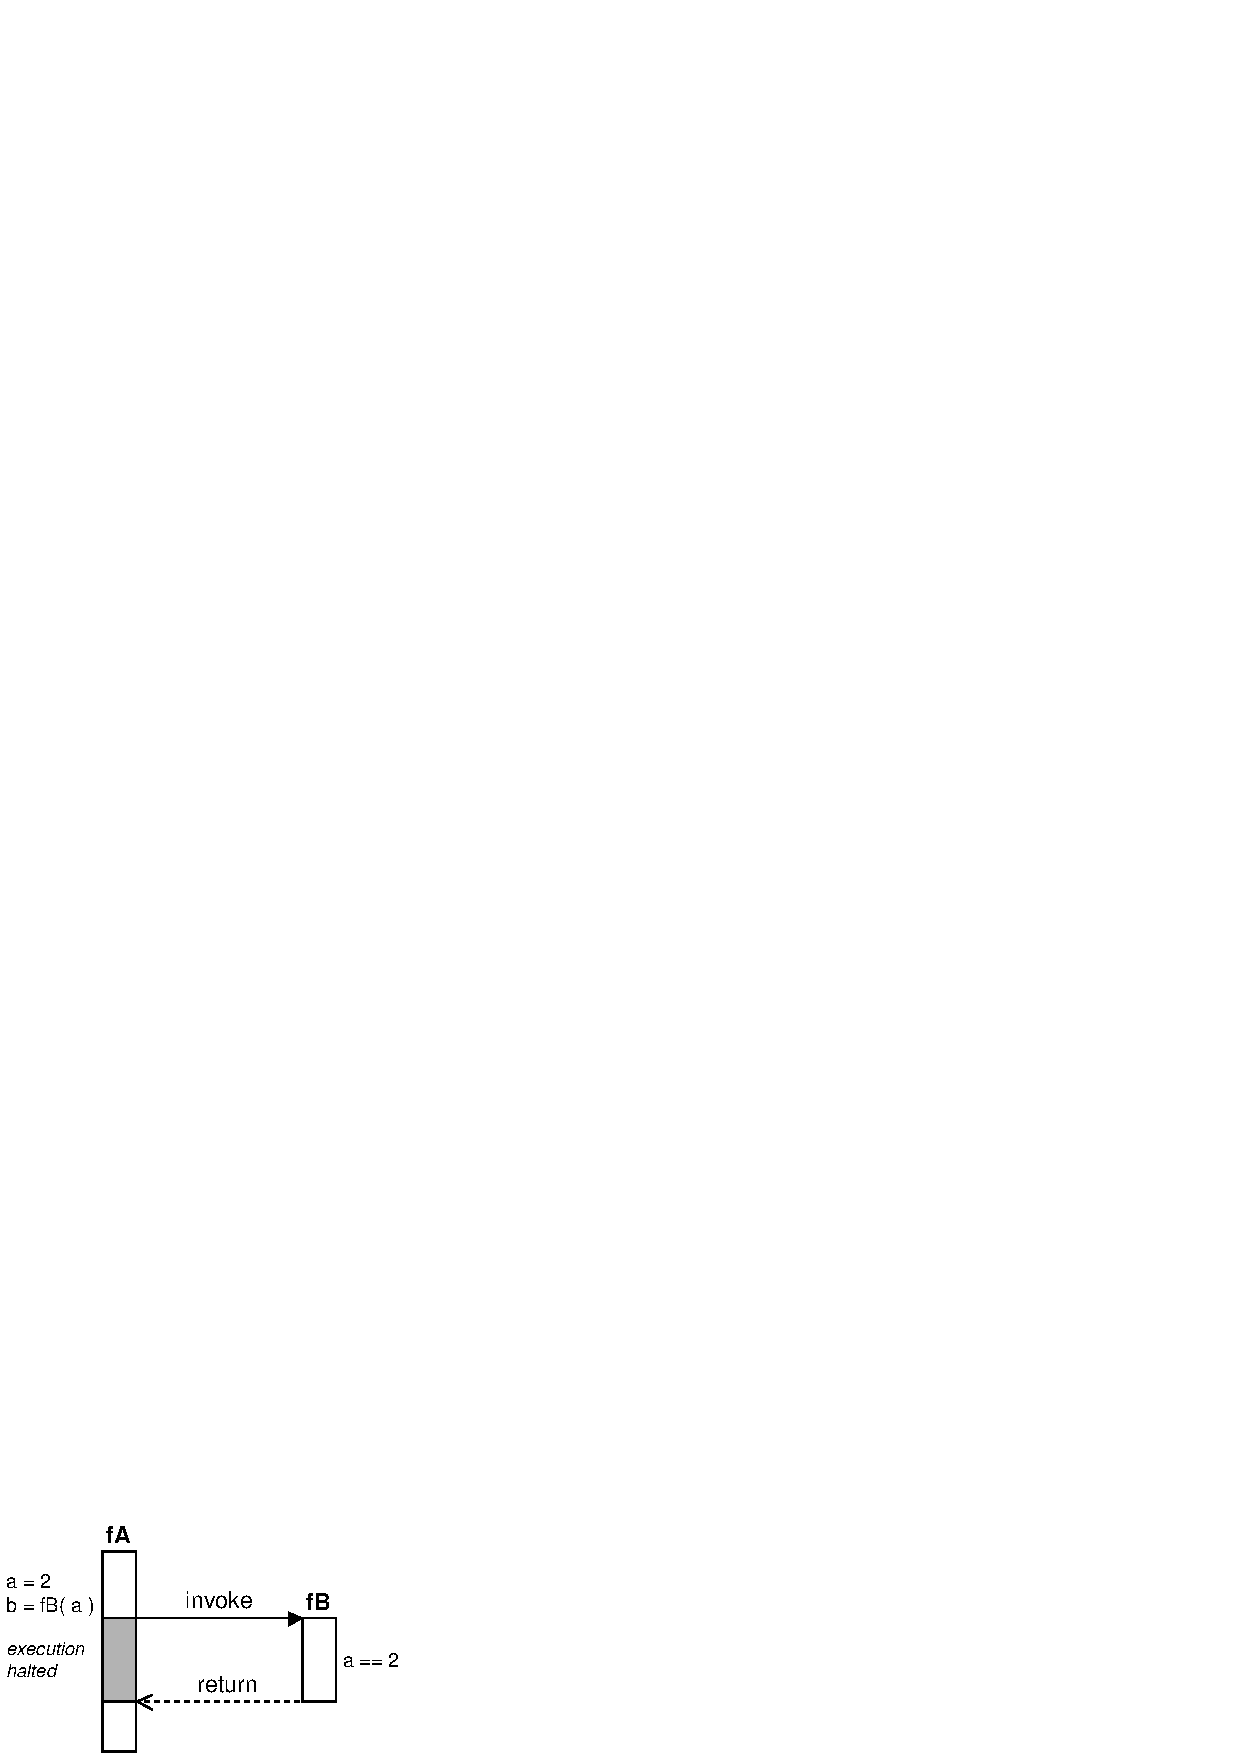
\includegraphics{figures/Closures_Synchronous}
	\caption{Synchronous Function Call}
	\label{fig:Closures_Synchronous}
\end{figure}

Asynchronous code execution, as shown in Figure~\ref{fig:Closures_Asynchronous}, allows non-blocking and thus scalable applications.
Non-blocking operations are a remedy for optimzed resource allocation and open up ways to overcome previously described unnecessary resource bindings.
Processing any kind of latency-driven I/O operation asynchronously ( e.g. filesystem access and socket communication ) exploits resources that would otherwise be bound while waiting for completion.
Such operations are processed and completed whenever required resources are available.
\begin{figure}[!ht]
	\centering
  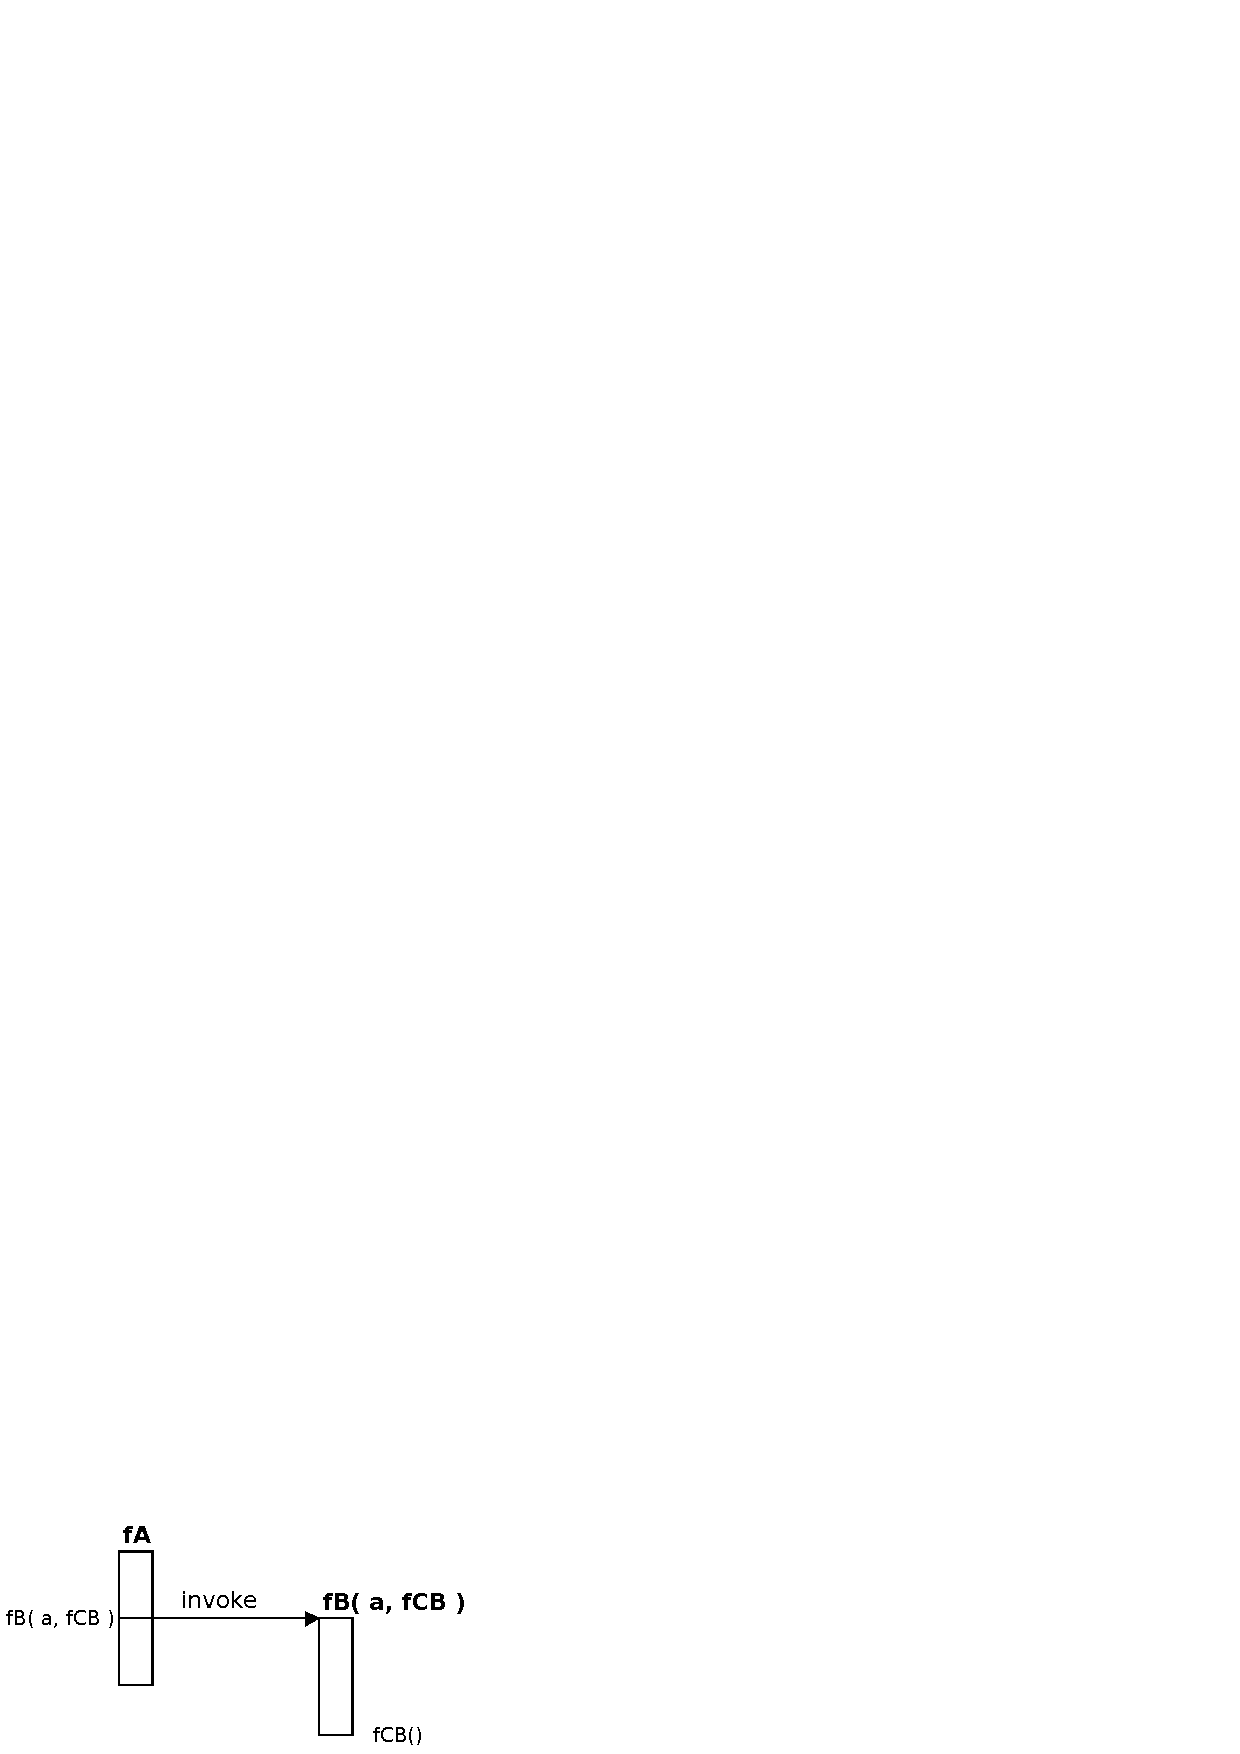
\includegraphics{figures/Closures_Asynchronous}
	\caption{Asynchronous Function Call}
	\label{fig:Closures_Asynchronous}
\end{figure}

Often other operations depend on the completion of asynchronous operations, hence their execution needs to be deferred.
This necessary code execution deferral is achieved through the use of callback functions, denoted \texttt{fCB} in Figure~\ref{fig:Closures_Asynchronous}.
Any code placed in a callback function, which is assigned to an asynchronous operation, is only executed after the respective asynchronous operation completed.
This allows stacking of functions and operations upon each other which automatically results in a flexible and event-driven application.

So far we didn't regard the context for such asynchronous functions.
If a function has access to the enclosing context where it was invoked in, it is called a closure.
Closures play an important role in ECMAScript\cite{EcmaScript}, which is the base for widely-spread script languages like JavaScript, JScript and ActionScript.
Closures in ECMAScript\cite{EcmaScript} are defined such as they have access to the context of the function they were created in.
This is shown in Figure~\ref{fig:Closures_Closure-1} where \texttt{c} from \texttt{fA}'s context is accessible from within \texttt{fB}, assuming that \texttt{fB} was created in \texttt{fA} and not only invoked from there.
Closures make it necessary for the context of the outer function to survive past its execution so no references are broken.
This is depicted through the "extended context lifetime" in Figure~\ref{fig:Closures_Closure-1}.
Using asynchronous closures it becomes evident, that the context in the invoking function can change while the closure is still computing and eventually referencing the outer context, thus causing race conditions.
This will be most obvious in a loop that immediately invokes \texttt{fB} several times, as shown in Figure~\ref{fig:Closures_Closure-2}.
In such a setup \texttt{c} will have different values in the same part of different invocations of \texttt{fB}.
\begin{figure}[!ht]
	\centering
  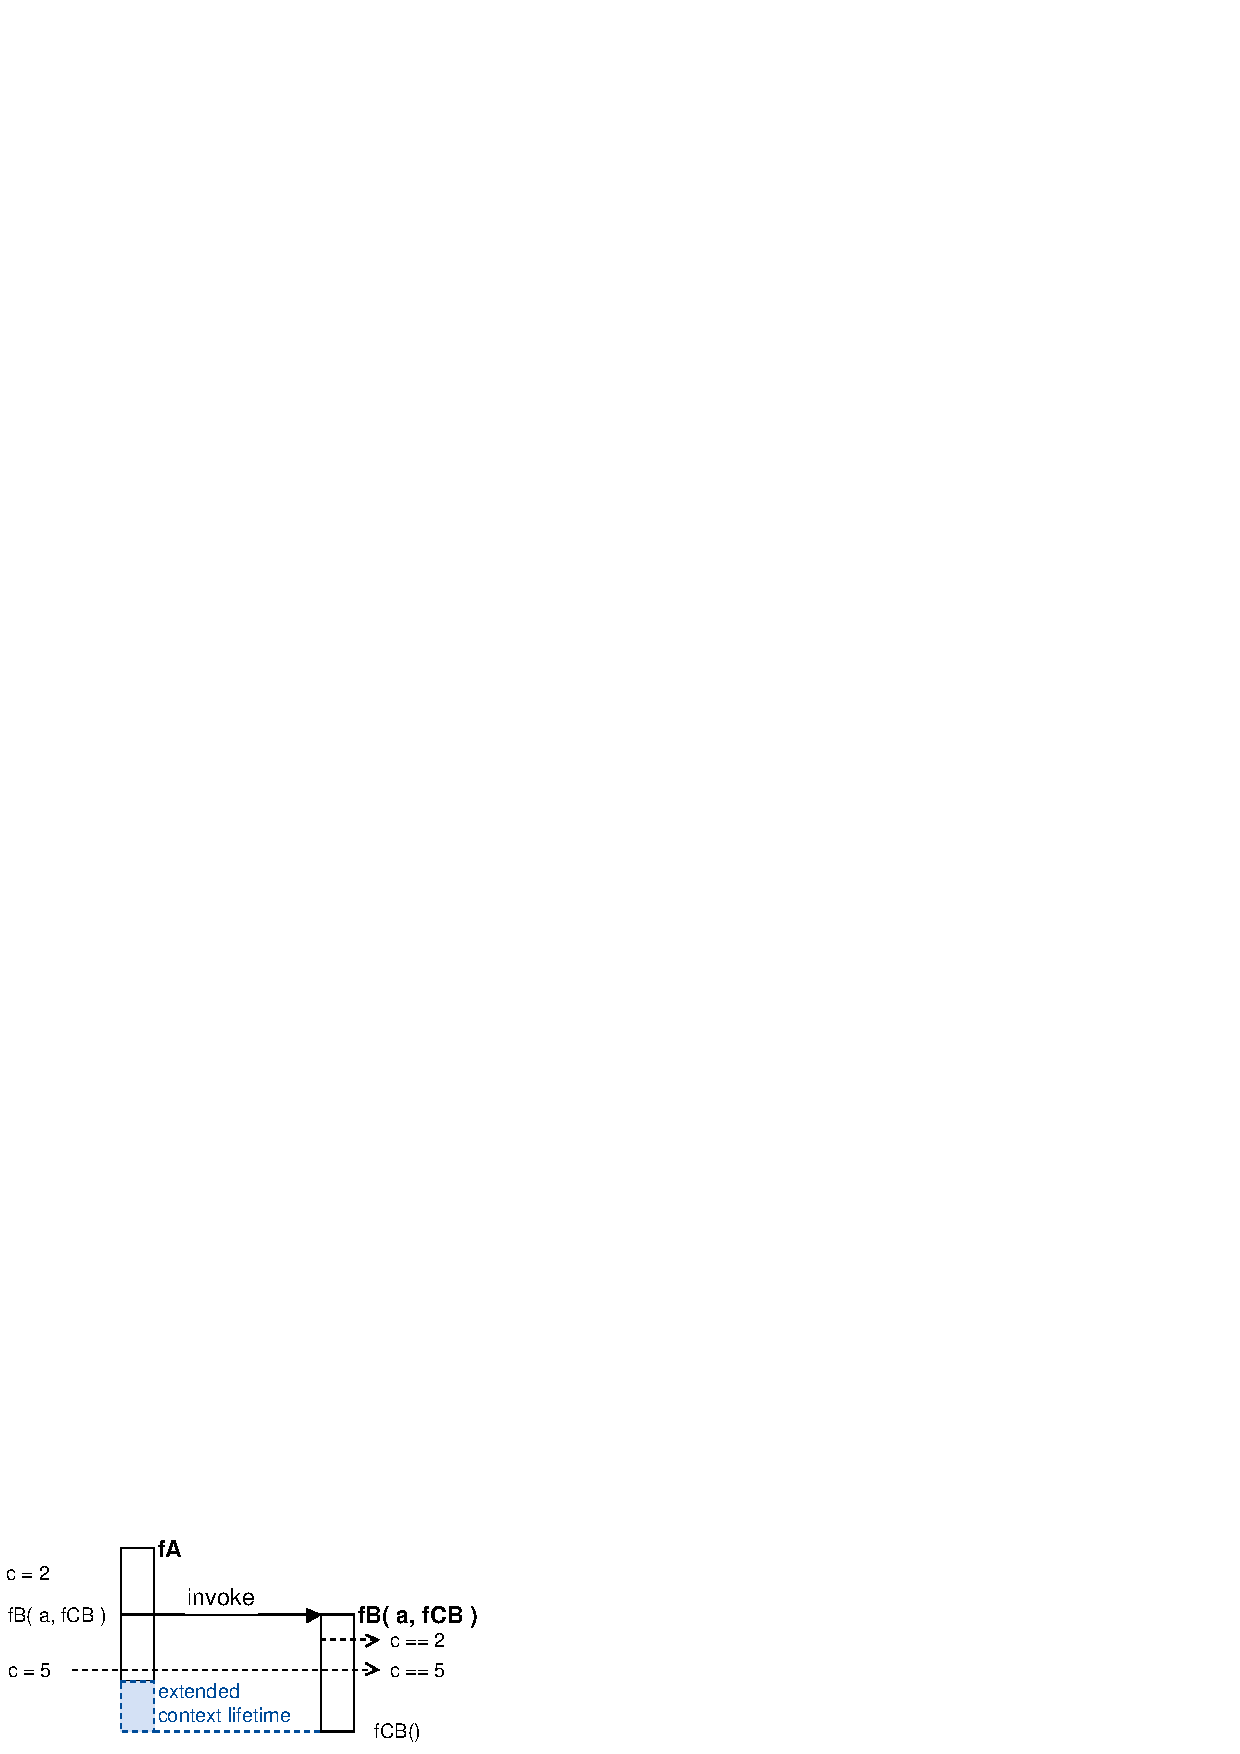
\includegraphics{figures/Closures_Closure-1}
	\caption{Closure Scope and referenced context}
	\label{fig:Closures_Closure-1}
\end{figure}
\begin{figure}[!ht]
	\centering
  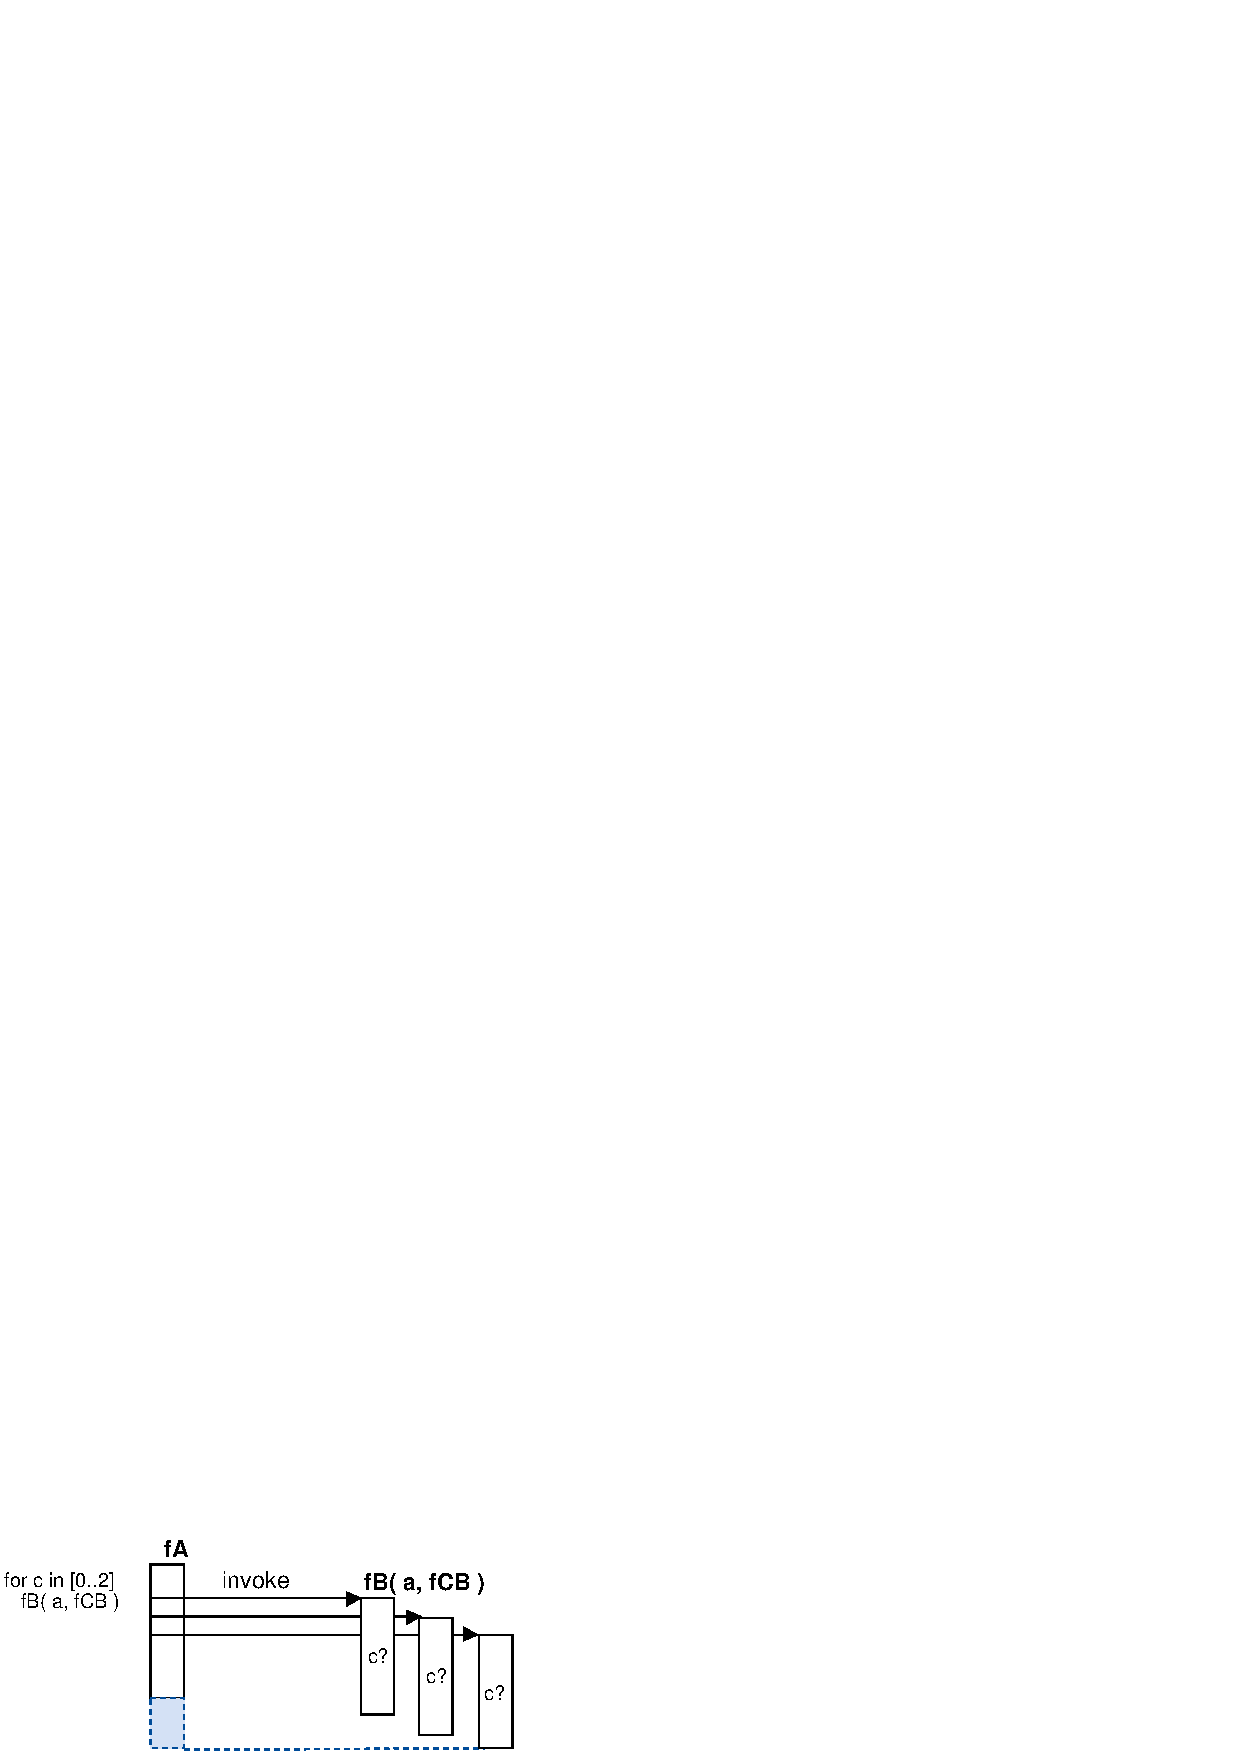
\includegraphics{figures/Closures_Closure-2}
	\caption{Closure context changes in a loop}
	\label{fig:Closures_Closure-2}
\end{figure}


Those event-driven context overwrites can be taken care of by shielding the closure from context changes, as shown in Figure~\ref{fig:Closures_Closure-3}.
To shield the closure form context changes, closure \texttt{fB} needs to create another closure \texttt{fC} and return it to \texttt{fA}.
The argument passed to \texttt{fB} is the context ( \texttt{c} in Figure~\ref{fig:Closures_Closure-3} ) that might change but requires to be persistent for one invocation.
\texttt{fC} has now \texttt{c} as a fixed context, which can't be overwritten anymore.
Now the only thing left is \texttt{fC} needs to be invoked and it will retain the original context.
This implementation is necessary when the closure acts as a callback function for asynchronous operations, to preserve the original context in case it is required within the callback function.
\begin{figure}[!ht]
	\centering
  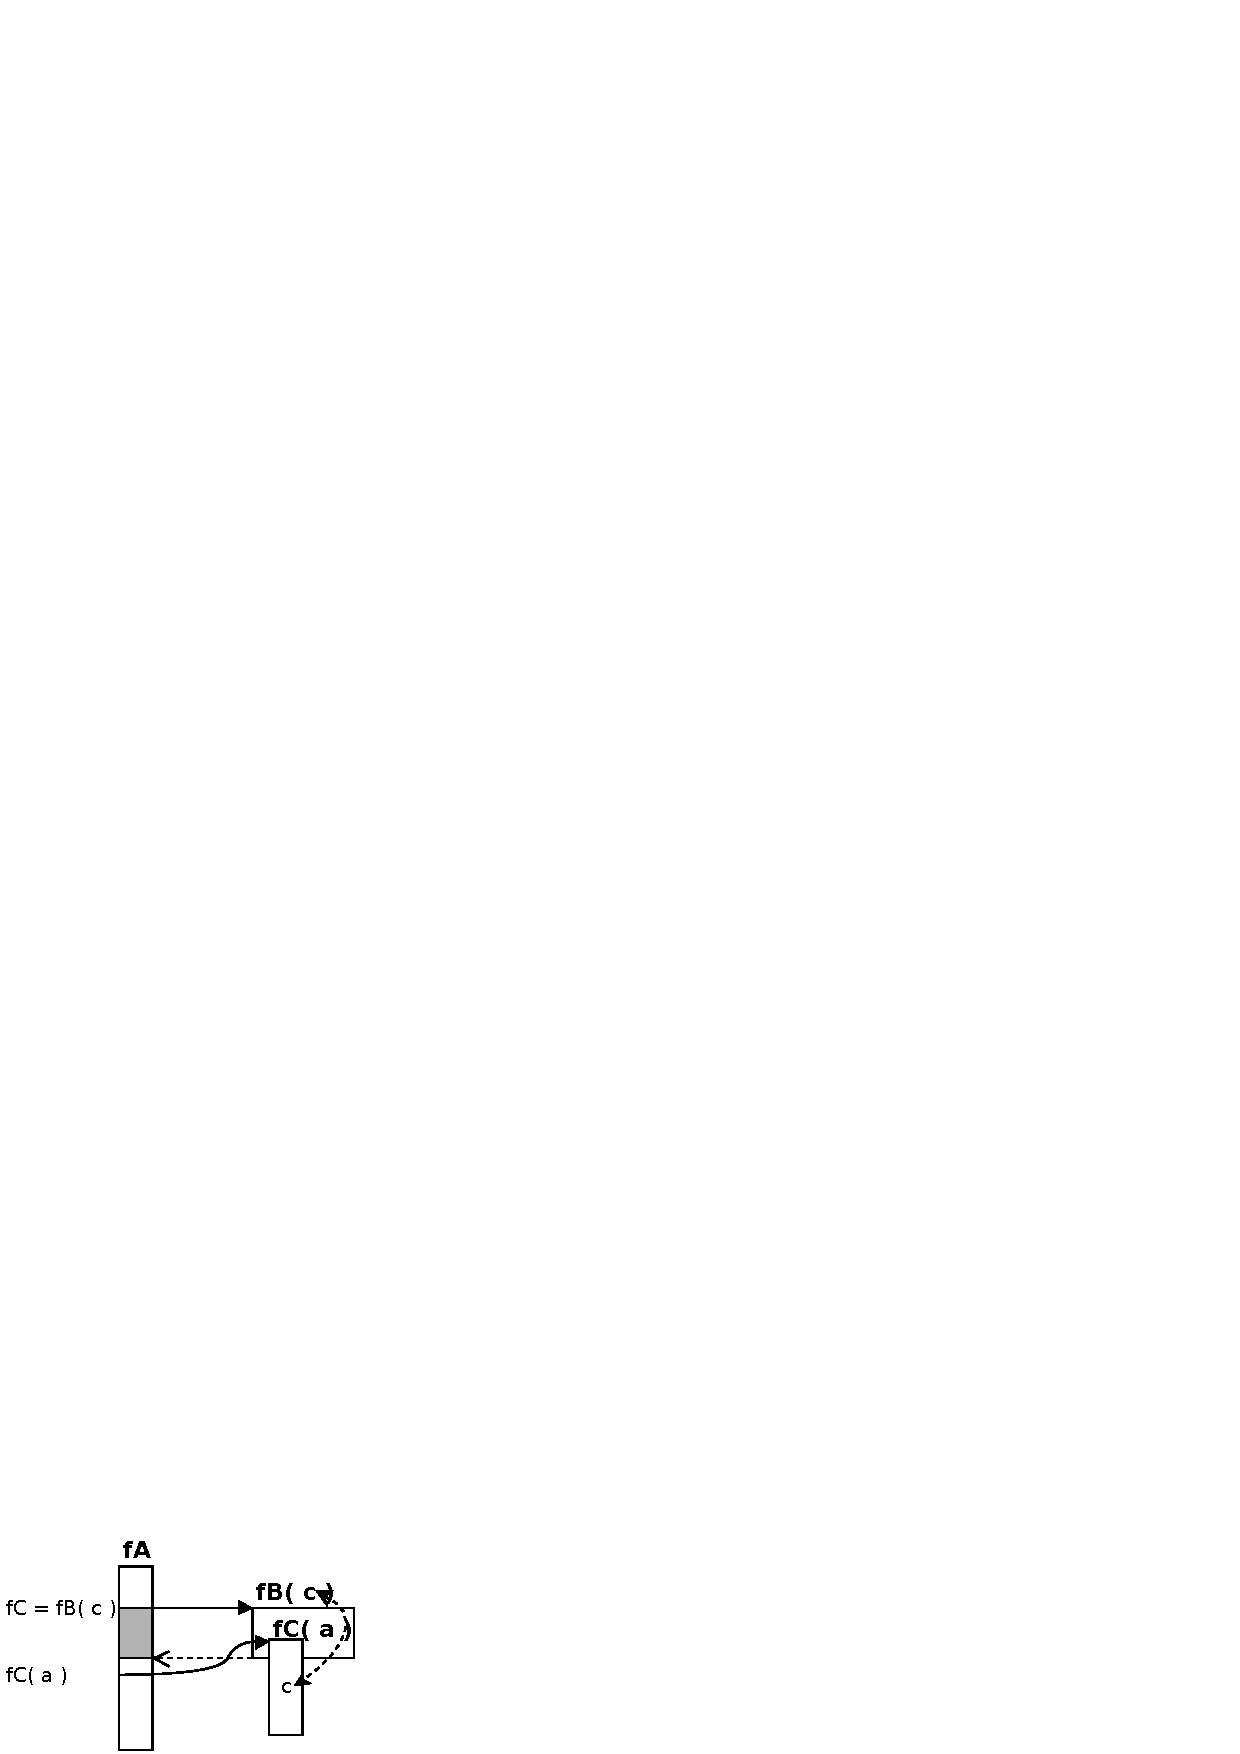
\includegraphics{figures/Closures_Closure-3}
	\caption{Closure Context Shielding}
	\label{fig:Closures_Closure-3}
\end{figure}

% TODO Figures need fA to be right aligned

An example of how closure contexts can be shielded is shown in the Listing \ref{lst_closure}.
\begin{lstlisting}[float=h,label=lst_closure,language=JavaScript,caption=JavaScript Context Shielding]
var fB = function( c ) { // Declare a function...
	var fC =  function( a ) { // ( <-- function to return )
		console.log( c );
	};
	return fC;
};
for( var c = 0; c < 100; c++ ) {
	// ... before you assign it to an event happening in the future:
	var fC = fB( c );
	setTimeout( fC, 3000); // will be executed after the loop ended
}
\end{lstlisting}

% TODO try async closures in other programming languages


% \subsubsection{Benchmarking JavaScript vs. Java}
% refer to listings
% TODO terminierungsproblem, testing, Web server, timeout, stacked callbacks.
%compilerbau?
%loesungsansätze?


% TODO why JS. JSON as first advantage (http://www.toptal.com/nodejs/why-the-hell-would-i-use-node-js)
% advantage for network applications with several concurrent connections
% not as client-server used as intented but as serverserver com since we also expect several connections simultanously under load.
% But also, we adopt the non-blocking nature of JS that is used for node's optimal communication, in order to implement our enigne in a non blocking way, thus allowing to load code and fire callback function in modules whenever they are required!
% http://ariya.ofilabs.com/2012/07/lazy-parsing-in-javascript-engines.html
% Optimization of special case if ( before function {immediately-invoked function expression (IIFE)}, do rela parsing, else lazy parsing
% Difference between context and scope. scope unique to each invocation, context is 'this', owner of currently executing code.
% .call, .apply 
% TODO we should use .bind for persistence.coffee's functions ....

%In JavaScript, functions are first-class objects, i.e. they are objects and can be manipulated and passed around just like any other object. Specifically, they are Function objects. -> https://developer.mozilla.org/en/docs/Web/JavaScript/Reference/Functions_and_function_scope
% Since each call provides potentially different arguments, a new closure is created for each call to outside. The memory can be freed only when the returned inside is no longer accessible

% The definitive guide: This combination of a function object and a scope (a set of variable bindings) in which the function’s variables are resolved is called a closure in the computer science literature.4
% This is an old term that refers to the fact that the function’s variables have bindings in the scope chain and that therefore the function is “closed over” its variables.


% Twelve Theses on Reactive Rules for the Web~\cite{10.1007-11896548_63}:
% This article investigates issues of relevance in designing high-level
% programming languages dedicated to reactivity on the Web. It presents
% twelve theses on features desirable for a language of reactive rules tuned
% to programming Web and Semantic Web applications.
% MY NOTES: they argue with soap and expect it to stay. They expect Web sites to inform each other about update requests. we are taking one step further and provide events to whomeever wants to receive them while being greedy about receiving events. give them to meeeeh my prciouzzz eventz!
% 1. High-level reactive languges are needed, ECA rules well-suited to specify reactivity
% 2. Reactive Web rules should be processed locally and act globally through event-based communication and access to persistent Web data
% 3. Events are best exchanged directly between Web sites in a push manner
% 4. Events are volatile data and should be kept distinct from persistent data.
% 5. Recognizing composite events is essential for a reactive Web language. Composite events are conveniently specified by (event) queries. There are (at least) four complementary dimensions to event queries: data extraction, event composition, temporal conditions, and event accumulation --> Future Work (CEP), data extraction already implemented
% 6. A data-driven, incremental evaluation of event queries is the approach of choice
% 7. Data from persistent Web resources plays an essential role for Web reactivity. A reactive language thus should embed or build upon a Web query language.
% 8. The Web is a dynamic, state-changing system. Reactions to state changes (events) through reactive rules are state-changing actions such as updates to persistent data. Reactive rules are needed where compound actions can be constructed from primitive actions.
% 9. Development and maintenance of reactive rule programs can be considerably supported by structuring mechanisms such as: branching in rules, deductive rules for event queries and Web queries, procedural abstractions for actions, and grouping of rules. --> Future work, attach several conditions and their actions branches to one event instead of creating rules for each of them. EC^nA^n. (Though procedural abstractions for actions already implemented, defining complex actions to be reused by rules)
% 10.Identity of data items is an issue for reactive languages due to their ability to react to changes of data objects on the Web. (we had surrogate identity though discarded the concept again... stupido)
% 11. Meta-programming and meta-circularity, that is, the ability to use rules to exchange and evaluate (other) rules, are needed in some important cases. (quite artificial for our scenarios)
% 12.Reactivity in the Web’s open and uncontrolled world requires language support for authentication, authorization, and accounting. (phew... let's let others go there)



% Tutorial example: as seen by user, as seen by the developer

	
\chapter{Conclusions \& Future Work}
% what reached, how to go on?
% Why is our system required, compare to servlets in terms of dynamic loading? user specific
% in the future what about somebody discovering our system as worthy to push events to? -> needs detection of new events
% We are taking a step further and allow not only the chaining up of several remote ECA engines, but also the invocation of actions on any arbitrary Web accessible service.

% In the future we could limit access to information systems to REST URI's and thus incorporate such calls into the language.
% but still we would need to be able to add logic, thus programming modules

%
% Temperature warning, using import.io
%http://khanlou.com/2014/03/model-view-whatever/
% Transactions in businesses, find use case. how would we lose events?
% Transactions for business. find use case.and explain how we would loose events.


% TODO Future Work
%
% CEP:

% Twelve Theses on Reactive Rules for the Web~\cite{10.1007-11896548_63}:
% This article investigates issues of relevance in designing high-level
% programming languages dedicated to reactivity on the Web. It presents
% twelve theses on features desirable for a language of reactive rules tuned
% to programming Web and Semantic Web applications.
% MY NOTES: they argue with soap and expect it to stay. They expect Web sites to inform each other about update requests. we are taking one step further and provide events to whomeever wants to receive them while being greedy about receiving events. give them to meeeeh my prciouzzz eventz!
% 1. High-level reactive languges are needed, ECA rules well-suited to specify reactivity
% 2. Reactive Web rules should be processed locally and act globally through event-based communication and access to persistent Web data
% 3. Events are best exchanged directly between Web sites in a push manner
% 4. Events are volatile data and should be kept distinct from persistent data.
% 5. Recognizing composite events is essential for a reactive Web language. Composite events are conveniently specified by (event) queries. There are (at least) four complementary dimensions to event queries: data extraction, event composition, temporal conditions, and event accumulation --> Future Work (CEP), data extraction already implemented
% 6. A data-driven, incremental evaluation of event queries is the approach of choice
% 7. Data from persistent Web resources plays an essential role for Web reactivity. A reactive language thus should embed or build upon a Web query language.
% 8. The Web is a dynamic, state-changing system. Reactions to state changes (events) through reactive rules are state-changing actions such as updates to persistent data. Reactive rules are needed where compound actions can be constructed from primitive actions.
% 9. Development and maintenance of reactive rule programs can be considerably supported by structuring mechanisms such as: branching in rules, deductive rules for event queries and Web queries, procedural abstractions for actions, and grouping of rules. --> Future work, attach several conditions and their actions branches to one event instead of creating rules for each of them. EC^nA^n. (Though procedural abstractions for actions already implemented, defining complex actions to be reused by rules)
% 10.Identity of data items is an issue for reactive languages due to their ability to react to changes of data objects on the Web. (we had surrogate identity though discarded the concept again... stupido)
% 11. Meta-programming and meta-circularity, that is, the ability to use rules to exchange and evaluate (other) rules, are needed in some important cases. (quite artificial for our scenarios)
% 12.Reactivity in the Web’s open and uncontrolled world requires language support for authentication, authorization, and accounting. (phew... let's let others go there)




% We have seen that the ECA approach is already a powerful one to make the Web reactive.
% CEP will result in an approach where events are not just processed when they are entering the system and evaluated against rules, but these events would need to be stored for quite a long time.
% Also the rules will not all be checked for each event but they are subject to a scheduler.
% It can be decided when and how often a rule is evaluated and all events will be checked at these point in times, whether they are candidates for firing the rule.
% A future improvement of this could be to adopt Complex Event Processing (CEP).
% This would mean that several events could be stored in a rule and be evaluated in terms of time constraints.
% Through this more complex events can be created as a result of several atomic events which would lead into semantically more complex events.


% TODO pathologische beispiele
% Endless loops -> child_process to be killed when not responding. what about async callbacks?

% Scheduler

% as long as we do not limit ourselves e.g for RESTful access to services we can't get it into a webquery language aight?

% RDFTL: The condition part is a query which de-
% termines if the information system is in a particular state, in which case the rule fires.

% TODO Condition evaluation on other resources? i.e. make a request to a remote site and evaluate it? -> also achievable through composite events
% Conditions evaluators could also be modules that are used to check certain states of information systems.
% Since we already have a lot of flexibility through our Event Triggers or Action Dispatchers this makes for us only sense for a future approach where CEP rules consist of accesses to REST interfaces, thus rule definitions get compiled into certain behaviour. such as web queries
% TODO Condition evaluation on other resources? i.e. make a request to a remote site and evaluate it? -> also achievable through composite events
% show rule engines, alsoo CEP, describe event composition through templates and why we don't do it

% automatic detection of new events within the system and information about them to the user
% the system needs to learn about events

% If we go to the semantic web we could incorporate RDF queries in order to allow smart event distinction

% web resurce (URI) can be data but also well defined service through REST. incorporating web resources into model 
% ince we're using URIs we could also set RDF logics on top of our event identification



% Bibliography
	\addcontentsline{toc}{chapter}{Bibliography}
	\bibliography{thesisbib}
	\bibliographystyle{thesisbst}

% Index
	\addcontentsline{toc}{chapter}{Index}
	\printindex

	% Turn off listing of tables and figures since from here on they will be in the appendix
	\captionsetup[figure]{list=no}
	\captionsetup[table]{list=no}

% Appendix
	\begin{appendices}
	\addtocontents{toc}{\setcounter{tocdepth}{-1}}
	
\chapter{Use Case Code}


\section{Node.js Code to ping IP Range and push the Result to a Remote Server\label{eventproducer}}

\begin{Verbatim}[fontsize=\scriptsize,commandchars=\\\{\},numbers=left,firstnumber=1,stepnumber=1]
\PY{c}{\PYZsh{} A node.js module to automatically ping an IP range and push the response result}
\PY{c}{\PYZsh{} to a remote server}

\PY{n}{fs} \PY{o}{=} \PY{n}{require} \PY{l+s}{\PYZdq{}}\PY{l+s}{fs}\PY{l+s}{\PYZdq{}}
\PY{n}{ping} \PY{o}{=} \PY{n}{require} \PY{l+s}{\PYZdq{}}\PY{l+s}{net\PYZhy{}ping}\PY{l+s}{\PYZdq{}}
\PY{n}{needle} \PY{o}{=} \PY{n}{require} \PY{l+s}{\PYZdq{}}\PY{l+s}{needle}\PY{l+s}{\PYZdq{}}
    
\PY{n}{remoteUrl} \PY{o}{=} \PY{l+s}{\PYZdq{}}\PY{l+s}{http://ec2\PYZhy{}54\PYZhy{}196\PYZhy{}2\PYZhy{}15.compute\PYZhy{}1.amazonaws.com}\PY{l+s}{\PYZdq{}}
\PY{n}{fPushEvent} \PY{o}{=} \PY{p}{(} \PY{n}{evt} \PY{p}{)} \PY{o}{\PYZhy{}}\PY{o}{\PYZgt{}}
  \PY{n}{needle}\PY{o}{.}\PY{n}{post} \PY{n}{remoteUrl} \PY{o}{+} \PY{l+s}{\PYZdq{}}\PY{l+s}{/measurements}\PY{l+s}{\PYZdq{}}\PY{p}{,} \PY{n}{JSON}\PY{o}{.}\PY{n}{stringify}\PY{p}{(} \PY{n}{evt} \PY{p}{)}\PY{p}{,} \PY{p}{(} \PY{n}{err}\PY{p}{,} \PY{n}{resp}\PY{p}{,} \PY{n}{body} \PY{p}{)} \PY{o}{\PYZhy{}}\PY{o}{\PYZgt{}}
    \PY{k}{if} \PY{n}{err} \PY{o+ow}{or} \PY{n}{resp}\PY{o}{.}\PY{n}{statusCode} \PY{n}{isnt} \PY{l+m+mi}{200}
      \PY{n}{console}\PY{o}{.}\PY{n}{log} \PY{l+s}{\PYZdq{}}\PY{l+s}{Error in pushing event!}\PY{l+s}{\PYZdq{}}
      \PY{n}{console}\PY{o}{.}\PY{n}{log} \PY{n}{err}
      \PY{n}{console}\PY{o}{.}\PY{n}{log} \PY{n}{resp}\PY{o}{.}\PY{n}{statusCode}
    \PY{k}{else}
      \PY{n}{console}\PY{o}{.}\PY{n}{log} \PY{l+s}{\PYZdq{}}\PY{l+s}{Successfully posted an event}\PY{l+s}{\PYZdq{}}

\PY{k}{try}
  \PY{n}{histData} \PY{o}{=} \PY{n}{fs}\PY{o}{.}\PY{n}{readFileSync} \PY{l+s}{\PYZdq{}}\PY{l+s}{histoappend.json}\PY{l+s}{\PYZdq{}}\PY{p}{,} \PY{l+s}{\PYZdq{}}\PY{l+s}{utf8}\PY{l+s}{\PYZdq{}}
\PY{n}{catch} \PY{n}{err}
  \PY{n}{console}\PY{o}{.}\PY{n}{error} \PY{n}{err}
  \PY{n}{console}\PY{o}{.}\PY{n}{error} \PY{l+s}{\PYZdq{}}\PY{l+s}{Error reading historical data file}\PY{l+s}{\PYZdq{}}
  \PY{n}{process}\PY{o}{.}\PY{n}{exit}\PY{p}{(}\PY{p}{)}

\PY{n}{session} \PY{o}{=} \PY{n}{ping}\PY{o}{.}\PY{n}{createSession} \PY{n}{retries}\PY{p}{:} \PY{l+m+mi}{2}
\PY{n}{oSum} \PY{o}{=} \PY{p}{\PYZob{}}\PY{p}{\PYZcb{}}
\PY{k}{if} \PY{n}{histData}
  \PY{n}{arrPings} \PY{o}{=} \PY{n}{histData}\PY{o}{.}\PY{n}{split} \PY{l+s}{\PYZdq{}}\PY{l+s+se}{\PYZbs{}n}\PY{l+s}{\PYZdq{}}
  \PY{k}{try}
    \PY{k}{for} \PY{n}{strObj}\PY{p}{,} \PY{n}{i} \PY{o+ow}{in} \PY{n}{arrPings}
      \PY{k}{if} \PY{n}{strObj} \PY{n}{isnt} \PY{l+s}{\PYZdq{}}\PY{l+s}{\PYZdq{}}
        \PY{n}{oTmp} \PY{o}{=} \PY{n}{JSON}\PY{o}{.}\PY{n}{parse} \PY{n}{strObj}  
        \PY{n}{oSum}\PY{p}{[} \PY{n}{oTmp}\PY{o}{.}\PY{n}{timestamp} \PY{p}{]} \PY{o}{=} 
          \PY{n+nb}{sum}\PY{p}{:} \PY{n}{oTmp}\PY{o}{.}\PY{n}{sum}
    \PY{k}{if} \PY{n}{oTmp}
      \PY{n}{fPushEvent}
        \PY{n}{currentlyon}\PY{p}{:} \PY{n}{oSum}\PY{p}{[} \PY{n}{oTmp}\PY{o}{.}\PY{n}{timestamp} \PY{p}{]}\PY{o}{.}\PY{n}{sum}
        \PY{n}{pingtimes}\PY{p}{:} \PY{n}{oSum}   

  \PY{n}{catch} \PY{n}{err}
    \PY{n}{console}\PY{o}{.}\PY{n}{log} \PY{l+s}{\PYZdq{}}\PY{l+s}{Error parsing histo data}\PY{l+s}{\PYZdq{}}
    \PY{n}{console}\PY{o}{.}\PY{n}{log} \PY{n}{err}

\PY{n}{i} \PY{o}{=} \PY{o}{\PYZhy{}}\PY{l+m+mi}{1}
\PY{n}{ips} \PY{o}{=} \PY{p}{[}\PY{p}{]}
\PY{n}{pingTime} \PY{o}{=} \PY{p}{(}\PY{n}{new} \PY{n}{Date}\PY{p}{(}\PY{p}{)}\PY{p}{)}\PY{o}{.}\PY{n}{toISOString}\PY{p}{(}\PY{p}{)}
\PY{n}{fPollHosts} \PY{o}{=} \PY{p}{(}\PY{p}{)} \PY{o}{\PYZhy{}}\PY{o}{\PYZgt{}}
  \PY{n}{session}\PY{o}{.}\PY{n}{pingHost} \PY{l+s}{\PYZdq{}}\PY{l+s}{192.168.1.\PYZsh{}\PYZob{} ++i \PYZcb{}}\PY{l+s}{\PYZdq{}}\PY{p}{,} \PY{p}{(} \PY{n}{err}\PY{p}{,} \PY{n}{target}\PY{p}{,} \PY{n}{sent}\PY{p}{,} \PY{n}{rcvd} \PY{p}{)} \PY{o}{\PYZhy{}}\PY{o}{\PYZgt{}}
    \PY{k}{if} \PY{o+ow}{not} \PY{n}{err}
      \PY{n}{ips}\PY{o}{.}\PY{n}{push} \PY{n}{target}
      
  \PY{k}{if} \PY{n}{i} \PY{o+ow}{is} \PY{l+m+mi}{255}
    \PY{n}{i} \PY{o}{=} \PY{o}{\PYZhy{}}\PY{l+m+mi}{1}
    \PY{n}{console}\PY{o}{.}\PY{n}{log} \PY{l+s}{\PYZdq{}\PYZdq{}\PYZdq{}}\PY{l+s}{\PYZsh{}\PYZob{} (new Date()).toISOString() \PYZcb{} | All ping requests returned (\PYZsh{}\PYZob{}ips.length\PYZcb{} answered),}
\PY{l+s}{      pushing event into the system and starting again at 0}\PY{l+s}{\PYZdq{}\PYZdq{}\PYZdq{}}
    
    \PY{n}{oSum}\PY{p}{[} \PY{n}{pingTime} \PY{p}{]} \PY{o}{=} \PY{n+nb}{sum}\PY{p}{:} \PY{n}{ips}\PY{o}{.}\PY{n}{length}
    \PY{n}{fPushEvent} \PY{n}{JSON}\PY{o}{.}\PY{n}{stringify}
      \PY{n}{currentlyon}\PY{p}{:} \PY{n}{ips}\PY{o}{.}\PY{n}{length}
      \PY{n}{pingtimes}\PY{p}{:} \PY{n}{oSum}

    \PY{n}{oPing} \PY{o}{=} 
      \PY{n}{timestamp}\PY{p}{:} \PY{n}{pingTime}
      \PY{n}{ips}\PY{p}{:} \PY{n}{ips}
      \PY{n+nb}{sum}\PY{p}{:} \PY{n}{ips}\PY{o}{.}\PY{n}{length}

    \PY{n}{fs}\PY{o}{.}\PY{n}{appendFile} \PY{l+s}{\PYZdq{}}\PY{l+s}{histoappend.json}\PY{l+s}{\PYZdq{}}\PY{p}{,} \PY{n}{JSON}\PY{o}{.}\PY{n}{stringify}\PY{p}{(} \PY{n}{oPing} \PY{p}{)} \PY{o}{+} \PY{l+s}{\PYZdq{}}\PY{l+s+se}{\PYZbs{}n}\PY{l+s}{\PYZdq{}}\PY{p}{,} \PY{l+s}{\PYZdq{}}\PY{l+s}{utf8}\PY{l+s}{\PYZdq{}}
    \PY{n}{pingTime} \PY{o}{=} \PY{p}{(}\PY{n}{new} \PY{n}{Date}\PY{p}{(}\PY{p}{)}\PY{p}{)}\PY{o}{.}\PY{n}{toISOString}\PY{p}{(}\PY{p}{)}
    \PY{n}{ips} \PY{o}{=} \PY{p}{[}\PY{p}{]}

  \PY{n}{setTimeout} \PY{n}{fPollHosts}\PY{p}{,} \PY{l+m+mi}{7000}

\PY{n}{fPollHosts}\PY{p}{(}\PY{p}{)}
\end{Verbatim}






\clearpage
\section{Coffee Break Invitation Rule object \label{ruleCoffeeBreak}}

\begin{Verbatim}[samepage=true,frame=single,fontsize=\footnotesize,commandchars=\\\{\},numbers=left,firstnumber=1,stepnumber=1,xleftmargin
=.3in]
\PY{p}{\PYZob{}}
  \PY{n+nt}{\PYZdq{}eventname\PYZdq{}}\PY{p}{:} \PY{l+s+s2}{\PYZdq{}uptimestatistics\PYZdq{}}\PY{p}{,}
  \PY{n+nt}{\PYZdq{}conditions\PYZdq{}}\PY{p}{:} \PY{p}{[}
    \PY{p}{\PYZob{}}
      \PY{n+nt}{\PYZdq{}selector\PYZdq{}}\PY{p}{:} \PY{l+s+s2}{\PYZdq{}.currentlyon\PYZdq{}}\PY{p}{,}
      \PY{n+nt}{\PYZdq{}operator\PYZdq{}}\PY{p}{:} \PY{l+s+s2}{\PYZdq{}\PYZgt{}\PYZdq{}}\PY{p}{,}
      \PY{n+nt}{\PYZdq{}compare\PYZdq{}}\PY{p}{:} \PY{l+m+mi}{42}
    \PY{p}{\PYZcb{}}
  \PY{p}{]}\PY{p}{,}
  \PY{n+nt}{\PYZdq{}actions\PYZdq{}}\PY{p}{:} \PY{p}{[}
    \PY{l+s+s2}{\PYZdq{}EMailYak \PYZhy{}\PYZgt{} sendMail(\PYZbs{}\PYZdq{}eca\PYZhy{}engine@mscliveweb.simpleyak.com\PYZbs{}\PYZdq{},[usermaillist],}
\PY{l+s+s2}{      \PYZbs{}\PYZdq{}Coffee Break!\PYZbs{}\PYZdq{},\PYZbs{}\PYZdq{}Let\PYZsq{}s go for a coffee at 10!\PYZbs{}\PYZdq{})\PYZdq{}}
  \PY{p}{]}
\PY{p}{\PYZcb{}}
\end{Verbatim}



\section{ProBinder Annotation Rule in JSON Format \label{ruleAnnotation}}
\begin{Verbatim}[samepage=true,frame=single,fontsize=\footnotesize,commandchars=\\\{\},numbers=left,firstnumber=1,stepnumber=1,xleftmargin
=.3in]
\PY{p}{\PYZob{}}
  \PY{n+nt}{\PYZdq{}eventname\PYZdq{}}\PY{p}{:} \PY{l+s+s2}{\PYZdq{}ProBinder \PYZhy{}\PYZgt{} unreadContent\PYZdq{}}\PY{p}{,}
  \PY{n+nt}{\PYZdq{}conditions\PYZdq{}}\PY{p}{:} \PY{p}{[}
    \PY{p}{\PYZob{}}
    \PY{n+nt}{\PYZdq{}selector\PYZdq{}}\PY{p}{:} \PY{l+s+s2}{\PYZdq{}.context .id\PYZdq{}}\PY{p}{,}
    \PY{n+nt}{\PYZdq{}operator\PYZdq{}}\PY{p}{:} \PY{l+s+s2}{\PYZdq{}==\PYZdq{}}\PY{p}{,}
    \PY{n+nt}{\PYZdq{}compare\PYZdq{}}\PY{p}{:} \PY{l+m+mi}{18749}
    \PY{p}{\PYZcb{}}
  \PY{p}{]}\PY{p}{,}
  \PY{n+nt}{\PYZdq{}actions\PYZdq{}}\PY{p}{:} \PY{p}{[}
    \PY{l+s+s2}{\PYZdq{}ProBinder \PYZhy{}\PYZgt{} annotateTagEntries(\PYZbs{}\PYZdq{}\PYZsh{}\PYZob{} .id \PYZcb{}\PYZbs{}\PYZdq{})\PYZdq{}} \PY{p}{,}
    \PY{l+s+s2}{\PYZdq{}ProBinder \PYZhy{}\PYZgt{} setRead(\PYZbs{}\PYZdq{}\PYZsh{}\PYZob{} .id \PYZcb{}\PYZbs{}\PYZdq{})\PYZdq{}}
  \PY{p}{]}
\PY{p}{\PYZcb{}}
\end{Verbatim}





\clearpage
\section{ProBinder Event Trigger\label{pbeventpoller}}
\begin{Verbatim}[fontsize=\scriptsize,commandchars=\\\{\},numbers=left,firstnumber=1,stepnumber=1]
\PY{c}{\PYZsh{} \PYZsh{}\PYZsh{}\PYZsh{} }
\PY{c}{\PYZsh{} ProBinder EVENT POLLER}
\PY{c}{\PYZsh{} \PYZhy{}\PYZhy{}\PYZhy{}\PYZhy{}\PYZhy{}\PYZhy{}\PYZhy{}\PYZhy{}\PYZhy{}\PYZhy{}\PYZhy{}\PYZhy{}\PYZhy{}\PYZhy{}\PYZhy{}\PYZhy{}\PYZhy{}\PYZhy{}\PYZhy{}\PYZhy{}\PYZhy{}\PYZhy{}}

\PY{c}{\PYZsh{} Global variables}
\PY{c}{\PYZsh{} This module requires user\PYZhy{}specific parameters:}

\PY{c}{\PYZsh{} \PYZhy{} username}
\PY{c}{\PYZsh{} \PYZhy{} password}
\PY{c}{\PYZsh{} \PYZsh{}\PYZsh{}\PYZsh{}}
\PY{n}{urlService} \PY{o}{=} \PY{l+s}{\PYZsq{}}\PY{l+s}{https://probinder.com/service/}\PY{l+s}{\PYZsq{}}
\PY{n}{credentials} \PY{o}{=}
  \PY{n}{username}\PY{p}{:} \PY{n}{params}\PY{o}{.}\PY{n}{username}
  \PY{n}{password}\PY{p}{:} \PY{n}{params}\PY{o}{.}\PY{n}{password}

\PY{c}{\PYZsh{}}
\PY{c}{\PYZsh{} The standard callback can be used if callback is not provided, e.g. if}
\PY{c}{\PYZsh{} the function is called from outside}
\PY{c}{\PYZsh{}}
\PY{n}{standardCallback} \PY{o}{=} \PY{p}{(} \PY{n}{funcName} \PY{p}{)} \PY{o}{\PYZhy{}}\PY{o}{\PYZgt{}}
  \PY{p}{(} \PY{n}{err}\PY{p}{,} \PY{n}{resp}\PY{p}{,} \PY{n}{body} \PY{p}{)} \PY{o}{\PYZhy{}}\PY{o}{\PYZgt{}}
    \PY{k}{if} \PY{n}{err}
      \PY{n}{log} \PY{l+s}{\PYZdq{}}\PY{l+s}{ERROR: During function }\PY{l+s}{\PYZsq{}}\PY{l+s}{\PYZsh{}\PYZob{} funcName \PYZcb{}}\PY{l+s}{\PYZsq{}}\PY{l+s}{\PYZdq{}}
    \PY{k}{else}
      \PY{k}{if} \PY{n}{resp}\PY{o}{.}\PY{n}{statusCode} \PY{o+ow}{is} \PY{l+m+mi}{200}
        \PY{n}{log} \PY{l+s}{\PYZdq{}}\PY{l+s}{Function }\PY{l+s}{\PYZsq{}}\PY{l+s}{\PYZsh{}\PYZob{} funcName \PYZcb{}}\PY{l+s}{\PYZsq{}}\PY{l+s}{ ran through without error}\PY{l+s}{\PYZdq{}}
      \PY{k}{else}
        \PY{n}{log} \PY{l+s}{\PYZdq{}}\PY{l+s}{ERROR: During function }\PY{l+s}{\PYZsq{}}\PY{l+s}{\PYZsh{}\PYZob{} funcName \PYZcb{}}\PY{l+s}{\PYZsq{}}\PY{l+s}{: \PYZsh{}\PYZob{} body.error.message \PYZcb{}}\PY{l+s}{\PYZdq{}}

\PY{c}{\PYZsh{} \PYZsh{}\PYZsh{}\PYZsh{}}
\PY{c}{\PYZsh{} Call the ProBinder service with the given parameters.}

\PY{c}{\PYZsh{}  \PYZhy{} \PYZob{}Object\PYZcb{} args the required function arguments object}
\PY{c}{\PYZsh{}  \PYZhy{} \PYZob{}Object\PYZcb{} [args.data] the data to be posted}
\PY{c}{\PYZsh{}  \PYZhy{} \PYZob{}String\PYZcb{} args.service the required service identifier to be appended to the url}
\PY{c}{\PYZsh{}  \PYZhy{} \PYZob{}String\PYZcb{} args.method the required method identifier to be appended to the url}
\PY{c}{\PYZsh{}  \PYZhy{} \PYZob{}function\PYZcb{} [args.callback] the function to receive the request answer}
\PY{c}{\PYZsh{} \PYZsh{}\PYZsh{}\PYZsh{}}
\PY{n}{callService} \PY{o}{=} \PY{p}{(} \PY{n}{args} \PY{p}{)} \PY{o}{\PYZhy{}}\PY{o}{\PYZgt{}}
  \PY{k}{if} \PY{o+ow}{not} \PY{n}{args}\PY{o}{.}\PY{n}{service} \PY{o+ow}{or} \PY{o+ow}{not} \PY{n}{args}\PY{o}{.}\PY{n}{method}
    \PY{n}{log} \PY{l+s}{\PYZsq{}}\PY{l+s}{ERROR in call function: Missing arguments!}\PY{l+s}{\PYZsq{}}
  \PY{k}{else}
    \PY{k}{if} \PY{o+ow}{not} \PY{n}{args}\PY{o}{.}\PY{n}{callback}
      \PY{n}{args}\PY{o}{.}\PY{n}{callback} \PY{o}{=} \PY{n}{standardCallback} \PY{l+s}{\PYZsq{}}\PY{l+s}{call}\PY{l+s}{\PYZsq{}}
    \PY{n}{url} \PY{o}{=} \PY{n}{urlService} \PY{o}{+} \PY{n}{args}\PY{o}{.}\PY{n}{service} \PY{o}{+} \PY{l+s}{\PYZsq{}}\PY{l+s}{/}\PY{l+s}{\PYZsq{}} \PY{o}{+} \PY{n}{args}\PY{o}{.}\PY{n}{method}
    \PY{n}{needle}\PY{o}{.}\PY{n}{request} \PY{l+s}{\PYZsq{}}\PY{l+s}{post}\PY{l+s}{\PYZsq{}}\PY{p}{,} \PY{n}{url}\PY{p}{,} \PY{n}{args}\PY{o}{.}\PY{n}{data}\PY{p}{,} \PY{n}{credentials}\PY{p}{,} \PY{n}{args}\PY{o}{.}\PY{n}{callback}

\PY{c}{\PYZsh{} \PYZsh{}\PYZsh{}\PYZsh{}}
\PY{c}{\PYZsh{} Calls the user\PYZsq{}s unread content service.}
\PY{c}{\PYZsh{} \PYZsh{}\PYZsh{}\PYZsh{}}
\PY{n}{exports}\PY{o}{.}\PY{n}{unreadContentInfo} \PY{o}{=} \PY{p}{(}\PY{p}{)} \PY{o}{\PYZhy{}}\PY{o}{\PYZgt{}}
  \PY{n}{callService}
    \PY{n}{service}\PY{p}{:} \PY{l+s}{\PYZsq{}}\PY{l+s}{36}\PY{l+s}{\PYZsq{}}
    \PY{n}{method}\PY{p}{:} \PY{l+s}{\PYZsq{}}\PY{l+s}{unreadcontent}\PY{l+s}{\PYZsq{}}
    \PY{n}{callback}\PY{p}{:} \PY{p}{(} \PY{n}{err}\PY{p}{,} \PY{n}{resp}\PY{p}{,} \PY{n}{body} \PY{p}{)} \PY{o}{\PYZhy{}}\PY{o}{\PYZgt{}}
      \PY{k}{if} \PY{o+ow}{not} \PY{n}{err} \PY{o+ow}{and} \PY{n}{resp}\PY{o}{.}\PY{n}{statusCode} \PY{o+ow}{is} \PY{l+m+mi}{200}
        \PY{n}{pushEvent} \PY{n}{oEntry} \PY{k}{for} \PY{n}{oEntry} \PY{o+ow}{in} \PY{n}{body}
      \PY{k}{else}
        \PY{n}{log} \PY{l+s}{\PYZsq{}}\PY{l+s}{Error: }\PY{l+s}{\PYZsq{}} \PY{o}{+} \PY{n}{body}\PY{o}{.}\PY{n}{error}\PY{o}{.}\PY{n}{message}

\PY{c}{\PYZsh{} \PYZsh{}\PYZsh{}\PYZsh{}}
\PY{c}{\PYZsh{} Fetches unread contents}
\PY{c}{\PYZsh{} \PYZsh{}\PYZsh{}\PYZsh{}}
\PY{n}{exports}\PY{o}{.}\PY{n}{unreadContent} \PY{o}{=} \PY{p}{(}\PY{p}{)} \PY{o}{\PYZhy{}}\PY{o}{\PYZgt{}}
  \PY{n}{exports}\PY{o}{.}\PY{n}{unreadContentInfo} \PY{p}{(} \PY{n}{evt} \PY{p}{)} \PY{o}{\PYZhy{}}\PY{o}{\PYZgt{}}
    \PY{n}{getContent}
      \PY{n}{contentId}\PY{p}{:} \PY{n}{evt}\PY{o}{.}\PY{n}{id}
      \PY{n}{contentServiceId}\PY{p}{:} \PY{n}{evt}\PY{o}{.}\PY{n}{serviceId}
      \PY{n}{callback}\PY{p}{:} \PY{p}{(} \PY{n}{err}\PY{p}{,} \PY{n}{resp}\PY{p}{,} \PY{n}{body} \PY{p}{)} \PY{o}{\PYZhy{}}\PY{o}{\PYZgt{}}
        \PY{k}{if} \PY{o+ow}{not} \PY{n}{err} \PY{o+ow}{and} \PY{n}{resp}\PY{o}{.}\PY{n}{statusCode} \PY{o+ow}{is} \PY{l+m+mi}{200}
          \PY{n}{pushEvent}
            \PY{n+nb}{id}\PY{p}{:} \PY{n}{body}\PY{o}{.}\PY{n}{id}
            \PY{n}{content}\PY{p}{:} \PY{n}{body}\PY{o}{.}\PY{n}{text}
            \PY{n+nb}{object}\PY{p}{:} \PY{n}{body}
        \PY{k}{else}
          \PY{n}{log} \PY{l+s}{\PYZsq{}}\PY{l+s}{Error: }\PY{l+s}{\PYZsq{}} \PY{o}{+} \PY{n}{body}\PY{o}{.}\PY{n}{error}\PY{o}{.}\PY{n}{message}


\PY{c}{\PYZsh{} \PYZsh{}\PYZsh{}\PYZsh{}}
\PY{c}{\PYZsh{} Calls the content get service with the content id and the service id provided. }
\PY{c}{\PYZsh{} \PYZsh{}\PYZsh{}\PYZsh{}}
\PY{n}{getContent} \PY{o}{=} \PY{p}{(} \PY{n}{args} \PY{p}{)} \PY{o}{\PYZhy{}}\PY{o}{\PYZgt{}}
  \PY{k}{if} \PY{o+ow}{not} \PY{n}{args}\PY{o}{.}\PY{n}{callback}
    \PY{n}{args}\PY{o}{.}\PY{n}{callback} \PY{o}{=} \PY{n}{standardCallback} \PY{l+s}{\PYZsq{}}\PY{l+s}{getContent}\PY{l+s}{\PYZsq{}}
  \PY{n}{callService}
    \PY{n}{service}\PY{p}{:} \PY{l+s}{\PYZsq{}}\PY{l+s}{2}\PY{l+s}{\PYZsq{}}
    \PY{n}{method}\PY{p}{:} \PY{l+s}{\PYZsq{}}\PY{l+s}{get}\PY{l+s}{\PYZsq{}}
    \PY{n}{data}\PY{p}{:} 
      \PY{n+nb}{id}\PY{p}{:} \PY{n}{args}\PY{o}{.}\PY{n}{contentId}
      \PY{n}{service}\PY{p}{:} \PY{n}{args}\PY{o}{.}\PY{n}{contentServiceId}
    \PY{n}{callback}\PY{p}{:} \PY{n}{args}\PY{o}{.}\PY{n}{callback}

\PY{c}{\PYZsh{}   Returns an event of the form:}

\PY{c}{\PYZsh{}     \PYZob{}}
\PY{c}{\PYZsh{}         \PYZdq{}text\PYZdq{}: \PYZdq{}test subject\PYZdq{},}
\PY{c}{\PYZsh{}         \PYZdq{}id\PYZdq{}: 127815,}
\PY{c}{\PYZsh{}         \PYZdq{}createDate\PYZdq{}: \PYZdq{}2014\PYZhy{}04\PYZhy{}19 16:27:45\PYZdq{},}
\PY{c}{\PYZsh{}         \PYZdq{}lastModified\PYZdq{}: \PYZdq{}2014\PYZhy{}04\PYZhy{}19 16:27:45\PYZdq{},}
\PY{c}{\PYZsh{}         \PYZdq{}time\PYZdq{}: \PYZdq{}5 days ago\PYZdq{},}
\PY{c}{\PYZsh{}         \PYZdq{}userId\PYZdq{}: 10595,}
\PY{c}{\PYZsh{}         \PYZdq{}username\PYZdq{}: \PYZdq{}Dominic Bosch\PYZdq{},}
\PY{c}{\PYZsh{}         \PYZdq{}uri\PYZdq{}: \PYZdq{}https://probinder.com/content/view/id/127815/\PYZdq{},}
\PY{c}{\PYZsh{}         \PYZdq{}localUri\PYZdq{}: \PYZdq{}https://probinder.com/content/view/id/127815/\PYZdq{},}
\PY{c}{\PYZsh{}         \PYZdq{}title\PYZdq{}: \PYZdq{}\PYZdq{},}
\PY{c}{\PYZsh{}         \PYZdq{}serviceId\PYZdq{}: 27,}
\PY{c}{\PYZsh{}         \PYZdq{}userIds\PYZdq{}: [}
\PY{c}{\PYZsh{}             10595}
\PY{c}{\PYZsh{}         ],}
\PY{c}{\PYZsh{}         \PYZdq{}description\PYZdq{}: \PYZdq{}\PYZdq{},}
\PY{c}{\PYZsh{}         \PYZdq{}context\PYZdq{}: [}
\PY{c}{\PYZsh{}             \PYZob{}}
\PY{c}{\PYZsh{}                 \PYZdq{}id\PYZdq{}: 18749,}
\PY{c}{\PYZsh{}                 \PYZdq{}name\PYZdq{}: \PYZdq{}WebAPI ECA Test Binder\PYZdq{},}
\PY{c}{\PYZsh{}                 \PYZdq{}remove\PYZdq{}: true,}
\PY{c}{\PYZsh{}                 \PYZdq{}uri\PYZdq{}: \PYZdq{}/content/context/id/18749/webapi\PYZhy{}eca\PYZhy{}test\PYZhy{}binder\PYZdq{}}
\PY{c}{\PYZsh{}             \PYZcb{}}
\PY{c}{\PYZsh{}         ]}
\PY{c}{\PYZsh{}     \PYZcb{}}
\end{Verbatim}









\clearpage
\section{ProBinder Action Dispatcher\label{pbactiondispatcher}}
\begin{Verbatim}[fontsize=\scriptsize,commandchars=\\\{\},numbers=left,firstnumber=1,stepnumber=1]
\PY{c}{\PYZsh{} \PYZsh{}\PYZsh{}\PYZsh{} }
\PY{c}{\PYZsh{} ProBinder ACTION INVOKER}
\PY{c}{\PYZsh{} \PYZhy{}\PYZhy{}\PYZhy{}\PYZhy{}\PYZhy{}\PYZhy{}\PYZhy{}\PYZhy{}\PYZhy{}\PYZhy{}\PYZhy{}\PYZhy{}\PYZhy{}\PYZhy{}\PYZhy{}\PYZhy{}\PYZhy{}\PYZhy{}\PYZhy{}\PYZhy{}\PYZhy{}\PYZhy{}\PYZhy{}\PYZhy{}}

\PY{c}{\PYZsh{} Global variables}
\PY{c}{\PYZsh{} This module requires user\PYZhy{}specific parameters:}

\PY{c}{\PYZsh{} \PYZhy{} username}
\PY{c}{\PYZsh{} \PYZhy{} password}
\PY{c}{\PYZsh{} \PYZsh{}\PYZsh{}\PYZsh{}}
\PY{n}{urlService} \PY{o}{=} \PY{l+s}{\PYZsq{}}\PY{l+s}{https://probinder.com/service/}\PY{l+s}{\PYZsq{}}
\PY{n}{credentials} \PY{o}{=}
  \PY{n}{username}\PY{p}{:} \PY{n}{params}\PY{o}{.}\PY{n}{username}
  \PY{n}{password}\PY{p}{:} \PY{n}{params}\PY{o}{.}\PY{n}{password}

\PY{c}{\PYZsh{}}
\PY{c}{\PYZsh{} The standard callback can be used if callback is not provided, e.g. if}
\PY{c}{\PYZsh{} the function is called from outside}
\PY{c}{\PYZsh{}}
\PY{n}{standardCallback} \PY{o}{=} \PY{p}{(} \PY{n}{funcName} \PY{p}{)} \PY{o}{\PYZhy{}}\PY{o}{\PYZgt{}}
  \PY{p}{(} \PY{n}{err}\PY{p}{,} \PY{n}{resp}\PY{p}{,} \PY{n}{body} \PY{p}{)} \PY{o}{\PYZhy{}}\PY{o}{\PYZgt{}}
    \PY{k}{if} \PY{n}{err}
      \PY{n}{log} \PY{l+s}{\PYZdq{}}\PY{l+s}{ERROR: During function }\PY{l+s}{\PYZsq{}}\PY{l+s}{\PYZsh{}\PYZob{} funcName \PYZcb{}}\PY{l+s}{\PYZsq{}}\PY{l+s}{\PYZdq{}}
    \PY{k}{else}
      \PY{k}{if} \PY{n}{resp}\PY{o}{.}\PY{n}{statusCode} \PY{o+ow}{is} \PY{l+m+mi}{200}
        \PY{n}{log} \PY{l+s}{\PYZdq{}}\PY{l+s}{Function }\PY{l+s}{\PYZsq{}}\PY{l+s}{\PYZsh{}\PYZob{} funcName \PYZcb{}}\PY{l+s}{\PYZsq{}}\PY{l+s}{ ran through without error}\PY{l+s}{\PYZdq{}}
      \PY{k}{else}
        \PY{n}{log} \PY{l+s}{\PYZdq{}}\PY{l+s}{ERROR: During function }\PY{l+s}{\PYZsq{}}\PY{l+s}{\PYZsh{}\PYZob{} funcName \PYZcb{}}\PY{l+s}{\PYZsq{}}\PY{l+s}{: \PYZsh{}\PYZob{} body.error.message \PYZcb{}}\PY{l+s}{\PYZdq{}}

\PY{c}{\PYZsh{} \PYZsh{}\PYZsh{}\PYZsh{}}
\PY{c}{\PYZsh{} Call the ProBinder service with the given parameters.}

\PY{c}{\PYZsh{}  \PYZhy{} \PYZob{}Object\PYZcb{} args the required function arguments object}
\PY{c}{\PYZsh{}  \PYZhy{} \PYZob{}Object\PYZcb{} [args.data] the data to be posted}
\PY{c}{\PYZsh{}  \PYZhy{} \PYZob{}String\PYZcb{} args.service the required service identifier to be appended to the url}
\PY{c}{\PYZsh{}  \PYZhy{} \PYZob{}String\PYZcb{} args.method the required method identifier to be appended to the url}
\PY{c}{\PYZsh{}  \PYZhy{} \PYZob{}function\PYZcb{} [args.callback] the function to receive the request answer}
\PY{c}{\PYZsh{} \PYZsh{}\PYZsh{}\PYZsh{}}
\PY{n}{callService} \PY{o}{=} \PY{p}{(} \PY{n}{args} \PY{p}{)} \PY{o}{\PYZhy{}}\PY{o}{\PYZgt{}}
  \PY{k}{if} \PY{o+ow}{not} \PY{n}{args}\PY{o}{.}\PY{n}{service} \PY{o+ow}{or} \PY{o+ow}{not} \PY{n}{args}\PY{o}{.}\PY{n}{method}
    \PY{n}{log} \PY{l+s}{\PYZsq{}}\PY{l+s}{ERROR in call function: Missing arguments!}\PY{l+s}{\PYZsq{}}
  \PY{k}{else}
    \PY{k}{if} \PY{o+ow}{not} \PY{n}{args}\PY{o}{.}\PY{n}{callback}
      \PY{n}{args}\PY{o}{.}\PY{n}{callback} \PY{o}{=} \PY{n}{standardCallback} \PY{l+s}{\PYZsq{}}\PY{l+s}{call}\PY{l+s}{\PYZsq{}}
    \PY{n}{url} \PY{o}{=} \PY{n}{urlService} \PY{o}{+} \PY{n}{args}\PY{o}{.}\PY{n}{service} \PY{o}{+} \PY{l+s}{\PYZsq{}}\PY{l+s}{/}\PY{l+s}{\PYZsq{}} \PY{o}{+} \PY{n}{args}\PY{o}{.}\PY{n}{method}
    \PY{n}{needle}\PY{o}{.}\PY{n}{request} \PY{l+s}{\PYZsq{}}\PY{l+s}{post}\PY{l+s}{\PYZsq{}}\PY{p}{,} \PY{n}{url}\PY{p}{,} \PY{n}{args}\PY{o}{.}\PY{n}{data}\PY{p}{,} \PY{n}{credentials}\PY{p}{,} \PY{n}{args}\PY{o}{.}\PY{n}{callback}


\PY{c}{\PYZsh{} \PYZsh{}\PYZsh{}\PYZsh{}}
\PY{c}{\PYZsh{} Does everything to post something in a binder}

\PY{c}{\PYZsh{}  \PYZhy{} \PYZob{}String\PYZcb{} companyId the comany associated to the binder}
\PY{c}{\PYZsh{}  \PYZhy{} \PYZob{}String\PYZcb{} contextId the binder id}
\PY{c}{\PYZsh{}  \PYZhy{} \PYZob{}String\PYZcb{} content the content to be posted}
\PY{c}{\PYZsh{} \PYZsh{}\PYZsh{}\PYZsh{}}
\PY{n}{exports}\PY{o}{.}\PY{n}{newContent} \PY{o}{=} \PY{p}{(} \PY{n}{companyId}\PY{p}{,} \PY{n}{contextId}\PY{p}{,} \PY{n}{content} \PY{p}{)} \PY{o}{\PYZhy{}}\PY{o}{\PYZgt{}}
  \PY{k}{if} \PY{n}{arguments}\PY{p}{[} \PY{l+m+mi}{4} \PY{p}{]}
    \PY{n}{callback} \PY{o}{=} \PY{n}{arguments}\PY{p}{[} \PY{l+m+mi}{4} \PY{p}{]}
  \PY{k}{else}
    \PY{n}{callback} \PY{o}{=} \PY{n}{standardCallback} \PY{l+s}{\PYZsq{}}\PY{l+s}{newContent}\PY{l+s}{\PYZsq{}}
  \PY{n}{callService}
    \PY{n}{service}\PY{p}{:} \PY{l+s}{\PYZsq{}}\PY{l+s}{27}\PY{l+s}{\PYZsq{}}
    \PY{n}{method}\PY{p}{:} \PY{l+s}{\PYZsq{}}\PY{l+s}{save}\PY{l+s}{\PYZsq{}}
    \PY{n}{data}\PY{p}{:}
      \PY{n}{companyId}\PY{p}{:} \PY{n}{companyId}
      \PY{n}{context}\PY{p}{:} \PY{n}{contextId}
      \PY{n}{text}\PY{p}{:} \PY{n}{content}
    \PY{n}{callback}\PY{p}{:} \PY{n}{callback}

\PY{c}{\PYZsh{} \PYZsh{}\PYZsh{}\PYZsh{}}
\PY{c}{\PYZsh{} Does everything to post a file info in a binder tab}

\PY{c}{\PYZsh{}  \PYZhy{} \PYZob{}String\PYZcb{} fromService the content service which grabs the content}
\PY{c}{\PYZsh{}  \PYZhy{} \PYZob{}String\PYZcb{} fromId the content id from which the information is grabbed}
\PY{c}{\PYZsh{} \PYZsh{}\PYZsh{}\PYZsh{}}
\PY{n}{exports}\PY{o}{.}\PY{n}{makeFileEntry} \PY{o}{=} \PY{p}{(} \PY{n}{fromService}\PY{p}{,} \PY{n}{fromId}\PY{p}{,} \PY{n}{toCompany}\PY{p}{,} \PY{n}{toContext} \PY{p}{)} \PY{o}{\PYZhy{}}\PY{o}{\PYZgt{}}
  \PY{n}{getContent}
    \PY{n}{serviceid}\PY{p}{:} \PY{n}{fromService}
    \PY{n}{contentid}\PY{p}{:} \PY{n}{fromId}
    \PY{n}{callback}\PY{p}{:} \PY{p}{(} \PY{n}{err}\PY{p}{,} \PY{n}{resp}\PY{p}{,} \PY{n}{body} \PY{p}{)} \PY{o}{\PYZhy{}}\PY{o}{\PYZgt{}}
      \PY{n}{content} \PY{o}{=} \PY{l+s}{\PYZdq{}}\PY{l+s}{New file (\PYZsh{}\PYZob{} body.title \PYZcb{}) in tab }\PY{l+s+se}{\PYZbs{}\PYZdq{}}\PY{l+s}{\PYZsh{}\PYZob{} body.context[0].name \PYZcb{}}\PY{l+s+se}{\PYZbs{}\PYZdq{}}\PY{l+s}{,}
          \PY{n}{find} \PY{n}{it} \PY{n}{here}\PY{err}{!}\PY{l+s}{\PYZsq{}}\PY{l+s}{\PYZdq{}}
      \PY{n}{exports}\PY{o}{.}\PY{n}{newContent} \PY{n}{toCompanyId}\PY{p}{,} \PY{n}{toContextId}\PY{p}{,} \PY{n}{content}\PY{p}{,} \PY{n}{standardCallback} \PY{l+s}{\PYZsq{}}\PY{l+s}{makeFileEntry}\PY{l+s}{\PYZsq{}}


\PY{c}{\PYZsh{} \PYZsh{}\PYZsh{}\PYZsh{}}
\PY{c}{\PYZsh{} Calls the content get service with the content id and the service id provided. }

\PY{c}{\PYZsh{}  \PYZhy{} \PYZob{}Object\PYZcb{} args the object containing the service id and the content id,}
\PY{c}{\PYZsh{}    success and error callback methods}
\PY{c}{\PYZsh{}  \PYZhy{} \PYZob{}String\PYZcb{} args.serviceid the service id that is able to process this content}
\PY{c}{\PYZsh{}  \PYZhy{} \PYZob{}String\PYZcb{} args.contentid the content id}
\PY{c}{\PYZsh{}  \PYZhy{} \PYZob{}function\PYZcb{} [args.callback] receives the needle answer from the \PYZdq{}call\PYZdq{} function}
\PY{c}{\PYZsh{} \PYZsh{}\PYZsh{}\PYZsh{}}
\PY{n}{getContent} \PY{o}{=} \PY{p}{(} \PY{n}{args} \PY{p}{)} \PY{o}{\PYZhy{}}\PY{o}{\PYZgt{}}
  \PY{k}{if} \PY{o+ow}{not} \PY{n}{args}\PY{o}{.}\PY{n}{callback}
    \PY{n}{args}\PY{o}{.}\PY{n}{callback} \PY{o}{=} \PY{n}{standardCallback} \PY{l+s}{\PYZsq{}}\PY{l+s}{getContent}\PY{l+s}{\PYZsq{}}
  \PY{n}{callService}
    \PY{n}{service}\PY{p}{:} \PY{l+s}{\PYZsq{}}\PY{l+s}{2}\PY{l+s}{\PYZsq{}}
    \PY{n}{method}\PY{p}{:} \PY{l+s}{\PYZsq{}}\PY{l+s}{get}\PY{l+s}{\PYZsq{}}
    \PY{n}{data}\PY{p}{:} 
      \PY{n+nb}{id}\PY{p}{:} \PY{n}{args}\PY{o}{.}\PY{n}{contentid}
      \PY{n}{service}\PY{p}{:} \PY{n}{args}\PY{o}{.}\PY{n}{serviceid}
    \PY{n}{callback}\PY{p}{:} \PY{n}{args}\PY{o}{.}\PY{n}{callback}

\PY{c}{\PYZsh{} \PYZsh{}\PYZsh{}\PYZsh{}}
\PY{c}{\PYZsh{} Sets the content as read.}

\PY{c}{\PYZsh{}  \PYZhy{} \PYZob{}Object\PYZcb{} id the content id to be set to read.}
\PY{c}{\PYZsh{} \PYZsh{}\PYZsh{}\PYZsh{}}
\PY{n}{exports}\PY{o}{.}\PY{n}{setRead} \PY{o}{=} \PY{p}{(} \PY{n+nb}{id} \PY{p}{)} \PY{o}{\PYZhy{}}\PY{o}{\PYZgt{}}
  \PY{n}{callService}
    \PY{n}{service}\PY{p}{:} \PY{l+s}{\PYZsq{}}\PY{l+s}{2}\PY{l+s}{\PYZsq{}}
    \PY{n}{method}\PY{p}{:} \PY{l+s}{\PYZsq{}}\PY{l+s}{setread}\PY{l+s}{\PYZsq{}}
    \PY{n}{data}\PY{p}{:}
      \PY{n+nb}{id}\PY{p}{:} \PY{n+nb}{id}
    \PY{n}{callback}\PY{p}{:} \PY{n}{standardCallback} \PY{l+s}{\PYZsq{}}\PY{l+s}{setRead}\PY{l+s}{\PYZsq{}}

\PY{n}{getWikiTitle} \PY{o}{=} \PY{p}{(} \PY{n}{title}\PY{p}{,} \PY{n}{cb} \PY{p}{)} \PY{o}{\PYZhy{}}\PY{o}{\PYZgt{}}
  \PY{n}{titleUrl} \PY{o}{=} \PY{l+s}{\PYZsq{}}\PY{l+s}{http://en.wikipedia.org/w/api.php?format=json\PYZam{}action=query\PYZam{}prop=extracts\PYZam{}exintro\PYZam{}exchars=200\PYZam{}explaintext\PYZam{}titles=}\PY{l+s}{\PYZsq{}}
  \PY{n}{needle}\PY{o}{.}\PY{n}{get} \PY{n}{titleUrl} \PY{o}{+} \PY{n}{encodeURIComponent}\PY{p}{(} \PY{n}{title} \PY{p}{)}\PY{p}{,} \PY{p}{(} \PY{n}{err}\PY{p}{,} \PY{n}{resp}\PY{p}{,} \PY{n}{obj} \PY{p}{)} \PY{o}{\PYZhy{}}\PY{o}{\PYZgt{}}
    \PY{k}{if} \PY{n}{err} \PY{o+ow}{or} \PY{n}{resp}\PY{o}{.}\PY{n}{statusCode} \PY{n}{isnt} \PY{l+m+mi}{200} \PY{o+ow}{or} \PY{o+ow}{not} \PY{n}{obj}\PY{o}{.}\PY{n}{query} \PY{o+ow}{or} \PY{o+ow}{not} \PY{n}{obj}\PY{o}{.}\PY{n}{query}\PY{o}{.}\PY{n}{pages} \PY{o+ow}{or} \PY{n}{obj}\PY{o}{.}\PY{n}{query}\PY{o}{.}\PY{n}{pages}\PY{p}{[}\PY{l+s}{\PYZsq{}}\PY{l+s}{\PYZhy{}1}\PY{l+s}{\PYZsq{}}\PY{p}{]}
      \PY{n}{cb} \PY{n}{new} \PY{n}{Error} \PY{l+s}{\PYZsq{}}\PY{l+s}{Unable to fetch data}\PY{l+s}{\PYZsq{}}
    \PY{k}{else}
      \PY{k}{for} \PY{n+nb}{id}\PY{p}{,} \PY{n}{page} \PY{n}{of} \PY{n}{obj}\PY{o}{.}\PY{n}{query}\PY{o}{.}\PY{n}{pages}
        \PY{n}{cb} \PY{n}{null}\PY{p}{,} \PY{n}{page}\PY{o}{.}\PY{n}{extract}

\PY{n}{getWikiSearch} \PY{o}{=} \PY{p}{(} \PY{n}{text}\PY{p}{,} \PY{n}{cb} \PY{p}{)} \PY{o}{\PYZhy{}}\PY{o}{\PYZgt{}}
  \PY{n}{searchUrl} \PY{o}{=} \PY{l+s}{\PYZsq{}}\PY{l+s}{http://en.wikipedia.org/w/api.php?format=json\PYZam{}action=query\PYZam{}list=search\PYZam{}srwhat=text\PYZam{}srlimit=3\PYZam{}srsearch=}\PY{l+s}{\PYZsq{}}
  \PY{n}{needle}\PY{o}{.}\PY{n}{get} \PY{n}{searchUrl} \PY{o}{+} \PY{n}{encodeURIComponent}\PY{p}{(} \PY{n}{text} \PY{p}{)}\PY{p}{,} \PY{p}{(} \PY{n}{err}\PY{p}{,} \PY{n}{resp}\PY{p}{,} \PY{n}{obj} \PY{p}{)} \PY{o}{\PYZhy{}}\PY{o}{\PYZgt{}}
    \PY{k}{if} \PY{n}{err} \PY{o+ow}{or} \PY{n}{resp}\PY{o}{.}\PY{n}{statusCode} \PY{n}{isnt} \PY{l+m+mi}{200} \PY{o+ow}{or} \PY{o+ow}{not} \PY{n}{obj}\PY{o}{.}\PY{n}{query} \PY{o+ow}{or} \PY{o+ow}{not} \PY{n}{obj}\PY{o}{.}\PY{n}{query}\PY{o}{.}\PY{n}{search} \PY{o+ow}{or} \PY{n}{obj}\PY{o}{.}\PY{n}{query}\PY{o}{.}\PY{n}{search}\PY{o}{.}\PY{n}{length} \PY{o+ow}{is} \PY{l+m+mi}{0}
      \PY{n}{cb} \PY{n}{new} \PY{n}{Error} \PY{l+s}{\PYZsq{}}\PY{l+s}{Nothing found}\PY{l+s}{\PYZsq{}}
    \PY{k}{else}
      \PY{k}{for} \PY{n}{result} \PY{o+ow}{in} \PY{n}{obj}\PY{o}{.}\PY{n}{query}\PY{o}{.}\PY{n}{search}
        \PY{n}{cb} \PY{n}{null}\PY{p}{,} \PY{n}{result}\PY{o}{.}\PY{n}{snippet}\PY{o}{.}\PY{n}{replace} \PY{o}{/}\PY{o}{\PYZlt{}}\PY{p}{(}\PY{err}{?}\PY{p}{:}\PY{o}{.}\PY{o}{|}\PYZbs{}\PY{n}{n}\PY{p}{)}\PY{o}{*}\PY{err}{?}\PY{o}{\PYZgt{}}\PY{o}{/}\PY{n}{gm}\PY{p}{,} \PY{l+s}{\PYZsq{}}\PY{l+s}{\PYZsq{}}

\PY{n}{exports}\PY{o}{.}\PY{n}{annotateTagEntries} \PY{o}{=} \PY{p}{(} \PY{n}{entryId}\PY{p}{,} \PY{n}{tags} \PY{p}{)} \PY{o}{\PYZhy{}}\PY{o}{\PYZgt{}}
  \PY{n}{arrTags} \PY{o}{=} \PY{n}{tags}\PY{o}{.}\PY{n}{split}\PY{p}{(} \PY{l+s}{\PYZdq{}}\PY{l+s}{\PYZsh{}}\PY{l+s}{\PYZdq{}} \PY{p}{)}\PY{o}{.}\PY{n}{slice} \PY{l+m+mi}{1}
  \PY{k}{for} \PY{n}{tag} \PY{o+ow}{in} \PY{n}{arrTags}
    \PY{n}{tag} \PY{o}{=} \PY{n}{tag}\PY{o}{.}\PY{n}{trim}\PY{p}{(}\PY{p}{)}\PY{o}{.}\PY{n}{replace} \PY{o}{/}\PYZbs{}\PYZbs{}\PY{l+s}{\PYZdq{}}\PY{l+s}{/g, }\PY{l+s}{\PYZsq{}}\PY{l+s}{\PYZsq{}}
    \PY{n}{tag} \PY{o}{=} \PY{n}{tag}\PY{o}{.}\PY{n}{trim}\PY{p}{(}\PY{p}{)}\PY{o}{.}\PY{n}{replace} \PY{o}{/}\PYZbs{}\PYZbs{}\PY{o}{/}\PY{n}{g}\PY{p}{,} \PY{l+s}{\PYZsq{}}\PY{l+s}{\PYZsq{}}
    \PY{n}{fProcessTitleAnswer} \PY{o}{=} \PY{p}{(} \PY{n}{loopTag} \PY{p}{)} \PY{o}{\PYZhy{}}\PY{o}{\PYZgt{}} 
      \PY{p}{(} \PY{n}{err}\PY{p}{,} \PY{n}{result} \PY{p}{)} \PY{o}{\PYZhy{}}\PY{o}{\PYZgt{}}
        \PY{k}{if} \PY{o+ow}{not} \PY{n}{err} \PY{o+ow}{and} \PY{n}{result}
          \PY{n}{exports}\PY{o}{.}\PY{n}{commentEntry} \PY{n}{entryId}\PY{p}{,} \PY{n}{result}
        \PY{k}{else}
          \PY{n}{getWikiSearch} \PY{n}{loopTag}\PY{p}{,} \PY{p}{(} \PY{n}{err}\PY{p}{,} \PY{n}{result} \PY{p}{)} \PY{o}{\PYZhy{}}\PY{o}{\PYZgt{}}
            \PY{n}{exports}\PY{o}{.}\PY{n}{commentEntry} \PY{n}{entryId}\PY{p}{,} \PY{n}{result}

    \PY{n}{getWikiTitle} \PY{n}{tag}\PY{p}{,} \PY{n}{fProcessTitleAnswer} \PY{n}{tag}

\PY{n}{exports}\PY{o}{.}\PY{n}{commentEntry} \PY{o}{=} \PY{p}{(} \PY{n}{entryId}\PY{p}{,} \PY{n}{text} \PY{p}{)} \PY{o}{\PYZhy{}}\PY{o}{\PYZgt{}}
  \PY{n}{log} \PY{l+s}{\PYZdq{}}\PY{l+s}{Adding Commment }\PY{l+s}{\PYZsq{}}\PY{l+s}{\PYZsh{}\PYZob{} text \PYZcb{}}\PY{l+s}{\PYZsq{}}\PY{l+s}{ to \PYZsh{}\PYZsh{}\PYZob{} entryId \PYZcb{}}\PY{l+s}{\PYZdq{}}
  \PY{n}{callService}
    \PY{n}{service}\PY{p}{:} \PY{l+s}{\PYZsq{}}\PY{l+s}{content}\PY{l+s}{\PYZsq{}}
    \PY{n}{method}\PY{p}{:} \PY{l+s}{\PYZsq{}}\PY{l+s}{addcomment}\PY{l+s}{\PYZsq{}}
    \PY{n}{data}\PY{p}{:}
      \PY{n}{contentId}\PY{p}{:} \PY{n}{entryId}
      \PY{n}{text}\PY{p}{:} \PY{n}{text}
\end{Verbatim}



\clearpage
\section{ProBinder WebAPI Testing Trigger\label{apipoller}}
\begin{Verbatim}[fontsize=\scriptsize,commandchars=\\\{\},numbers=left,firstnumber=1,stepnumber=1]
\PY{c}{\PYZsh{}\PYZsh{}\PYZsh{}}

\PY{n}{Tests} \PY{n}{the} \PY{n}{ProBinder} \PY{n}{API}\PY{o}{.} \PY{n}{Requires} \PY{n}{user} \PY{n}{credentials}\PY{p}{:}

\PY{o}{\PYZhy{}} \PY{n}{username}
\PY{o}{\PYZhy{}} \PY{n}{password}

\PY{c}{\PYZsh{}\PYZsh{}\PYZsh{}}
\PY{n}{url} \PY{o}{=} \PY{l+s}{\PYZdq{}}\PY{l+s}{https://probinder.com/service/}\PY{l+s}{\PYZdq{}}
\PY{n}{arrFailed} \PY{o}{=} \PY{p}{[}\PY{p}{]}
\PY{n}{testLog} \PY{o}{=} \PY{l+s}{\PYZdq{}}\PY{l+s}{\PYZdq{}}
\PY{n}{testTimeout} \PY{o}{=} \PY{l+m+mi}{15000}
\PY{n}{options} \PY{o}{=} \PY{p}{\PYZob{}}\PY{p}{\PYZcb{}}

\PY{n}{exports}\PY{o}{.}\PY{n}{testProBinder} \PY{o}{=} \PY{p}{(} \PY{n}{requestTimeoutMilliSeconds} \PY{p}{)} \PY{o}{\PYZhy{}}\PY{o}{\PYZgt{}}
  \PY{n}{arrFailed} \PY{o}{=} \PY{p}{[}\PY{p}{]}
  \PY{n}{testLog} \PY{o}{=} \PY{l+s}{\PYZdq{}}\PY{l+s}{\PYZdq{}}
  \PY{n}{testTimeout} \PY{o}{=} \PY{n}{parseInt}\PY{p}{(} \PY{n}{requestTimeoutMilliSeconds} \PY{p}{)} \PY{o}{|}\PY{o}{|} \PY{n}{testTimeout}
  \PY{n}{options} \PY{o}{=}
    \PY{n}{username}\PY{p}{:} \PY{n}{params}\PY{o}{.}\PY{n}{username}
    \PY{n}{password}\PY{p}{:} \PY{n}{params}\PY{o}{.}\PY{n}{password}
    \PY{n}{timeout}\PY{p}{:} \PY{n}{testTimeout}

  \PY{n}{oTestFuncs} \PY{o}{=}
    \PY{n}{testLogin}\PY{p}{:} \PY{n}{testLogin}
    \PY{n}{testNotLoggedInUnreadContentCount}\PY{p}{:} \PY{n}{testNotLoggedInUnreadContentCount}
    \PY{n}{testLoggedInUnreadContentCount}\PY{p}{:} \PY{n}{testLoggedInUnreadContentCount}

  \PY{n}{semaphore} \PY{o}{=} \PY{l+m+mi}{0}
  \PY{k}{for} \PY{n}{name}\PY{p}{,} \PY{n}{fTest} \PY{n}{of} \PY{n}{oTestFuncs}
    \PY{n}{semaphore}\PY{o}{+}\PY{o}{+}
    \PY{n}{log} \PY{l+s}{\PYZdq{}}\PY{l+s}{Testing function }\PY{l+s}{\PYZsq{}}\PY{l+s}{\PYZsh{}\PYZob{} name \PYZcb{}}\PY{l+s}{\PYZsq{}}\PY{l+s}{\PYZdq{}}
    \PY{n}{fTest} \PY{p}{(}\PY{p}{)} \PY{o}{\PYZhy{}}\PY{o}{\PYZgt{}}
      \PY{k}{if} \PY{o}{\PYZhy{}}\PY{o}{\PYZhy{}}\PY{n}{semaphore} \PY{o+ow}{is} \PY{l+m+mi}{0}
        \PY{n}{testSuccess} \PY{o}{=} \PY{n}{arrFailed}\PY{o}{.}\PY{n}{length} \PY{o+ow}{is} \PY{l+m+mi}{0}
        \PY{k}{if} \PY{n}{testSuccess}
          \PY{n}{summary} \PY{o}{=} \PY{l+s}{\PYZdq{}}\PY{l+s}{All tests passed!}\PY{l+s}{\PYZdq{}}
        \PY{k}{else}
          \PY{n}{summary} \PY{o}{=} \PY{n}{arrFailed}\PY{o}{.}\PY{n}{length} \PY{o}{+} \PY{l+s}{\PYZdq{}}\PY{l+s}{ test(s) failed: }\PY{l+s}{\PYZdq{}} \PY{o}{+} \PY{n}{arrFailed}\PY{o}{.}\PY{n}{join} \PY{l+s}{\PYZdq{}}\PY{l+s}{, }\PY{l+s}{\PYZdq{}}
        \PY{n}{pushEvent}
          \PY{n}{success}\PY{p}{:} \PY{n}{testSuccess} 
          \PY{n}{log}\PY{p}{:} \PY{n}{testLog}
          \PY{n}{summary}\PY{p}{:} \PY{n}{summary}
        \PY{n}{log} \PY{n}{summary} 

\PY{n}{testLoggedInUnreadContentCount} \PY{o}{=} \PY{p}{(} \PY{n}{cb} \PY{p}{)} \PY{o}{\PYZhy{}}\PY{o}{\PYZgt{}}
  \PY{n}{turl} \PY{o}{=} \PY{n}{url} \PY{o}{+} \PY{l+s}{\PYZdq{}}\PY{l+s}{user/unreadcontentcount}\PY{l+s}{\PYZdq{}}
  \PY{n}{needle}\PY{o}{.}\PY{n}{get} \PY{n}{turl}\PY{p}{,} \PY{n}{options}\PY{p}{,} \PY{n}{responseHandler} \PY{n}{cb}\PY{p}{,} \PY{l+s}{\PYZsq{}}\PY{l+s}{testLoggedInUnreadContentCount}\PY{l+s}{\PYZsq{}}\PY{p}{,} \PY{l+m+mi}{200}

\PY{n}{testNotLoggedInUnreadContentCount} \PY{o}{=} \PY{p}{(} \PY{n}{cb} \PY{p}{)} \PY{o}{\PYZhy{}}\PY{o}{\PYZgt{}}
  \PY{n}{turl} \PY{o}{=} \PY{n}{url} \PY{o}{+} \PY{l+s}{\PYZdq{}}\PY{l+s}{user/unreadcontentcount}\PY{l+s}{\PYZdq{}}
  \PY{n}{needle}\PY{o}{.}\PY{n}{get} \PY{n}{turl}\PY{p}{,} \PY{n}{timeout}\PY{p}{:} \PY{n}{testTimeout}\PY{p}{,} \PY{n}{responseHandler} \PY{n}{cb}\PY{p}{,} \PY{l+s}{\PYZsq{}}\PY{l+s}{testNotLoggedInUnreadContentCount}\PY{l+s}{\PYZsq{}}\PY{p}{,} \PY{l+m+mi}{400}

\PY{n}{testLogin} \PY{o}{=} \PY{p}{(} \PY{n}{cb} \PY{p}{)} \PY{o}{\PYZhy{}}\PY{o}{\PYZgt{}}
  \PY{n}{turl} \PY{o}{=} \PY{n}{url} \PY{o}{+} \PY{l+s}{\PYZdq{}}\PY{l+s}{auth/login/email/\PYZsh{}\PYZob{} params.username \PYZcb{}/password/\PYZsh{}\PYZob{} params.password \PYZcb{}}\PY{l+s}{\PYZdq{}}
  \PY{n}{needle}\PY{o}{.}\PY{n}{get} \PY{n}{turl}\PY{p}{,} \PY{n}{timeout}\PY{p}{:} \PY{n}{testTimeout}\PY{p}{,} \PY{n}{responseHandler} \PY{n}{cb}\PY{p}{,} \PY{l+s}{\PYZsq{}}\PY{l+s}{testLogin}\PY{l+s}{\PYZsq{}}\PY{p}{,} \PY{l+m+mi}{200}

\PY{n}{responseHandler} \PY{o}{=} \PY{p}{(} \PY{n}{cb}\PY{p}{,} \PY{n}{testName}\PY{p}{,} \PY{n}{expectedCode} \PY{p}{)} \PY{o}{\PYZhy{}}\PY{o}{\PYZgt{}}
  \PY{p}{(} \PY{n}{err}\PY{p}{,} \PY{n}{resp}\PY{p}{,} \PY{n}{body} \PY{p}{)} \PY{o}{\PYZhy{}}\PY{o}{\PYZgt{}}
    \PY{k}{if} \PY{n}{err}
      \PY{n}{testLog} \PY{o}{+}\PY{o}{=} \PY{l+s}{\PYZdq{}}\PY{l+s}{\PYZlt{}b\PYZgt{} \PYZhy{} FAIL | \PYZsh{}\PYZob{} testName \PYZcb{}: Timeout! Server didn}\PY{l+s}{\PYZsq{}}\PY{l+s}{t answer within \PYZsh{}\PYZob{} testTimeout / 1000 \PYZcb{} seconds\PYZlt{}/b\PYZgt{}\PYZlt{}br/\PYZgt{}}\PY{l+s}{\PYZdq{}}
      \PY{n}{arrFailed}\PY{o}{.}\PY{n}{push} \PY{n}{testName}
    \PY{k}{else} \PY{k}{if} \PY{n}{resp}\PY{o}{.}\PY{n}{statusCode} \PY{n}{isnt} \PY{n}{expectedCode}
      \PY{n}{testLog} \PY{o}{+}\PY{o}{=} \PY{l+s}{\PYZdq{}}\PY{l+s}{\PYZlt{}b\PYZgt{} \PYZhy{} FAIL | \PYZsh{}\PYZob{} testName \PYZcb{}: Response }
        \PY{c}{\PYZsh{}\PYZob{} resp.statusCode \PYZcb{}(expected: \PYZsh{}\PYZob{} expectedCode \PYZcb{}), \PYZsh{}\PYZob{} body.error.message \PYZcb{}\PYZlt{}/b\PYZgt{}\PYZlt{}br/\PYZgt{}\PYZdq{}}
      \PY{n}{arrFailed}\PY{o}{.}\PY{n}{push} \PY{n}{testName}
    \PY{k}{else}
      \PY{n}{testLog} \PY{o}{+}\PY{o}{=} \PY{l+s}{\PYZdq{}}\PY{l+s}{ + SUCCESS | \PYZsh{}\PYZob{} testName \PYZcb{}\PYZlt{}br/\PYZgt{}}\PY{l+s}{\PYZdq{}}
    \PY{n}{cb}\PY{err}{?}\PY{p}{(}\PY{p}{)}
\end{Verbatim}
	
\chapter{Rules}
\section{Binder Annotations}
\subsection{Binder Annotations}


\begin{figure}[!ht]
  \centering
  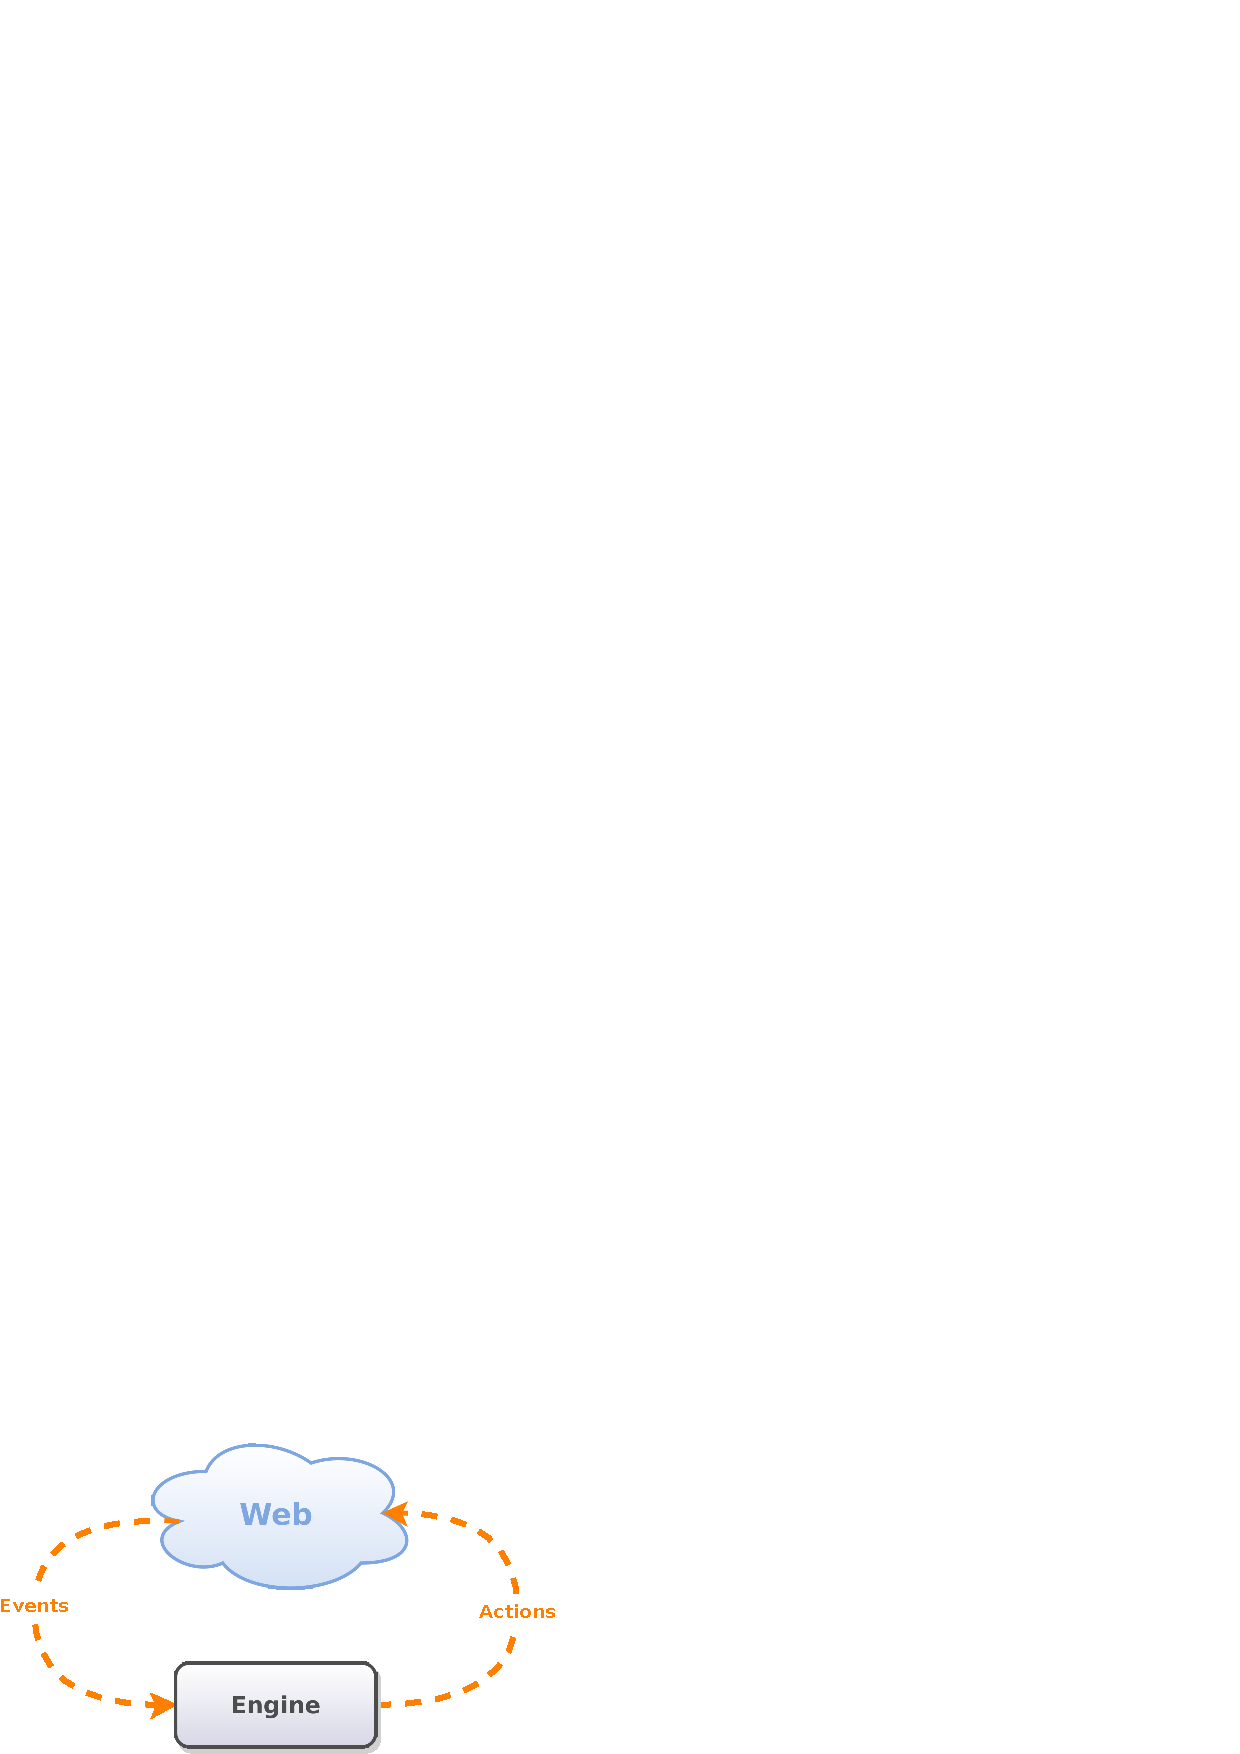
\includegraphics{figures/Conceptual_Model_Simple}
  \caption{SHOULD NOT SHOW UP}
  \label{fig:Conceptual_Model_Simpledummy}
\end{figure}

	
\chapter{Benchmarking}
\section{Java}
\section{JavaScript}


	
	\end{appendices}

	\addtocontents{toc}{\setcounter{tocdepth}{1}}

\backmatter
	
\pagestyle{empty}
\begin{figure}[p]
  \makebox[\linewidth]{
		\includegraphics[width=\paperwidth]{figures/scientificintegrity}
  }
\end{figure}

% 	\addtocontents{toc}{\setcounter{tocdepth}{1}}

\end{document}
